%%%%%%%%%%%%%%%%%%%%%%%%%%%%%%%%%%%%%%%%%%
%% TEX main file for the CLAS12 Nim Papers
%%       Do not edit this file
%%%%%%%%%%%%%%%%%%%%%%%%%%%%%%%%%%%%%%%%%%
\documentclass[3p,twocolumn]{elsarticle}
\renewcommand{\figurename}{Fig.}
%\usepackage{lineno, hyperref, multicol, color, xspace, pdfwidgets, enumerate, amssymb, textcomp, gensymb, verbatim, graphicx, subcaption}
\usepackage{lineno, hyperref, amssymb, subcaption}

\makeatletter
\def\ps@pprintTitle{%
 \let\@oddhead\@empty
 \let\@evenhead\@empty
 \def\@oddfoot{}%
 \let\@evenfoot\@oddfoot}
\makeatother

\modulolinenumbers[5]
\linenumbers

\journal{Nuclear Instruments and Methods A}

\begin{document}

\begin{frontmatter}
\title{The CLAS12 Forward Tagger} 

\author[CEAaddress]{A. Acker}
\author[CEAaddress]{D. Atti\'e}
\author[CEAaddress]{S. Aune}
\author[CEAaddress]{J. Ball}
\author[CEAaddress]{P. Baron}
\author[YORKaddress]{M. Bashkanov}
\author[GEaddress]{M.Battaglieri\corref{mycorrespondingauthor}}
\cortext[mycorrespondingauthor]{Corresponding author}
\ead{marco.battaglieri@ge.infn.it}
\author[DUQaddress]{R. Behary}
\author[DUQaddress]{F. Benmokhtar}
\author[GEaddress]{A. Bersani}
\author[CEAaddress]{Q. Bertrand}
\author[CEAaddress]{D. Besin}
\author[CEAaddress]{T. Bey}
\author[EDINaddress]{P. Black}
\author[JLABaddress]{P. Bonneau}
\author[CEAaddress]{R. Boudouin}
\author[CEAaddress]{M. Boyer}
\author[JLABaddress]{P. Campero Rojas}
\author[GEaddress]{A. Casale}
\author[GEaddress]{A. Celentano}
\author[GEaddress]{R. Cereseto}
\author[RM2address,UNIRTVaddress]{A. Ciarma}
\author[GEaddress]{F. Cipro}
\author[CEAaddress]{G. Charles}
\author[CEAaddress]{G. Christiaens}
\author[CEAaddress]{P. Contrepois}
\author[JLABaddress]{M. Cook}
\author[RM2address,UNIRTVaddress]{A. D'Angelo}
\author[GEaddress]{R. De Vita}
\author[CEAaddress]{M. Defurne}
\author[CEAaddress]{E. Delagnes}
\author[GEaddress]{E. Fanchini}
\author[GWUaddress]{S. Fegan}
\author[EDINaddress]{J. Flemming}
\author[TOaddress]{A. Filippi}
\author[CEAaddress]{M. Gar\c con}
\author[CEAaddress]{F. Georges}
\author[JMUaddress]{K.L. Giovanetti}
\author[GUaddress]{D.I. Glazier}
\author[CEAaddress]{R. Granelli}
\author[CEAaddress]{N. Grouas}
\author[OHIOaddress]{K. Hicks}
\author[JLABaddress]{A. Hoebel}
\author[EDINaddress]{S. Hughes}
\author[CEAaddress]{C. Lahonde}
\author[RM2address,UNIRTVaddress]{L. Lanza}
\author[JLABaddress]{M. Leffel}
\author[CEAaddress]{T. Lerch}
\author[GUaddress]{K. Livingston}
\author[CEAaddress]{I. Mandjavidze}
\author[JMUaddress]{H. S. Mann}
\author[GUaddress]{B. McKinnon}
\author[CEAaddress]{O. Meunier}
\author[JLABaddress]{R. Miller}
\author[GEaddress]{G. Min\'i}
\author[CEAaddress]{Y. Mouden}
\author[GEaddress]{P. Musico}
\author[GEaddress]{M. Osipenko}
\author[GEaddress]{G. Ottonello}
\author[GEaddress]{F. Parodi}
\author[JLABaddress]{E. Pasyuk}
\author[GEaddress]{P. Pollovio}
\author[GEaddress]{F. Pratolongo}
\author[CEAaddress]{S. Procureur}
\author[GEaddress]{R. Puppo}
\author[GEaddress]{C. Rossi}
\author[CEAaddress]{M. Riallot}
\author[GEaddress]{M. Ripani}
\author[RM2address,UNIRTVaddress]{A. Rizzo}
\author[CEAaddress]{F. Sabati\'e}
\author[NSUaddress]{C. Salgado}
\author[EDINaddress]{G. Smith}
\author[GUaddress]{D. Sokhan}
\author[EDINaddress]{I. Stankovic}
\author[GEaddress,UNIGEaddress]{M. Taiuti}
\author[GEaddress]{A. Trovato}
\author[CEAaddress]{M. Vandenbroucke}
\author[CEAaddress]{E. Virique}
\author[YORKaddress]{D. Watts}
\author[JLABaddress]{C. Wiggins}
\author[YORKaddress]{N. Zachariou}
\author[JLABaddress]{L. Zana}

\address[CEAaddress]{IRFU, CEA, Universit\'e Paris-Saclay, F-91191 Gif-sur-Yvette, France}
\address[YORKaddress]{University of York, York YO10 5DD, United Kingdom}
\address[GEaddress]{INFN - Sezione di Genova, Via Dodecaneso 33, I-16146 Genova,Italy}
\address[DUQaddress]{Duquesne University, Pittsburgh, PA 15282, USA}
\address[RM2address]{INFN, Sezione di Roma Tor Vergata, 00133 Rome, Italy}
\address[UNIRTVaddress]{Universit\'a di Roma Tor Vergata, 00133 Rome Italy} 
\address[GWUaddress]{The George Washington University, Washington, DC 20052, USA}
\address[EDINaddress]{University of Edinburgh, Edinburgh EH9 3FD, United Kingdom}
\address[TOaddress]{INFN, Sezione di Torino, 10125 Torino, Italy}
\address[JMUaddress]{James Madison University, Harrisonburg, VA 22807, USA}
\address[GUaddress]{University of Glasgow, Glasgow G12 8QQ, United Kingdom}
\address[OHIOaddress]{Ohio University, Athens, OH 45701, USA}
\address[NSUaddress]{Norfolk State University, Norfolk, VA 23504, USA}
\address[UNIGEaddress]{Universit\'a degli Studi di Genova, Via Dodecaneso 33, I-16146 Genova,Italy} 
\address[JLABaddress]{Thomas Jefferson National Accelerator Facility, Newport News, VA 23606, USA}

\begin{abstract}The High Threshold Cerenkov Counter (HTCC) is one of the detector systems of the CLAS12 spectrometer, and is used to generate fast trigger signal in electron experiments. The HTCC is installed in front of the R1 Drift Chambers and introduces a minimal amount of additional material within working acceptance. The HTCC is one unit whose core component is a multifocal mirror that consists of 60 lightweight composite ellipsoidal mirrors. It is important that the HTCC provides efficient coverage of the CLAS12 acceptance with no gaps or overlaps. In order to achieve this, each sector of the CLAS12 spectrometer is covered by 2 identical half-sector mirrors that focuses Cerenkov light on eight phototubes. The HTCC has a total of 48 channels with Electron Tubes 9823QKB PMTs that have a 5" quartz face plate to detect Cerenkov light. The system provides a high rejection of charged $\pi$-mesons and low background noise for reliable identification of scattered electrons. The details of the design, construction, calibration, and performance results of the HTCC are presented in the following paper. 

\end{abstract}

\end{frontmatter}

\date{\today}

\section{Overview}

torus overview description \cite{einstein}



\section{Requirements}

torus requirements description


% \section{Design(Chris, Sergey)}

CLAS12 Data Aquisition system is designed as pipeline-style network-based system. Data taking process starts from front-end components. Those components can have different hardware and software implementation but have to follow certain requirements to be compatible with the rest of the system. Currently front-end components used are commercial VME/VXS crates, commercial Linux servers and JLAB-designed VXS Trigger processor boards. VTPs installed in VXS crates but read out by DAQ as independent components. All components are running on 250MHz clock discributed over OM3 rated parallel optic fibers. The same fiber system is used to distribute sync reset and trigger signals and to collect busy signals from all front-end electronics.

All front-end components are connected to Event Builder (EB) which is multi-threaded program running on multi-core Linux server. Most connections are 1Gbit ethernet links. For several components generating significant data rate 10Gbit ethernet connection is used.

Complete events are sent to Event Transfer (ET) System. ET is multi-threaded program providing data ring where various data processing programs can be attached to monitor data quality online. It can be run on the same server as EB, or can be used to create sequensial chain of servers to increase data processing power.

Last component in the data chain is Event Recorder (ER). It is multi-threaded program receiving data from ET system and recording it to the disk. Multi-stream mode is available, allowing to write several files in parallel to the same or different disk partitions to increase writing performance. Event order in multi-stream mode is preserved.

CLAS12 DAQ System diagram is shown on Fig.~\ref{fig:DAQdiagram}.

\begin{figure}[hbt]
	\centering
	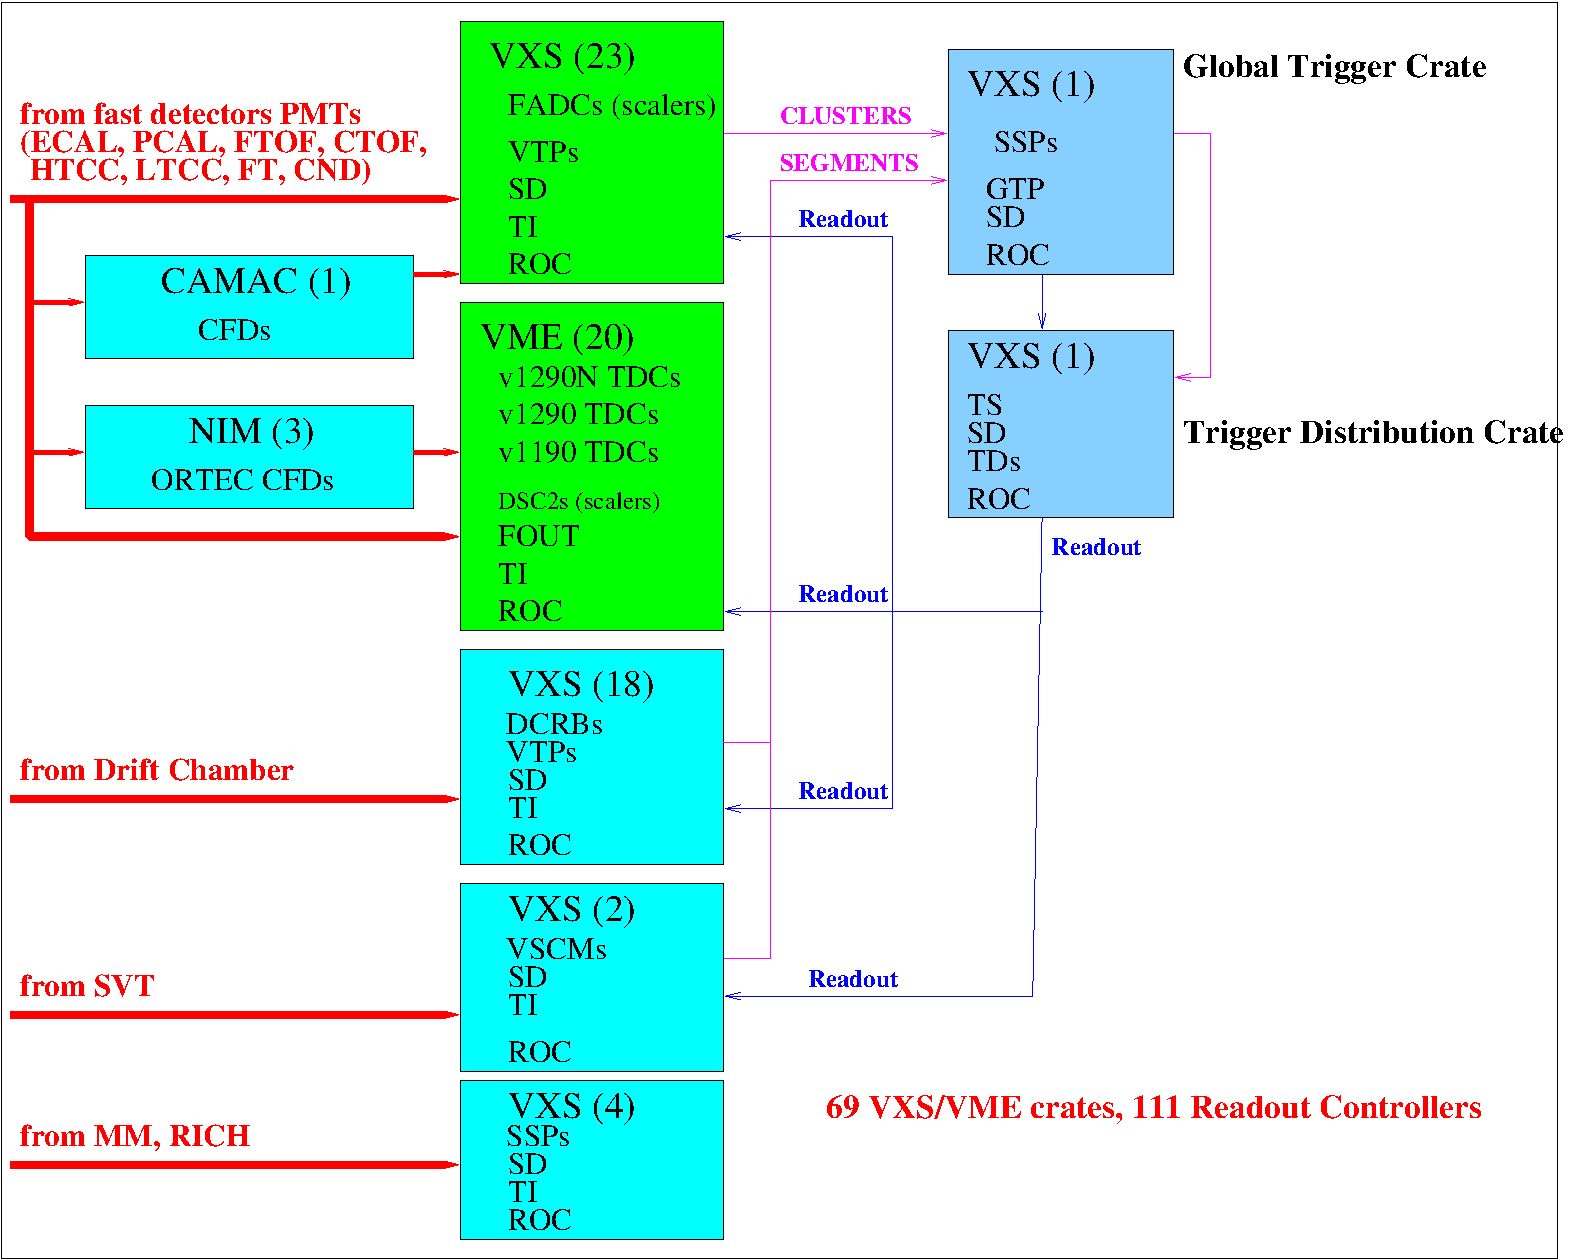
\includegraphics[width=1.0\columnwidth,keepaspectratio]{img/CLAS12_HARDWARE_2.pdf}
	\caption{CLAS12 Data Aquisition System Diagram}
	\label{fig:DAQdiagram}
\end{figure}


\section{Hardware Components}

New instrumentation modules have been designed by JLab that take advantage of the higher performance and elegant back-plane connectivity of the VITA 41 standard or ``VXS'', defined as VME with serial extensions. 
VXS was selected as the 12~GeV data acquisition back-plane foundation for the front-end detector readout and trigger hardware interface because this standard offered a method to easily synchronize and pass signals between each of the payload slots to a central switch fabric slot. At JLab a dual star back-plane configuration is used, and one switch slot is used for the trigger processing and one switch slot is used to distribute the essential timing and synchronization signals to each of the front-end boards.

The trigger processor switch slot board manages the high-speed gigabit signaling from each of the payload slots, where eight differential pairs connect from the payload slots to the switch slots. The VXS crates are manufactured by WIENER and the back-plane can support up to 8~Gb/s. The payload boards use Xilinx Virtex V technology, and these FPGAs have up to 6.25~Gbps transceivers. The payload boards are designed to run these high-speed gigabit transceivers at a maximum of 5~Gpbs to transfer trigger data to the trigger processor module. 

The design challenges for reliable and successful transmission of gigabit serial data over the VXS backplane requires the investment of high-speed circuit board layout and routing tools.  The FPGA selection requirements include at least four full duplex gigabit transceivers, user I/O pin count $>$~500, and fast integrated block memory with multi-rate FIFO logic. We use circuit board routing simulation tools such as Mentor Graphics HyperLynx [\ref], which are invaluable for critical simulation and verification of circuit board signal integrity for the gigabit transmission paths before the manufacturing process.  The FPGA devices that we use are capable of 6.25~Gb/s serial transfer, and we have designed our circuit boards with signal integrity techniques using standard FR4 circuit board material to achieve $>$~2.5~Gb/s, which meets the data transfer bandwidth requirements. 
Another significant investment required for the hardware verification of the gigabit transceivers was a digital signal analyzer with 8~GHz bandwidth to measure and record the backplane and fiber optic gigabit transceiver performance and to perform jitter analysis on the critical system clock and synchronization signals with at least 1~ps resolution.  We used the Tektronix jitter analysis software which is a critical tool for the verification of our system clock, and for measurements of the phase controlled jitter attenuated clock provided by the Signal Distribution (SD) switch card in every crate. The investment of firmware development tools from FPGA industry leaders Xilinx and Altera were also taken into consideration for the upgrade path to VXS. We use the Xilinx Aurora protocol for serial transmission as it is robust and simple, and is included with the FPGA development tools.  


\subsection{Fiber Optic Trigger distribution system}

As shown in Fig.~\ref{fig:hardwarediagram}, the digital sum value from each VTP in the front-end crate, and the distribution of the global clock, synchronization, and trigger commands from the global trigger hardware, use a separate fiber optic cable.  The crate sum fiber link is shown in orange, and the critical timing signals distributed to each front-end crate are blue.  Each fiber optic link makes use of the Avago POP4 fiber optic transceivers and parallel OM3-rated glass fiber cable with MTP connections. These fiber optic transceivers operate at 3.125~Gb/s for an aggregate bandwidth of 10 Gb/s which is ample enough for the summing information that is sent forward to the global trigger processing hardware.  The fiber link used for the distribution of the global clock, critical timing signals, and trigger commands runs at 1.25~Gb/s.

\begin{figure}[hbt]
	\centering
	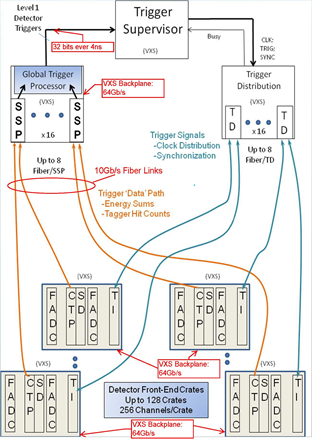
\includegraphics[width=1.0\columnwidth,keepaspectratio]{img/hardware_diagram.png}
	\caption{Hardware diagram with the implemented fiber links scheme.}
	\label{fig:hardwarediagram}
\end{figure}


\subsection{VXS/VME crates}

Previous experiments with the original CLAS spectrometer (see \cite{clas-nim}) used the VXI standard, which was a new extension of the original VME standard. VXI offered a method to distribute clock and other timing signals with low skews via the back-plane. 9U circuit boards were used that offered a large number of front panel input/output connections to handle the six sectors of the CLAS detectors that contributed to the level 1 trigger. The detector signals were acquired with FastBus ADC and TDC or in some instances, from VME or even CAMAC modules. 

During the initial design phase of the 12~GeV experiments the requirements of a 200~KHz sustained trigger rate demanded that the front-end modules adopt a new method of handling precision timing and synchronization over dozens of front-end crates. The latest technology at the 12~GeV inception included FPGA devices with high-speed serial transceivers built into the silicon fabric. A new VME extension was also emerging at the same time, which was labeled VXS, and defined a new high-speed gigabit connector with links between the VME slots and eight serial links to common switch slots. The VXS standard was declared as VITA 41 and several new standards have emerged in the past decade that expand the use of gigabit serial transmission via the crate back-plane. For the 12~GeV experiment era, we now have thousands of custom VXS payload and switch slot modules and hundreds of VXS front-end crates. Complex experiments and high channel count detectors make use of these custom VXS boards  designs for all four experimental halls at JLab.

\subsection{VME Crate Controllers}

The high-speed data physics acquistion and trigger systems for the JLab 12~GeV experiments have been standardized on the VME64X and VXS backplane and crate enclosure form-factor. In addition to the custom electronics that reside in these crates, there must also be a single ``controller'' for each crate. Considering all four experimental halls, this exceeds 100 controllers.

There are many commercial off-the-shelf options for this type of controller, and our general requirements do not extend beyond what is currently commercially available. We do have some specific requirements that narrowed the viable choices.

We purchased VME controllers from several vendors for development purposes and made a significant investment in custom software that runs on all of the existing boards. We also benchmarked our code and have come to expect certain ``minimum'' requirements for performance from the chosen architecture within an specified Linux operating system.

We also expect a certain minimum 10 year timeframe in which these controllers will be supported by the vendor with respect to the avilable parts, repair, and software updates. VME controller requirements are summerized in following list:

\begin{itemize}
	\item Single slot VME form-factor - no required rear transition module
	\item Intel Core i7 dual or quad core embedded processer 2~GHz (or greater)
	\item Hyperthreading and 64~bit arch support
	\item 4 GBytes DDR3 (1066~MHz) ECC SDRAM (or greater)
	\item Front panel gigabit ethernet and serial port console
	\item 1 x4 PCI Express XMC expansion slot (or greater)
	\item VME320-interface using the Tundra Tsi148 chip
	\item support for all VME transfer modes including 2eSST
	\item VXS optional: interface supporting both VITA 41.3 (Gig E) and 41.4 (PCIe) standards.
\end{itemize}

After several different boards were evaluated we purchased XVR16 Intel forth Generation 4-core i7-based rugged VME single board computers from GE (see Fig.~\ref{fig:XVR16diagram}). They were installed in the 70+ crates for CLAS12 and have demonstrated excellent performance and reliability. Most of the controllers send data over their built-in 1~GBit link, while for few of them, a 10~GBit daughter board was installed to increase the bandwidth. The maximum data rate from a single crate in CLAS12 never exceeds 130~MB/s, and with that rate 4-core controllers are able to handle the VME data polling, data processing, and sending data over the network without any issues. 

\begin{figure}[hbt]
	\centering
	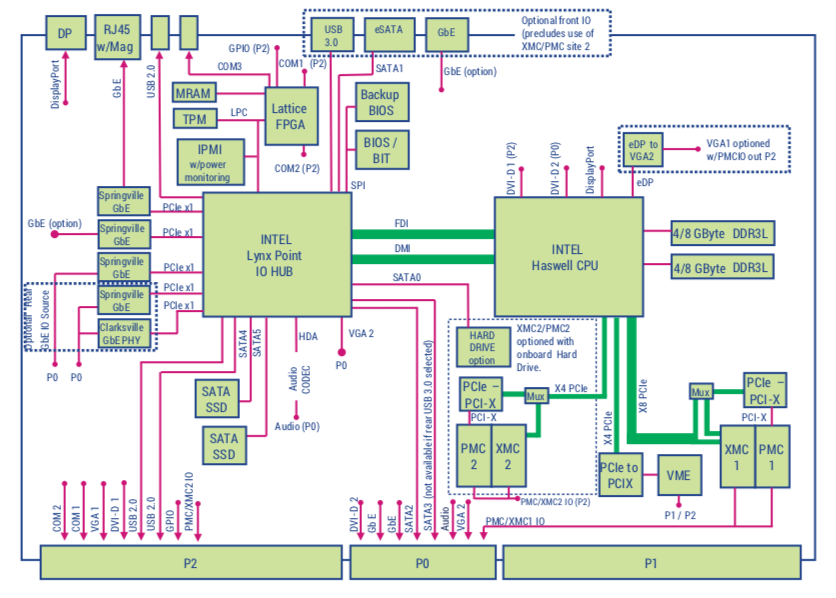
\includegraphics[width=1.0\columnwidth,keepaspectratio]{img/XVR16_diagram.png}
	\caption{Block diagram of the XVR16 VME crate controller}
	\label{fig:XVR16diagram}
\end{figure}



\subsection{Trigger Distribution System Modules (TS, TD, TI)}
	
The TCS (TRIGGER, CLOCK, SYNC, and BUSY) distribution system \cite{tcs-ref} is the hardware interface to bridge the trigger and the DAQ.  The TCS system receives the trigger decision from the trigger system, and initiates data readout for the DAQ system by distributing the readout trigger (TRIGGER) signal.  Additionally, it distributes a 250~MHz system clock (CLOCK) to pipeline the system, and it distributes an encoded synchronous signal (SYNC) for the system synchronization.  It monitors the frontend electronics’ status (BUSY) and makes sure of the smooth data readout of the experiments. Fig.~\ref{fig:TCSdiagram} shows a diagram of the trigger and TCS distribution.

\begin{figure}[hbt]
	\centering
	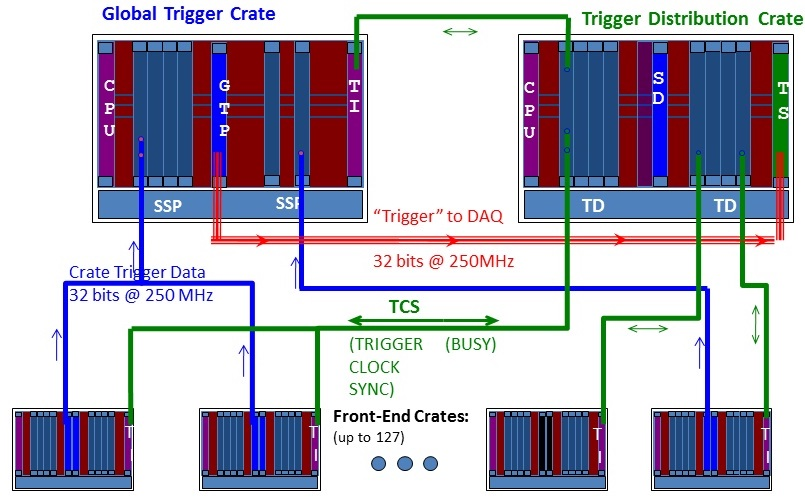
\includegraphics[width=1.0\columnwidth,keepaspectratio]{img/TCSdiagram.jpg}
	\caption{Diagram of the trigger and TCS distribution. The VTP boards generate triggers using detector signals from the front end crates.  The final trigger decisions, up to 32 trigger types, are sent from VTP to TS for data readout.  The TS distributes the TCS to the TD through SD and the backplane, then to the front end crate through optic fiber and TI.  The TI collects the front end boards busy signals and sends to TD, then throttle (disable) the readout trigger distribution on TS.
}
	\label{fig:TCSdiagram}
\end{figure}


The main hardware of the TCS distribution system includes a Trigger Supervisor (TS \cite{ts-ref}) board (see Fig.~\ref{fig:TSused} and ~\ref{fig:TSdiagram}), Signal Distribution (SD \cite{sd-ref}) boards, Trigger Distribution (TD \cite{td-ref}) boards  (see Fig.~\ref{fig:TDused}), Trigger Interface (TI \cite{ti-ref}) boards  (see Fig.~\ref{fig:TIused} and ~\ref{fig:TIdiagram}), VXS crates, and optic fibers.  The TS board, one SD board, and up to sixteen TD boards are located in the global TCS distribution VXS crate.  One TI board and one SD board and/or one FANIO board are located in each front-end crate.  The electronics boards were custom designed and produced for the 12 GeV upgrade.  Field Programmable Gate Arrays (FPGA) are used for TCS generation, control, and decoding.  Optical fibers and high-speed differential backplane connections are used to transmit signals at high speed over long distances.  

\begin{figure}[hbt]
	\centering
	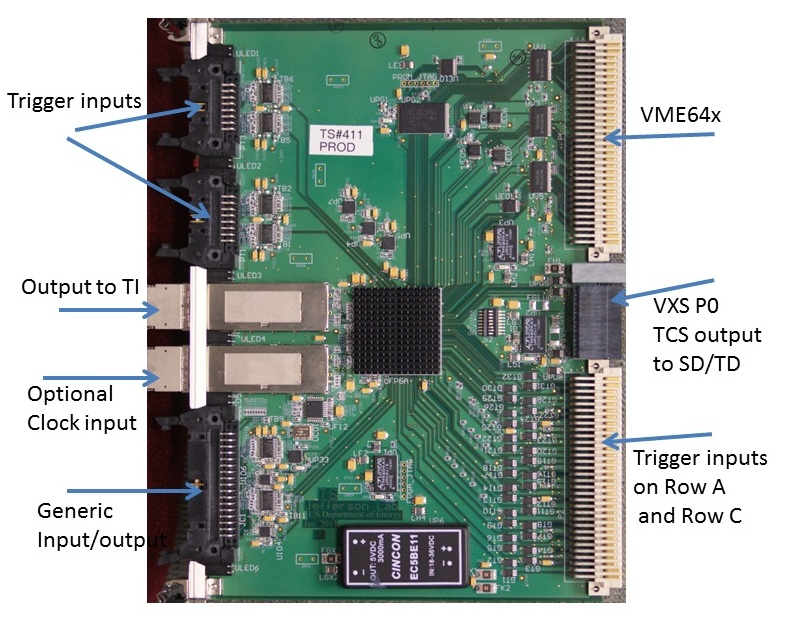
\includegraphics[width=1.0\columnwidth,keepaspectratio]{img/TSused.jpg}
	\caption{Trigger Supervisor (TS) board.  The TS board is a 6U by 160mm VME board with VXS connector.  It generates and distributes the readout triggers, synchronization signals, and clock (either from the front panel input or the on-board oscillator) to the TD boards via the SD through the VXS backplane.}
	\label{fig:TSused}
\end{figure}

\begin{figure}[hbt]
	\centering
	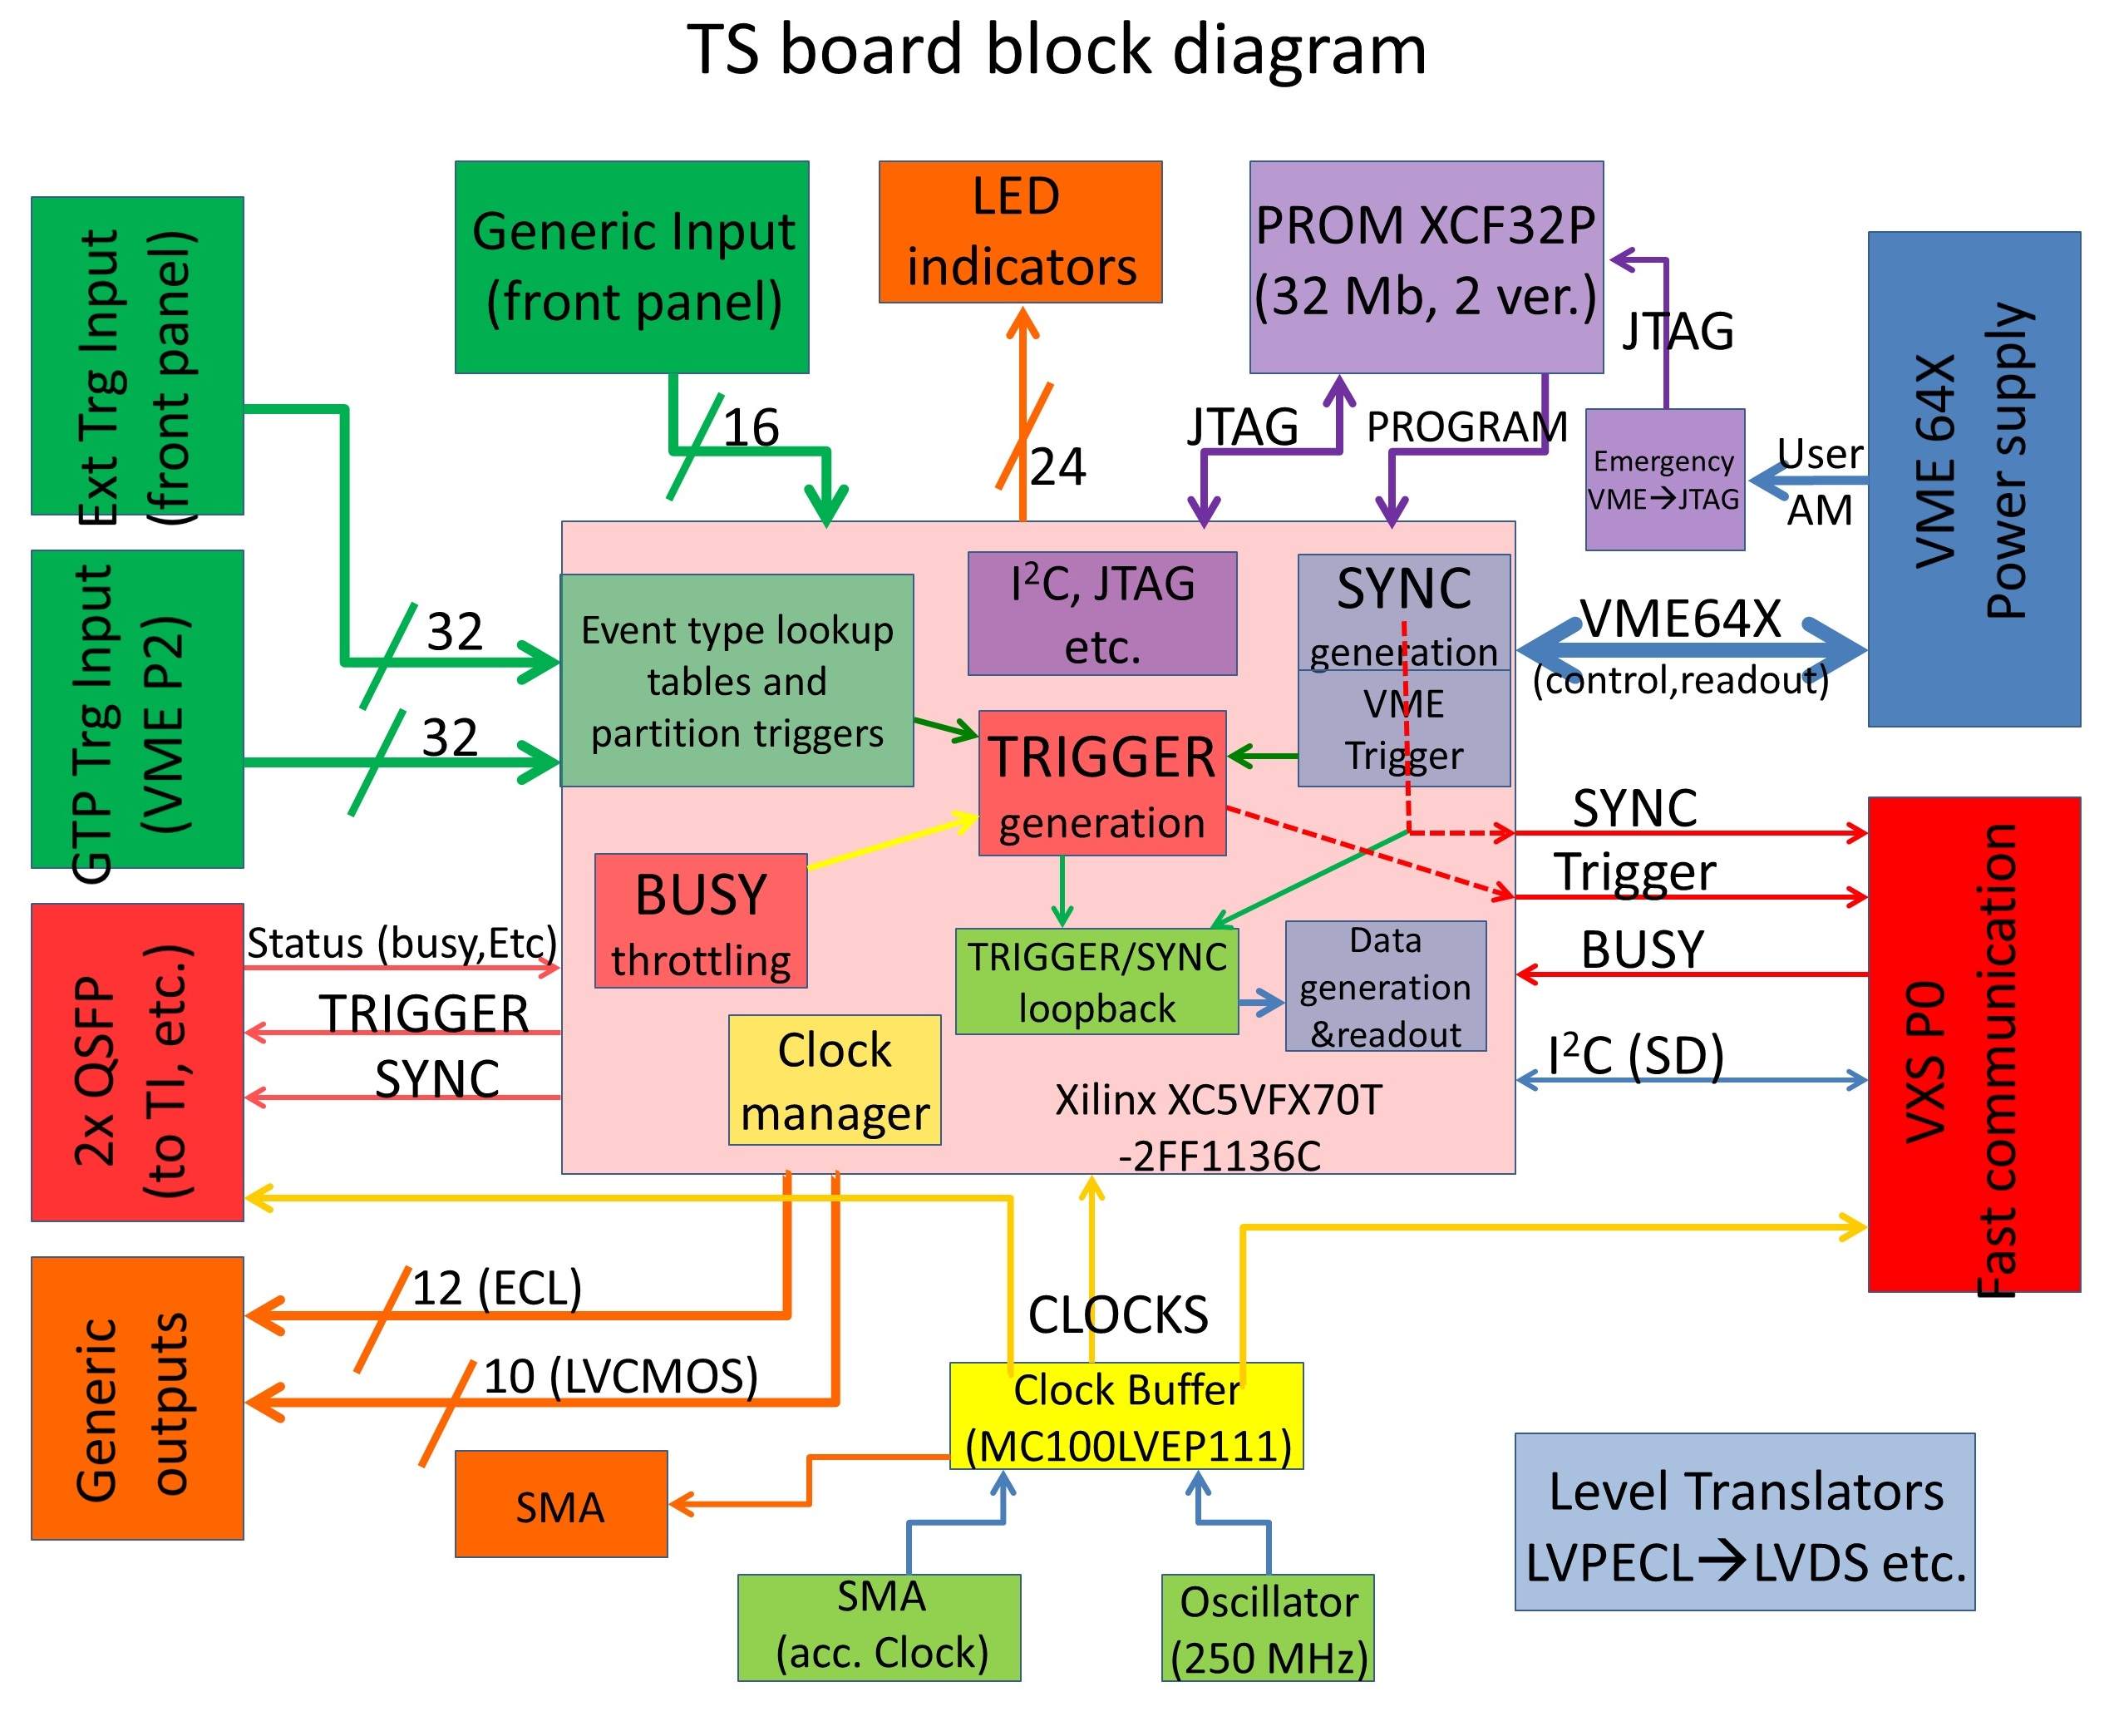
\includegraphics[width=1.0\columnwidth,keepaspectratio]{img/TSdiagram.jpg}
	\caption{TS board diagram.  The TS generates the readout triggers from up to 32 front panel trigger inputs and up to 32 backplane trigger inputs (from GTP), and sends out the triggers via encoded 16-bit words to the backplane.}
	\label{fig:TSdiagram}
\end{figure}

\begin{figure}[hbt]
	\centering
	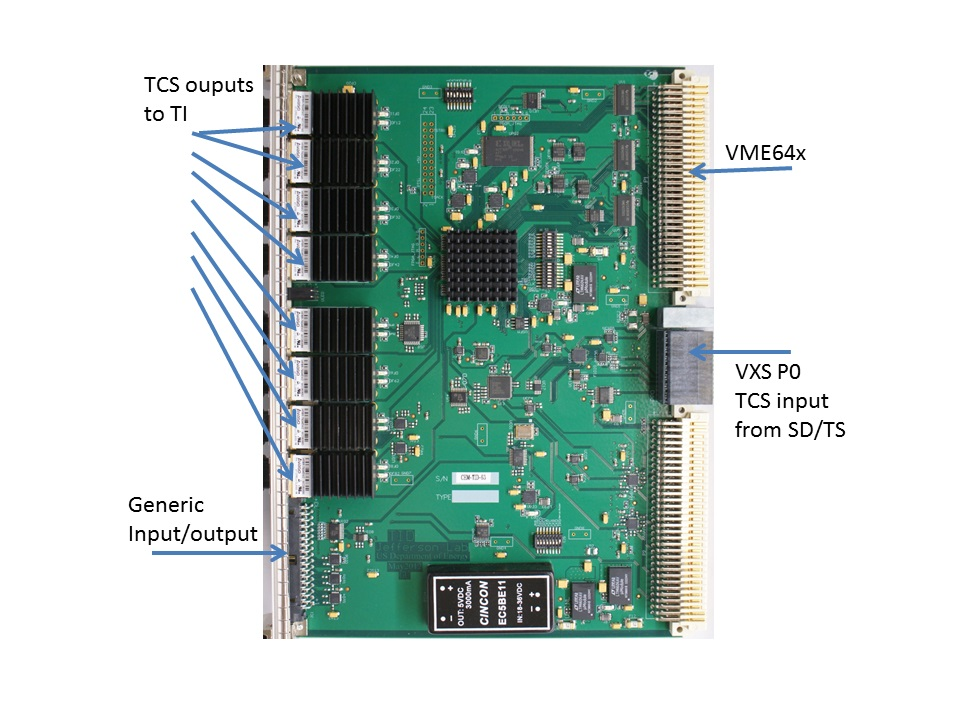
\includegraphics[width=1.0\columnwidth,keepaspectratio]{img/TDused.jpg}
	\caption{Trigger Distribution (TD) board.  The TD board is a 6U by 160mm VME board with VXS connector.  It receives the TCS from TS via the VXS backplane, and distributes the TCS via the front panel QSFP optic links.  It collects the Busy inputs from up to eight TI boards, and generates the readout buffer busies for up to eight front end crates.  The TD sends the collective BUSY to TS to back pressure the trigger generation.}
	\label{fig:TDused}
\end{figure}

\begin{figure}[hbt]
	\centering
	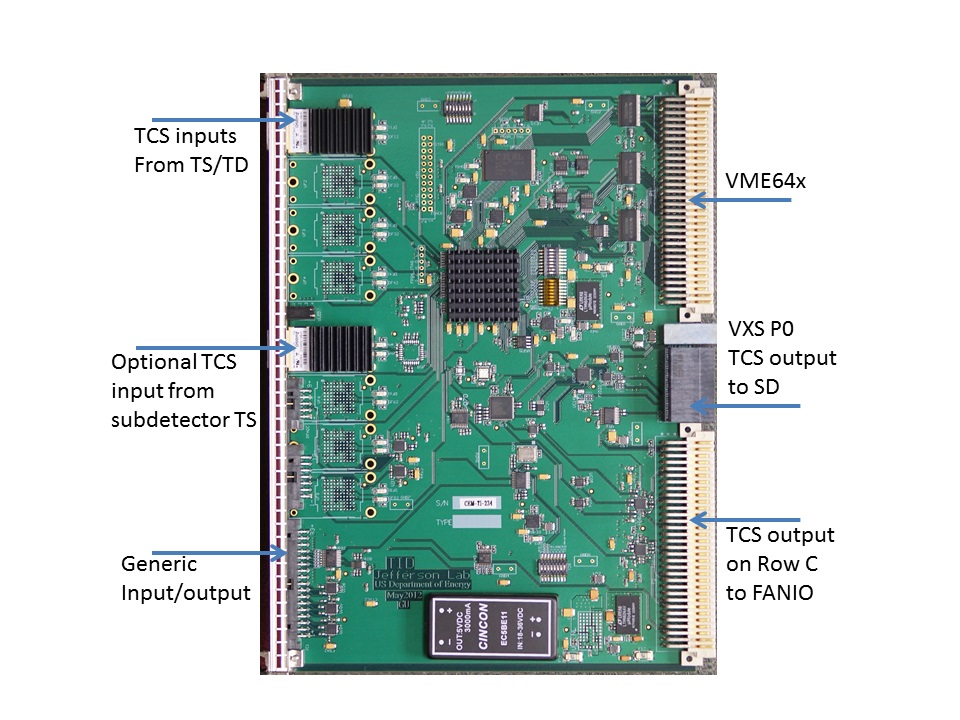
\includegraphics[width=1.0\columnwidth,keepaspectratio]{img/TIused.jpg}
	\caption{Trigger Interface (TI) board.  The TI board is a 6U by 160 mm VME board with (or without) the VXS connector.  It is using the same PCB as TD board with modified components population.  It receives the TCS from TS/TD or a sub-system controller via fiber, and collects the busy and sends to TS/TD via the same fiber.  The TI can also be used as a subsystem controller in the so-called master mode.}
	\label{fig:TIused}
\end{figure}

\begin{figure}[hbt]
	\centering
	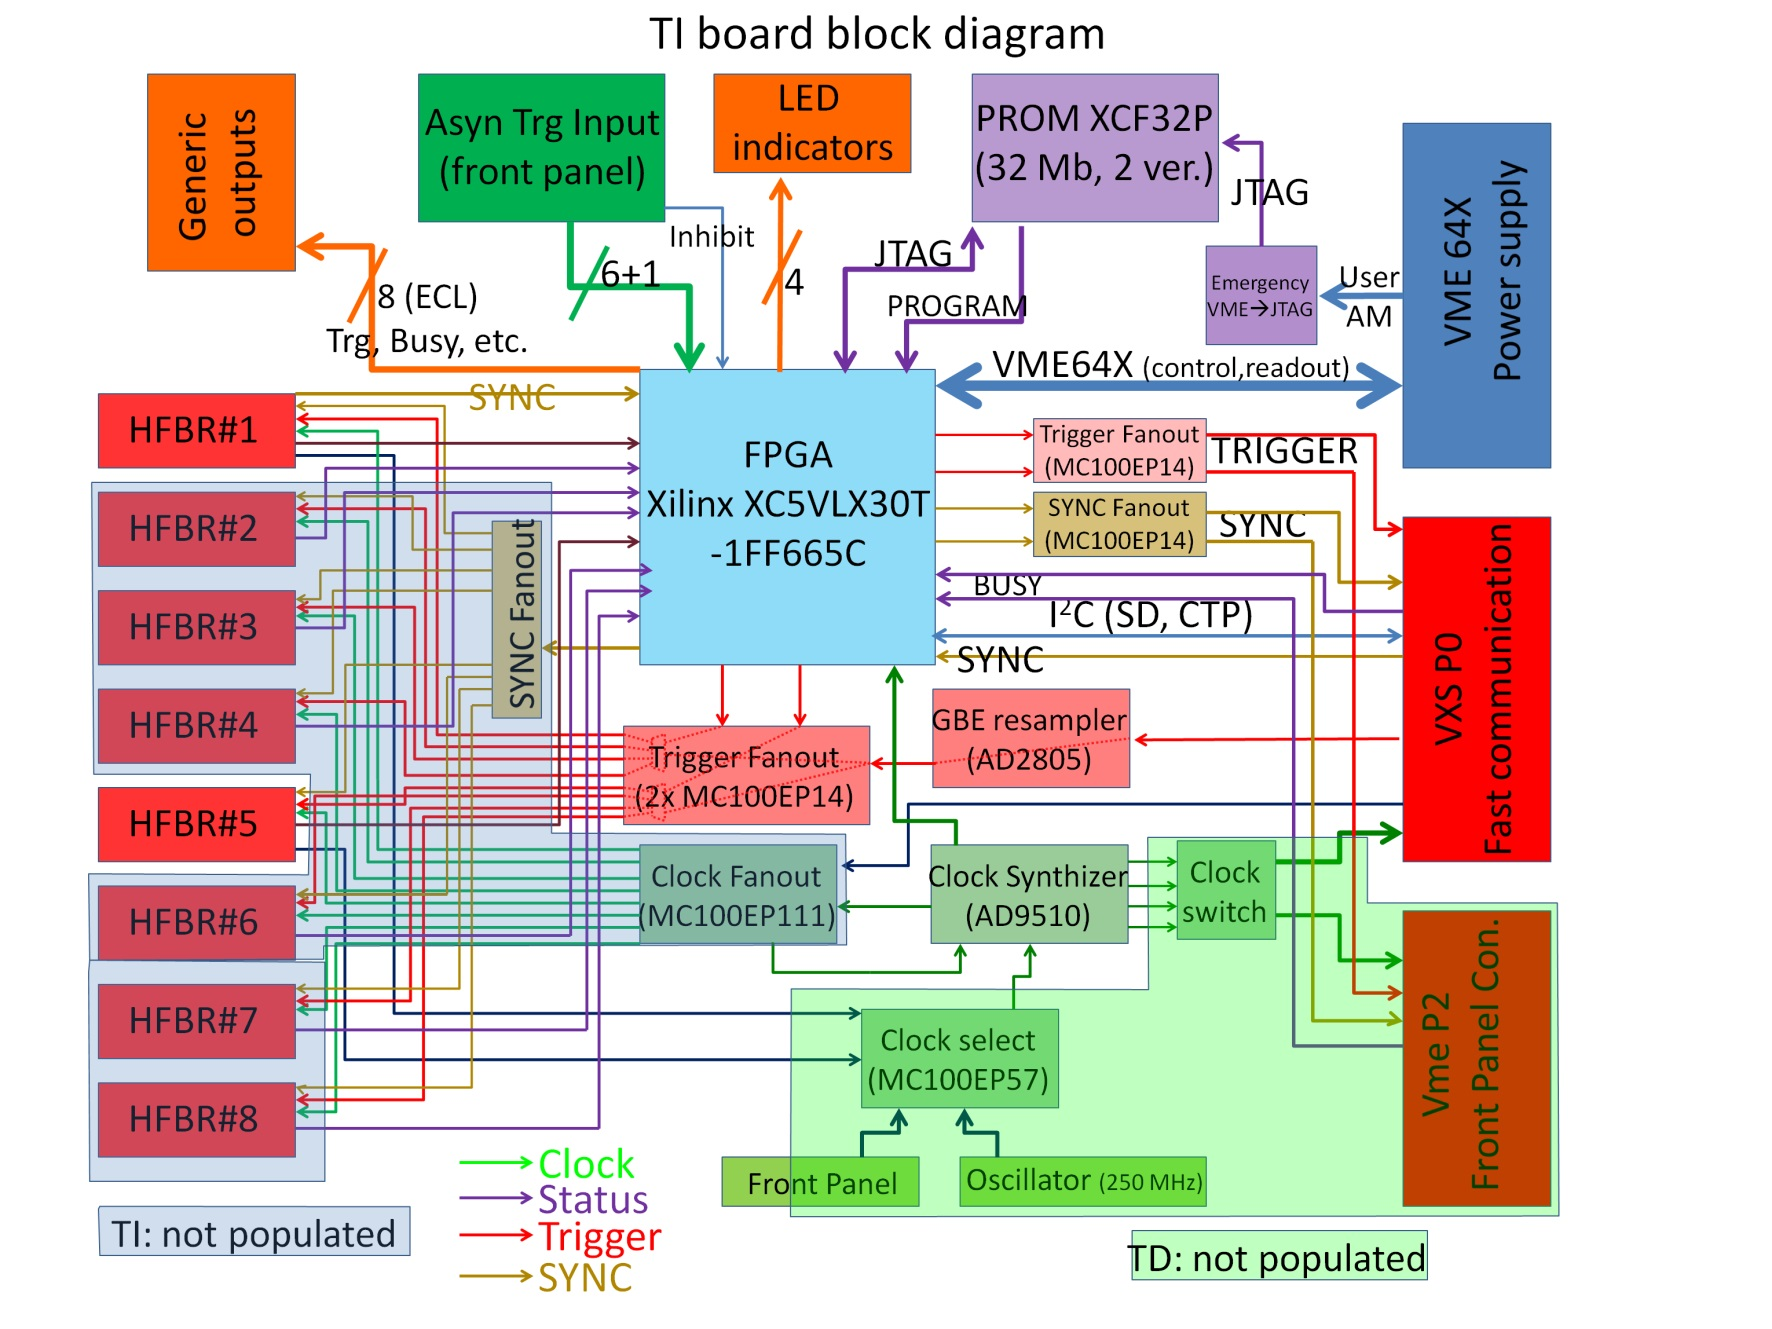
\includegraphics[width=1.0\columnwidth,keepaspectratio]{img/TIdiagram.jpg}
	\caption{TI and TD board diagram.  The TI and TD use the same PCB design, but different component population and FPGA firmware.}
	\label{fig:TIdiagram}
\end{figure}


\subsubsection{Clock Distribution}

The TCS system uses the 250 MHz clock, that comes from the TS in the global trigger distribution crate.  This clock is either generated by the TS on-board oscillator or its fronts panel input.  The clock is fanned out to the VXS P0 connector and then to the SD board.  The SD fans out the clock to the TD boards via the VXS P0 backplane.  The TD boards further fan out to the TI boards via optic fibers.  The TI uses this clock to generate clocks with proper frequencies (250 MHz, 125 MHz, 62.5 MHz, 31.25 MHz and 41.67 MHz) and sends the clocks to the front-end crate SD board, and the SD fans out to the front-end DAQ modules (TDC, ADC).  The fan-out buffer level is minimized on every board to limit the clock jitter.  The slower clocks derived from the main system clock are phase aligned thanks to the Analog Devices AD9510 with a synchronous phase re-alignment command.  The clock jitter is about one ps measured at the front-end electronics.  The clock distribution skew can be adjusted by the SD clock delay if necessary.


\subsubsection{SYNC Distribution}

The TS generates and distributes the SYNC signal.  The SYNC is an encoded 4-bit serialized command transferred at 250 Mbps synchronized with the system clock.  Normally, the serial SYNC line stays at logic high (or ‘1’).  When transferring a SYNC command, the SYNC goes to logic low for one bit, followed by the 4-bit command code.  After the 4-bit SYNC command, the SYNC goes to logic high again.  There is a minimum of four ‘1’s before the next cycle begins.  The SYNC start is phase aligned to the 62.5 MHz clock used for the trigger word transfer, the 41.67 MHz clock used for the CAEN TDC boards, and the 31.25 MHz clock used for Flash ADC boards.  This phase relation is used to synchronize the slower clocks on the TI to the 62.5 MHz clock on the TS.  This also limits the SYNC command to no more than one per 96 ns.  To facilitate the AC coupled optical transceivers, the SYNC is Manchester encoded on the TS and the TD, and Manchester decoded on the TI and the TD.

The SYNC is phase aligned with the 250 MHz system clock on the TI boards using their FPGA’s IODELAY.  The SYNC is synchronized across the TI boards by applying different delays on the individual TI boards.  The delays are determined by the fiber latency measurement.  

The spare fibers between the TD and TI boards are used to measure the fiber latency.  The TI sends a test signal to the TD through one fiber, and the TD loops back the signal through another fiber.  The TI measures the delay between the test pulse and the looped back test pulse using the FPGA counter and the carry chain in the FPGA.  As the fiber skew is small (less than 1 ns for 100 meter fibres), the measurement on these two fibres can be used as the latency of the other fibres in the cable.  
After the SYNC latency compensation, all the TI boards receive the SYNC at the same time with the skew of one system clock period, which is 4 ns.  The synchronized SYNC signals are used to synchronize the triggers as described next.


\subsubsection{Trigger Distribution}

The trigger words, which include the readout trigger signals and event information (event type, trigger timing, etc.), are generated and serialized on the TS.  The serialized trigger word is fanned out by the SD board and the TD board, and deserialized by the TI board.  The 16-bit trigger words are summarized in Table~\ref{tab:trigger_word_definition}.  

\begin{table}
\begin{adjustbox}{width=\columnwidth,center}
	\begin{tabular}{| l | l | l | l |}
		\hline \hline
		Bit 15:12		& 	Bit 11:10 &	Bit 9-0	 & Comment		\\
		\hline
	1001	& Quadrant timing	& Event type	 & GTP major trigger \\
	1010	& Quadrant timing	& Event type	 & Ext major trigger \\
	
	1011	& \multicolumn{2}{c}{Four TS partitions’ event types}    & TS partitioning (4, 3, 2, 1) \\

	\multirow{2}{*}{0110}	& \multirow{2}{*}{Quadrant timing}	& Trigger source & TImaster legacy Trigger \\
		    &                   & Event type	 & (TS) VME trigger     \\
	0101	& Trigger command/Control	& VME command \\
	0100	& TS timer (TS time bit(13:2))	& TI Sync check \\
	0111	& Trigger content	& Additional trigger info \\
		\hline \hline
	\end{tabular}
\end{adjustbox}
\caption{Trigger word definition.  The TS encode the readout trigger, event type, and the fine timing (4ns quadrant) information into a 16-bit word, which is transferred every 16ns.  This 16-bit word can also be some system setting information or the system timer when there is no readout trigger in the 16ns periods.}
\label{tab:trigger_word_definition.}
\end{table}

Both the fiber latency and trigger word serializer/ deserializer are compensated so that all the TI boards send the readout trigger at the same time to the front-end data acquisition electronics.  The SYNC is used in conjunction with a synchronous FIFO to enforce a fixed latency on the trigger distribution. Fig.~\ref{fig:TIsync} shows the diagram of the compensated trigger distribution.

\begin{figure}[hbt]
	\centering
	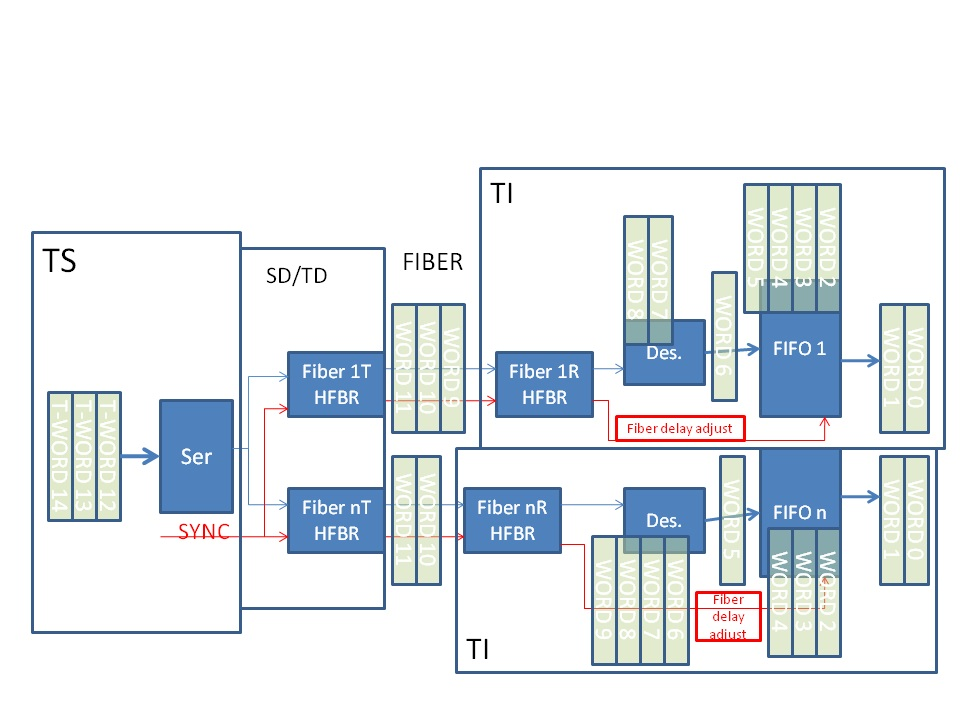
\includegraphics[width=1.0\columnwidth,keepaspectratio]{img/TrgSync.jpg}
	\caption{Trigger synchronization between TIs.  The TI boards delay the decoding of the received readout trigger by the complement of the TS/TD to TI transfer latency, so that all the front end boards receive the readout trigger simultaneously.}
	\label{fig:TIsync}
\end{figure}

On the TI board, the deserialized trigger word is clocked into and clocked out of a FIFO using the 62.5~MHz clock.  At the start-up, the FIFO is reset (0 words) and the FIFO read/write is disabled.  The serial trigger link is idle words only.  On trigger start, the TS starts trigger word transmission.  The TI will write the deserialized data (valid data, that is non-idle data word) to the FIFO.  After some pre-set delay (VME register controlled), the TS issues a ‘Trigger Start’ command on the SYNC link.  When TI receives the ‘Trigger Start’, the TI resets the trigger FIFO readout address, and enables continuous readout of the FIFO.  As the SYNC lines are fiber length adjusted and the 62.5 MHz clocks are phase aligned, the trigger words from the TI board FIFO are synchronized across the system.
The trigger word also has the fine trigger timing information.  By decoding that, the TI board distributes the trigger in 4 ns precision, although the trigger word is serialized every 16 ns.  If the system clock phase is not adjusted, there will be a maximum of 4 ns skew among the clocks on the TI boards, so does the readout trigger.  The clock phase can be adjusted by SD if the skew is critical to the system.


\subsubsection{DAQ synchronization (trigger throttling) control}

Because of the finite memory size and the randomness of the triggers, it is possible for the memory to become overwhelmed somewhere in the system, which could cause DAQ problems.   The TCS throttling mechanism is used to prevent possible memory overflows, and to keep the DAQ synchronized.  Fig.~\ref{fig:DAQ_synchronization} shows the DAQ synchronization logic implementation.  Three methods are used to keep the DAQ synchronized.  These include trigger rules and event limit setting, pipeline DAQ, and synchronization events (special events).

\begin{figure}[hbt]
	\centering
	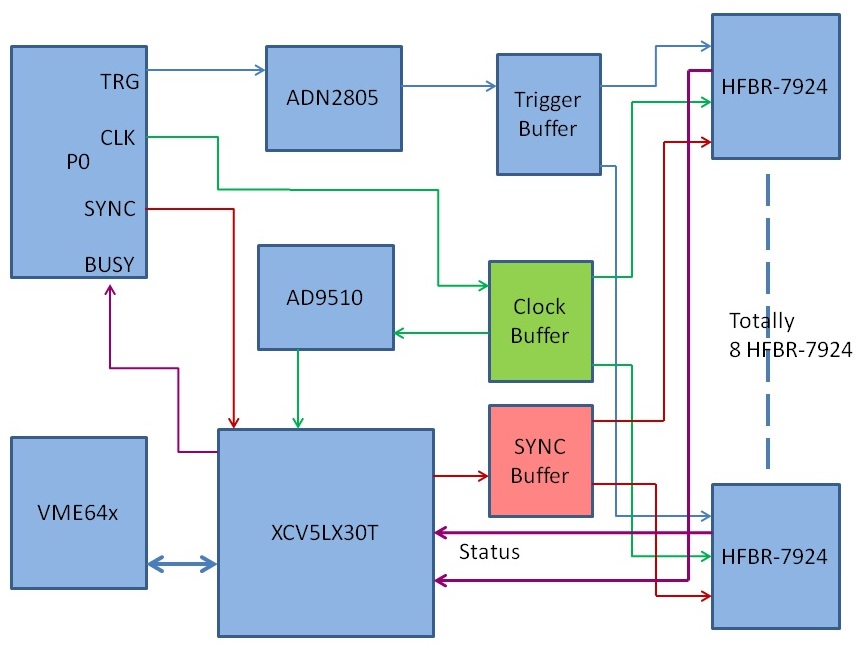
\includegraphics[width=1.0\columnwidth,keepaspectratio]{img/TDdiagram.jpg}
	\caption{DAQ synchronization}
	\label{fig:DAQ_synchronization}
\end{figure}


%REFERENCES
%[1] 	J. Gu etal. (2014, May). The TRIGGER/CLOCK/SYNC Distribution for TJNAF 12 GeV Upgrade Experiments    %https://coda.jlab.org/wiki/index.php/Trigger_distribution_overview
% [2] 	J. Gu. Description and technical information for the Trigger Supervisor (TS) module.  TJNAF, VA, 2013.  %Available: https://coda.jlab.org/drupal/system/files/pdfs/HardwareManual/TS/TS.pdf 
%[3] J. Gu, etal, 	“Design of the Trigger Interface and Distribution Board for TJNAF 12 GeV Upgrade,” IEEE Trans. Nucl. %Sci., Vol. 60, no. 5, pp 3714-3719, Oct. 2013

	
\subsection{Signal Distribution Module (SD)}

The Signal Distribution Board (SD \cite{sd-ref}) module (see Fig.~\ref{fig:SDpic}) occupies the “B” switch card slot as specified in VITA 41. The main purpose of this module is to distribute the signals received from payload slot 18 (Trigger Interface board) of a VXS crate to the 16 other payload slots (ADC boards).

The SD module distributes the 4 LVPECL differential pair  signals from payload slot 18 to 16 VXS payload slots within the crate. This is done using the high-speed, point-to-point connections from the switch slot to each payload slot. The four distributed signals are length-matched to minimize the output jitter seen on all of the payload slots. Three of the four remaining pairs are LVDS signals routed from the each payload module to the FPGA on the SD module. The last pair is an LVDS signal routed from the FPGA on the SD module to each payload module. Each of the 16 payload modules has a single-ended signal to the SD module and one from the SD module back to the payload module.

\begin{figure}[hbt]
	\centering
	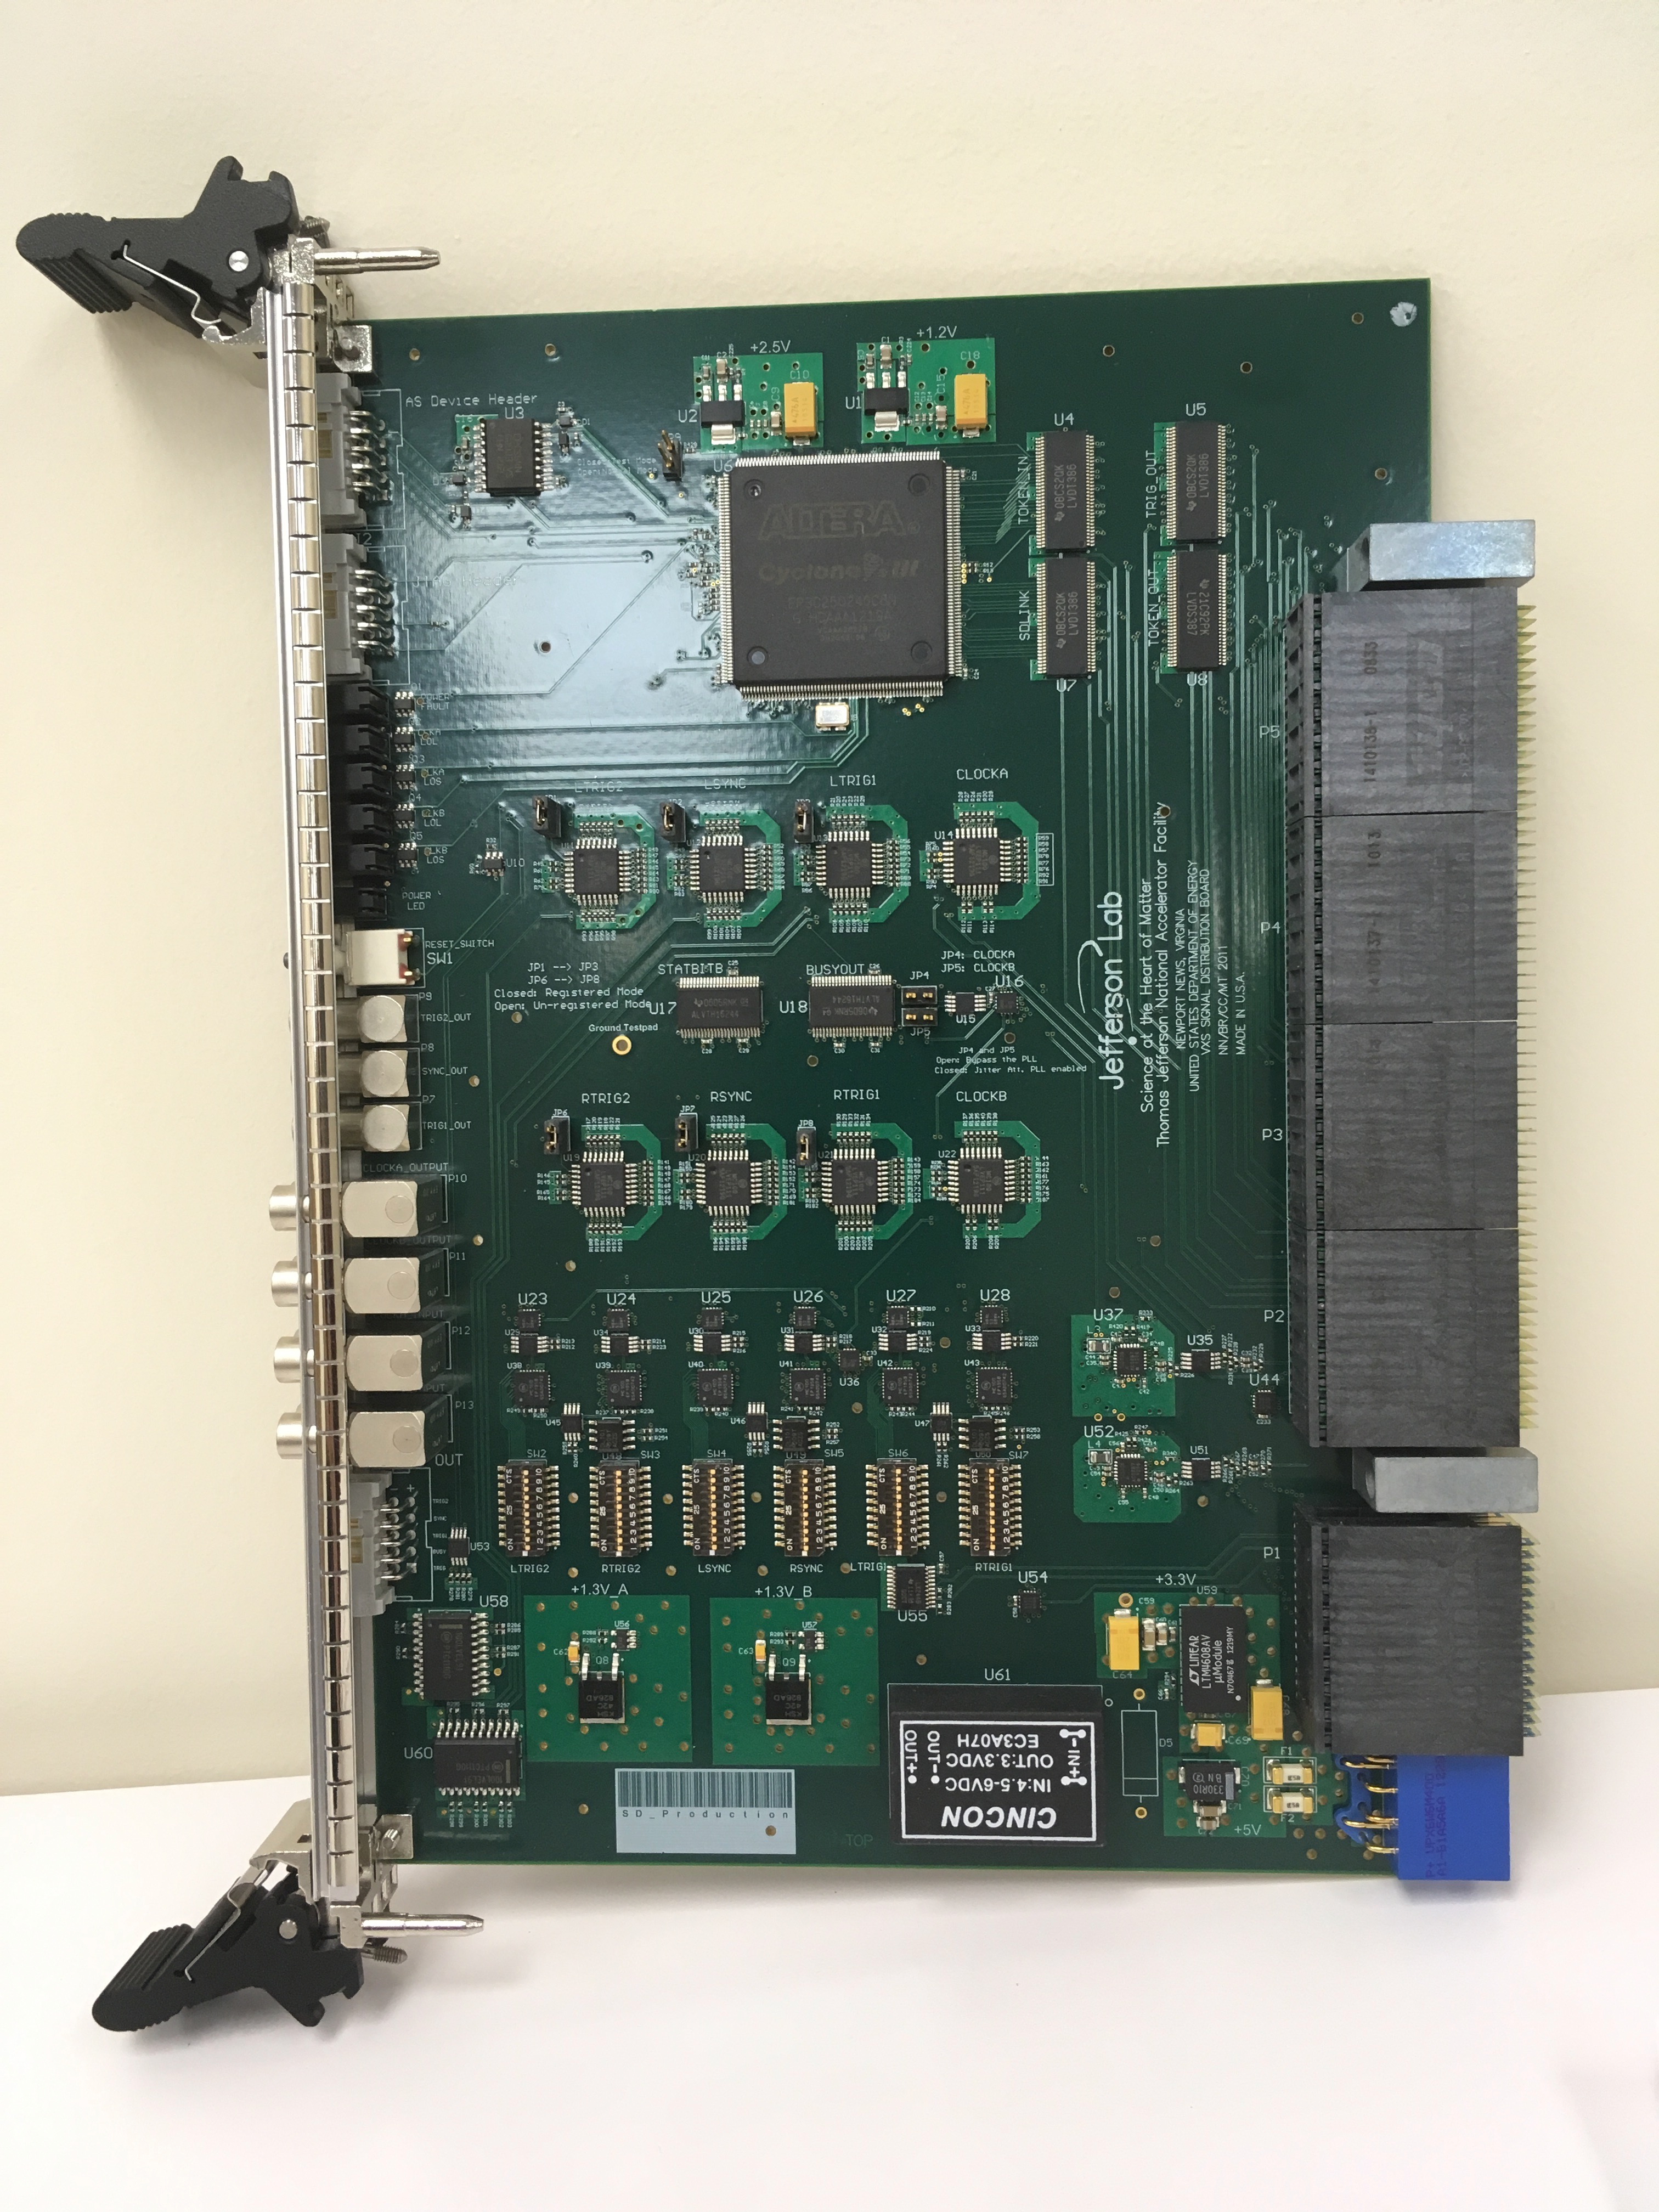
\includegraphics[width=1.0\columnwidth,keepaspectratio]{img/sd_board.jpg}
	\caption{Signal Distribution module (SD)}
	\label{fig:SDpic}
\end{figure}


\subsection{Flash ADC Module (FADC250)}

A 16-channel 250 MSPS pipelined flash ADC (FADC \cite{fadc-ref}, see Fig.~\ref{fig:FADC250pic}) with 12-bit precision was designed to digitize and process detector pulses for experiments at JLab.  The FADC250 module (see Fig.~\ref{fig:FADC250_board}) conforms to the VITA-41 VME64x switched serial (VXS) standard.  Each channel of the module accepts input signals on a LEMO style coaxial connector and has three user-selectable ranges (0.5 V, 1.0 V, 2.0 V).  Differential signal conditioning scales the input signals to within the dynamic range of the ADC and a single-pole low pass filter limits the signal bandwidth to the Nyquist band of the converter (125 MHz). Individual channel offsets are accomplished by means of DACs under VME control.  Each channel has its own dedicated ADC chip (Analog Devices AD9230). Both positive and negative polarity input signals are supported. The 250 MHz clock is distributed to the ADC chips through a low jitter ($<$ 2~ps) network.  

\begin{figure}[hbt]
	\centering
	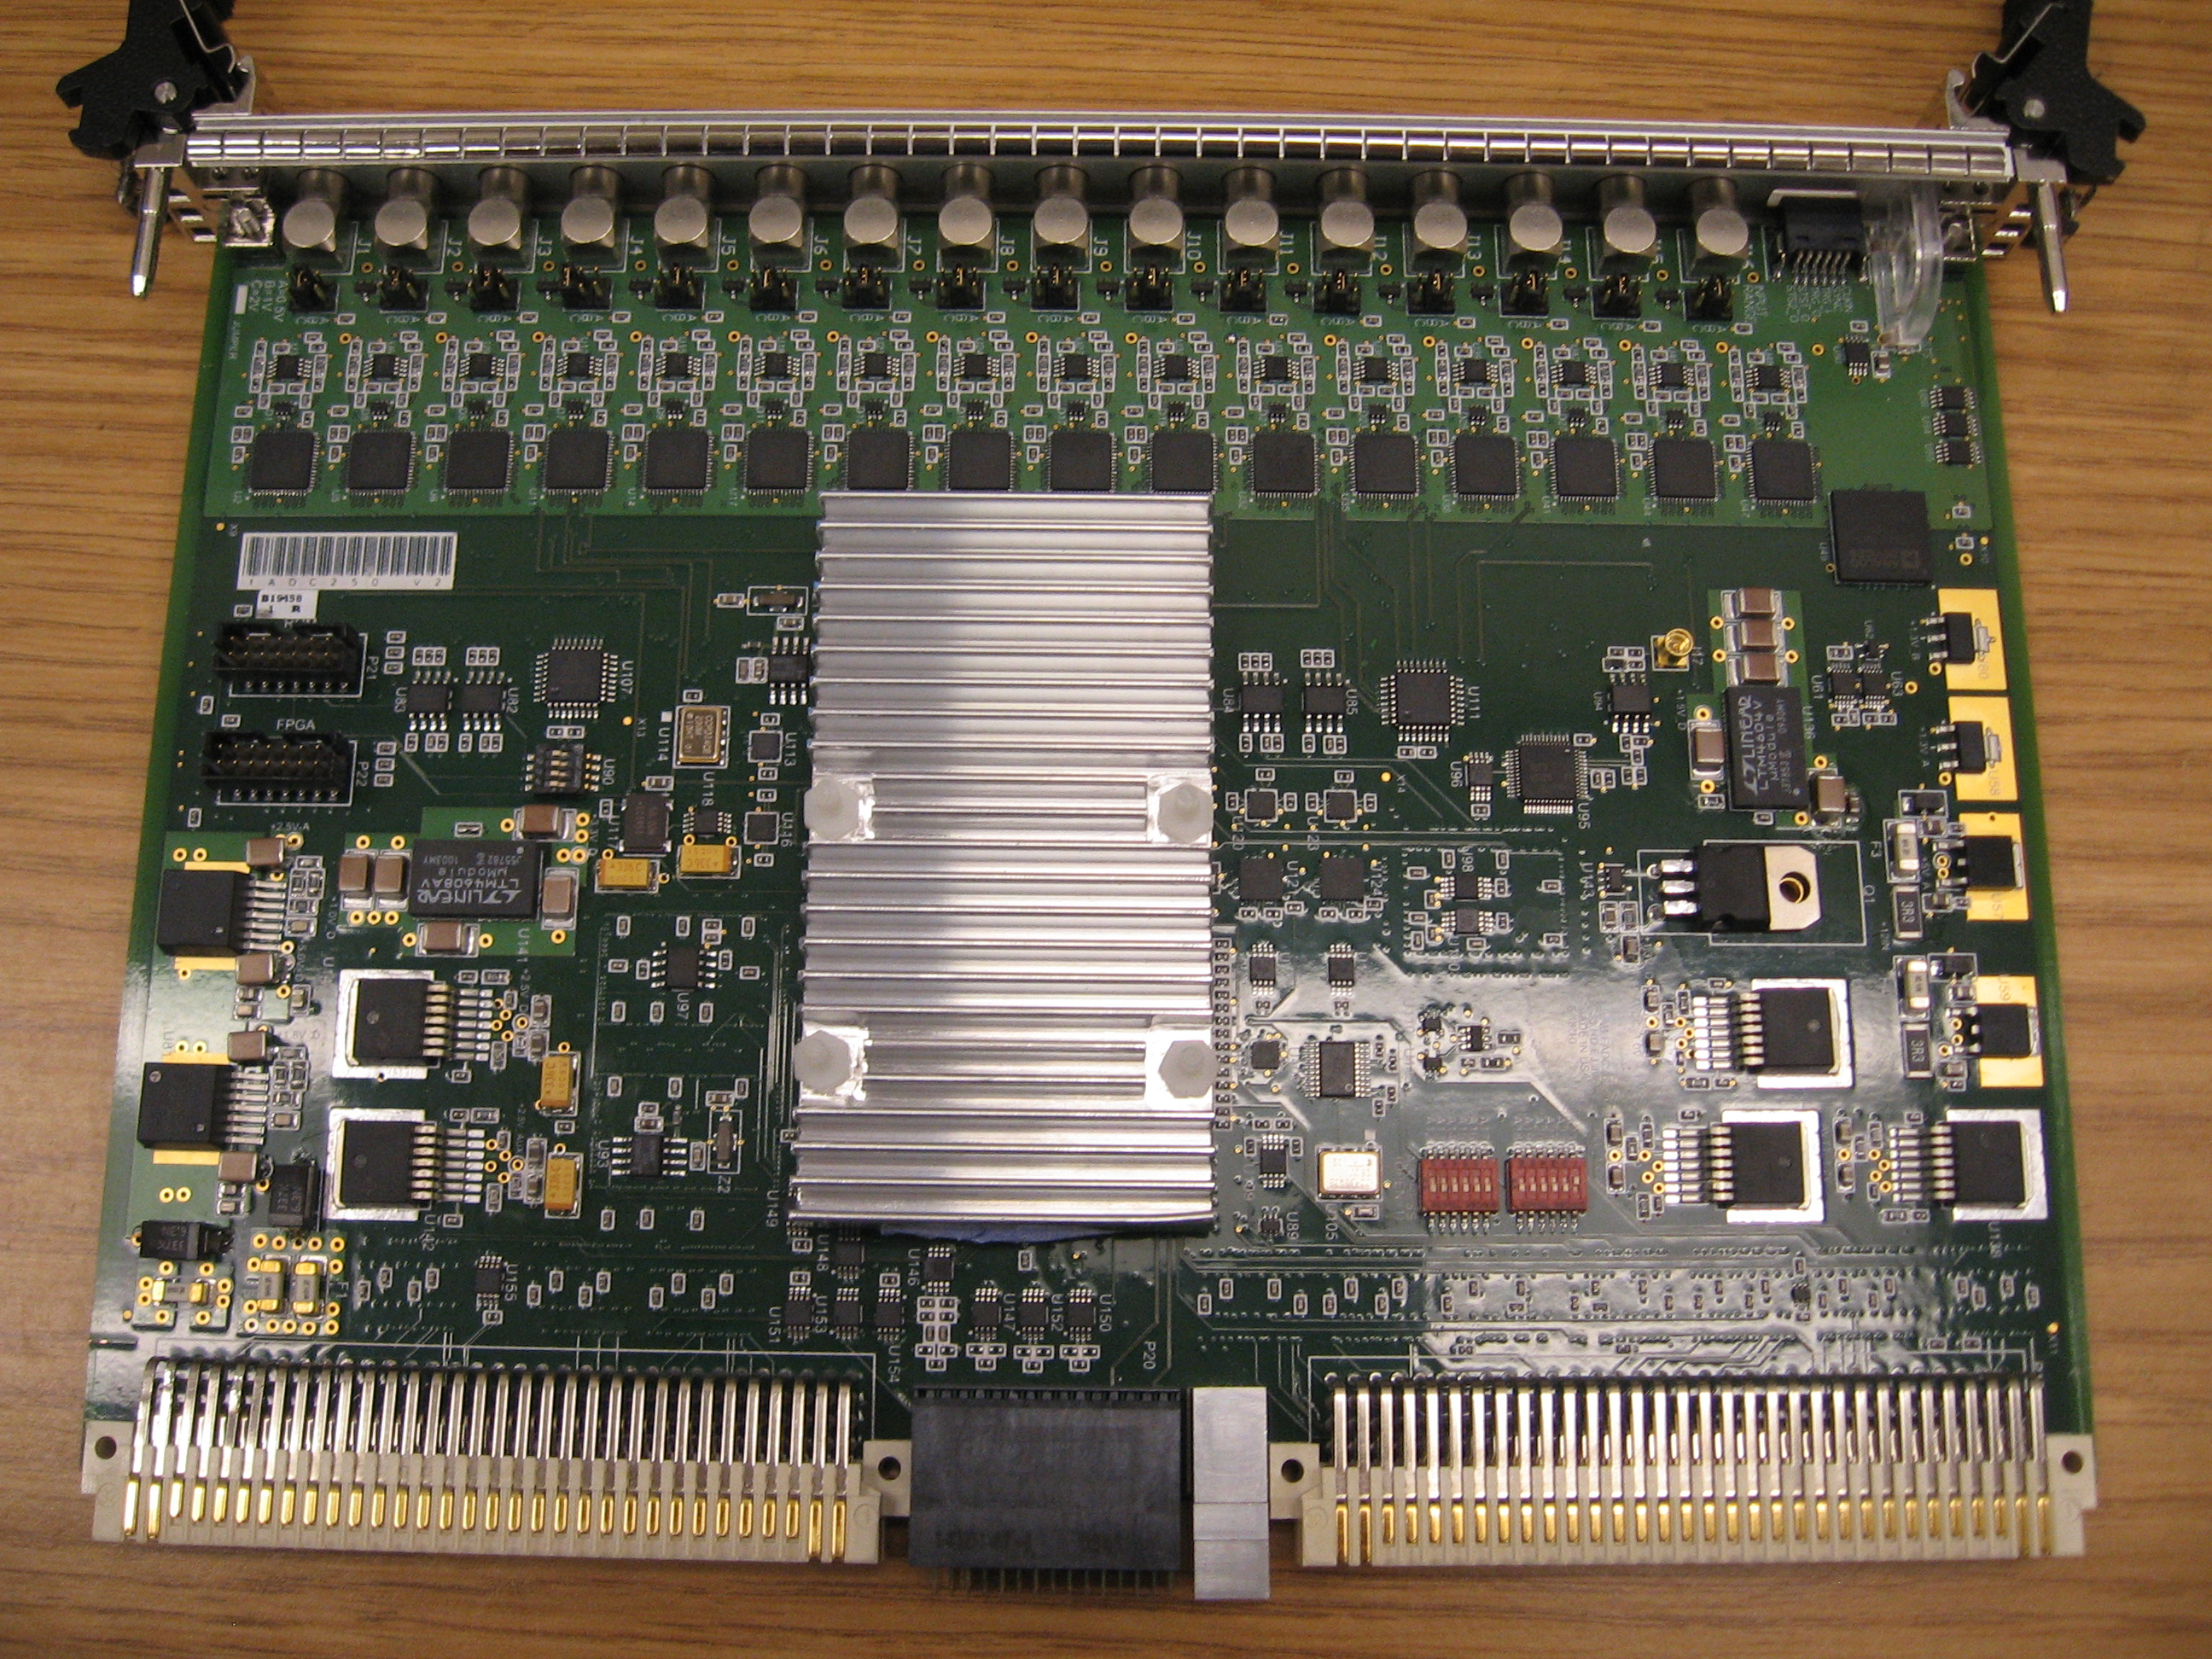
\includegraphics[width=1.0\columnwidth,keepaspectratio]{img/FADC250pic.jpg}
	\caption{Flash ADC module (FADC250)}
	\label{fig:FADC250pic}
\end{figure}

\begin{figure}[hbt]
	\centering
	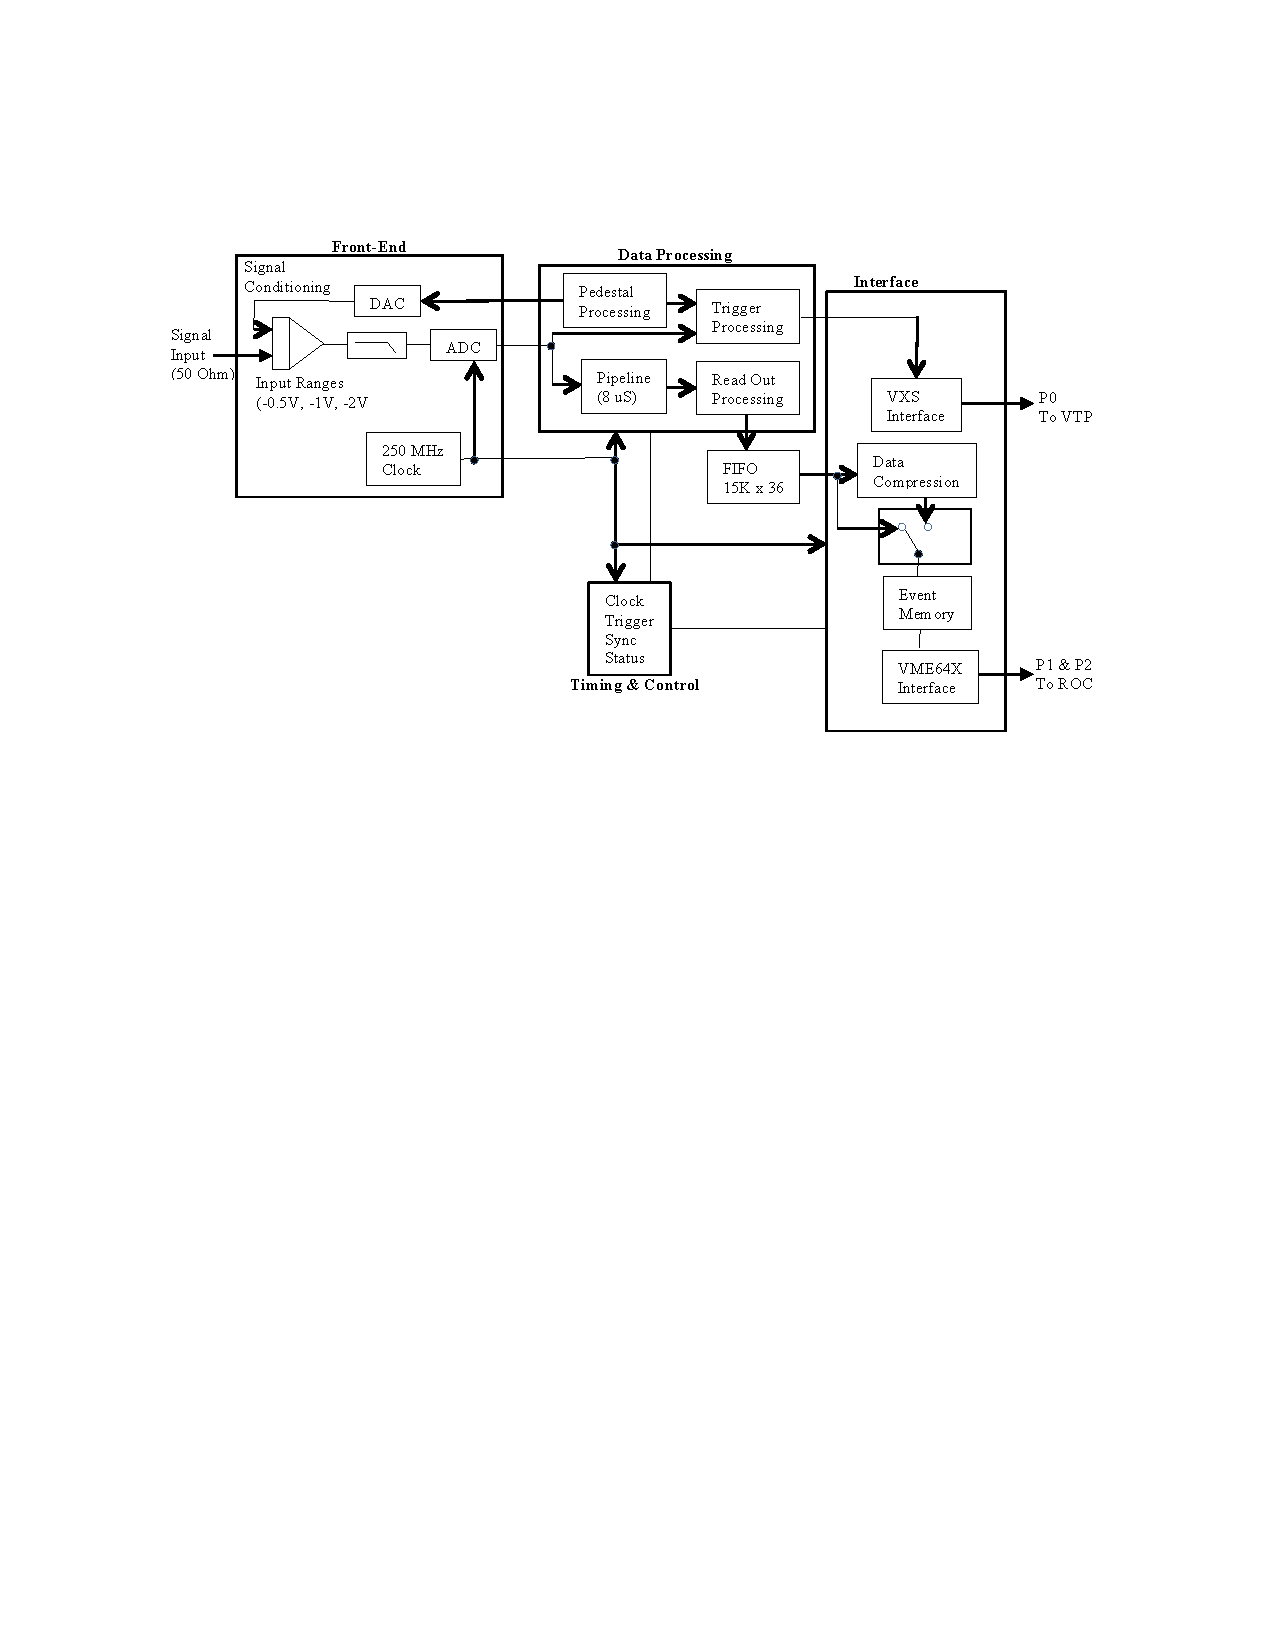
\includegraphics[width=1.0\columnwidth,keepaspectratio]{img/FADC250_Diagram.pdf}
	\caption{Flash ADC module diagram (FADC250)}
	\label{fig:FADC250_board}
\end{figure}

Digitized data from the 16 FADC chips is processed and formatted for readout in a pair of high performance Xilinx FPGAs. The digitized data from the ADCs follows two distinct paths.  Logic in the trigger data path pre-processes data for the trigger algorithms of the VXS Trigger Processor (VTP). The FADC250 module continuously streams this data to the crate VTP located in VXS switch slot A via high-speed serial links of the VXS fabric.  Data from multiple VTPs and other modules are used to form a global trigger signal that is returned to the crates to initiate data readout.

The readout data path continuously stores digitized data for each channel in circular buffers. When a trigger signal is received by the module a programmable window up to 2 $\mu$s wide of digitized data is extracted from the buffers for processing. The starting point of this window can be programmed up to 8 $\mu$s earlier than the arrival of the trigger signal to account for the time required to form the trigger signal.  Zero suppression on the extracted data may be implemented for each channel using programmable thresholds.  A lossless data compression algorithm can also be applied to the data of each channel with typical compression factors of 2 to 3. The design is pipelined so that data from multiple triggers can be processed simultaneously.  Triggers separated in time by as little as 50 ns can be accepted by the module. The trigger number and trigger time (clock periods since last synchronization) are reported along with the channel data so that data from multiple modules can be correctly assembled into events. 

Data associated with a programmable number ``N'' of triggers is packaged into a block of data for read out over VME.  ``N'' can take values from 1 to 255, with 40 being a typical value chosen.  Data is stored in an on-board 8 MB SRAM as 64-bit words to match the 64-bit high-speed (200 MB/s) dual edge VME Source Synchronous Transfer (2eSST) mode employed to read out the module.  

In order to save the overhead of setting up a DMA transfer for each FADC250 module in the crate, a chained block readout mechanism with token passing is used.  A common address range is enabled for all modules in the crate but only the module having the token will respond to a read request.  A single logical DMA read is initiated by the VME crate controller and the first module in the chain supplies data from its block of event fragments.  When the block data from the first module is exhausted, a token signal is passed to the next module in the chain and this module then proceeds to transmit its data from its block.  When the block for the data from that module is exhausted, it transfers the token to the next module.  This continues until the data from the last module in the chain is exhausted.  Instead of passing the token the last module asserts the VME bus error signal (BERR), which terminates the DMA cycle.  The user returns the token to the first module and the process can begin again when the next block of events is ready for readout.  The user does not have to query the modules in advance to discover the number of words to read out.  The DMA is set up with a total number of words larger than any expected value for the entire crate.  Data from each module is tagged with the slot number to identify its source.  The token passes along a VXS signal line to VXS switch slot B, where a module there (SD) routes it to the next enabled module.


\subsection{Discriminator Scaler Module (DSC2)}

The Discriminator Scaler Module (DSC2 \cite{dsc2-ref}, see Fig.~\ref{fig:dsc2_board}) is a 16-channel general purpose discriminator and scaler module designed as a 6U VME card. It replaces an older design, improving on jitter, noise, crosstalk, and adding new features.

\begin{figure}[hbt]
	\centering
	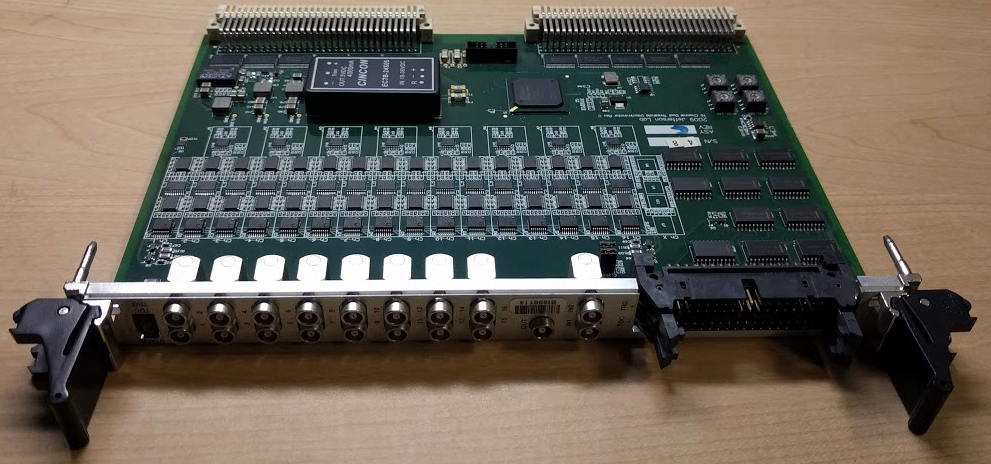
\includegraphics[width=1.0\columnwidth,keepaspectratio]{img/dsc2_board.png}
	\caption{Discriminator Scaler module (DSC2)}
	\label{fig:dsc2_board}
\end{figure}

\begin{center}
	DSC2 Specifications\\
	\begin{tabular}{| l | l |}
		\hline \hline
		Property			& Value				\\
		\hline
		{\bf Analog Discriminator}	&				\\
		Threshold			& 0 to -1023 mV			\\
		Pulse width			& 4 ns to 40 ns			\\
		Dead-time			& 4 ns typ. w/8 ns pulser width	\\
		Maximum input rate		& $>$125 MHz 			\\
		Ch-ch isolation			& $>$65 dB			\\
		Threshold noise			& 1.3 mV RMS (typical)		\\
		Slew-rate delay disperson	& $<$20 ps			\\
		Input-to-output delay		& $<$5 ns			\\
		{\bf Digital Processing}	&				\\
		Digital delay step		& 4 ns				\\
		Digital delay maximum		& 1 us				\\
		Digital width maximum		& 1 us				\\
		Maximum count rate		& 125 MHz			\\
		\hline \hline
	\end{tabular}
\end{center}

\paragraph{Discriminator}
Inputs are single-ended LEMO and leading-edge discrimated by two different thresholds. Typically one threshold is used for time-to-digital applications and the other threshold is used for trigger applications. There are separate differential ECL outputs for each channel and threshold. Low jitter performance was an important goal of the design as this module will be used in high resolution applications. Fig.~\ref{fig:dsc2_jitter} shows the typical jitter as a function of a variety of input slew rate signals and threshold overdrive conditions.

\begin{figure}[hbt]
	\centering
	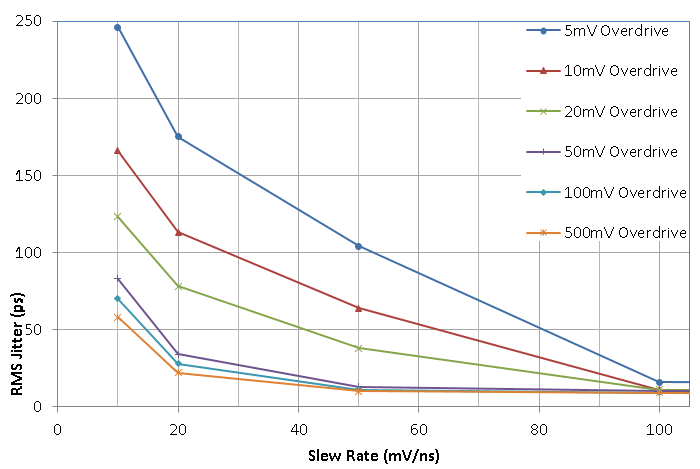
\includegraphics[width=1.0\columnwidth,keepaspectratio]{img/dsc2_jitter.png}
	\caption{Output Jitter vs Input slew rate and overdrive}
	\label{fig:dsc2_jitter}
\end{figure}

\paragraph{Digital Processing}
A Xilinx Spartan 3A FPGA is used to implement the VME interface, scalers, discriminator controls, and scaler event building features. Each channel and threshold has two scalers associated with it. The first scaler counts all threshold crossings for the input. The second scaler is gated using a front-panel input source, which can be useful to computing dead-time of channels and many other applications. Additionally, reference scalers are accumulated (a gated and ungated version) that count the elapsed time, which can be used to normalize inputs scalers to Hz. All together there are 68 scalers, which can be slow to read over VME if using single-cycle transfers. An event builder is implemented that can synchronously read (and optionally clear) all scalers and build an event with this data. Over 100 events can be buffered and readout using the VME 2eSST protocol at 200~MB/s.


\subsection{TDC Modiles (v1190/v1290)}

Commercial CAEN V1190/V1290/V1290N TDC \cite{tdc-ref} boards are used for timing measurements in the PMT-based CLAS12 detectors (see Fig.~\ref{fig:v1190_board}). The V1190 has timing resolution about 100~ps and the V1290 about 35~ps. All boards installed in CLAS12 run on an external 250/6=41.666~MHz clock rather then internal 40~MHz clock. The use of a different clock required compensation table remeasuring and reloading.

\begin{figure}[hbt]
	\centering
	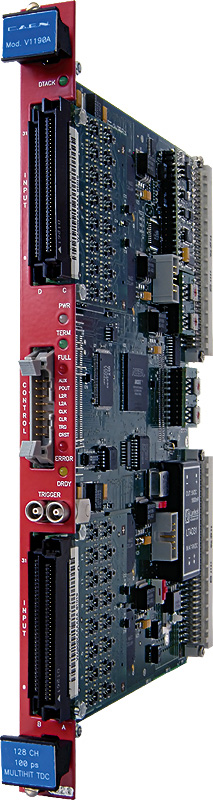
\includegraphics[width=0.2\columnwidth,keepaspectratio]{img/v1190_board.jpg}
	\caption{CAEN V1190 TDC module (V1190)}
	\label{fig:v1190_board}
\end{figure}

\subsection{Drift Chamber Readout Board (DCRB)}

\begin{figure}[hbt]
	\centering
	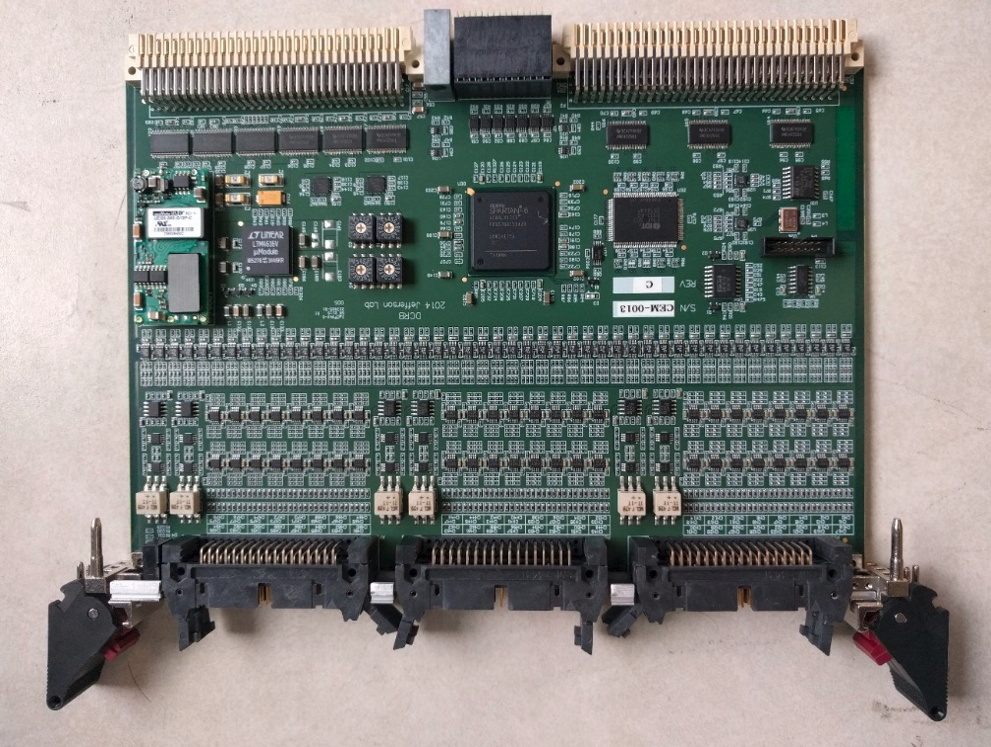
\includegraphics[width=1.0\columnwidth,keepaspectratio]{img/dcrb_board.png}
	\caption{Drift Chamber Readout Board (DCRB)}
	\label{fig:dcrb_board}
\end{figure}

The Drift Chamber Readout Board (DCRB \cite{dcrb-ref}, see Fig.~\ref{fig:dcrb_board}) is a 96-channel amplifier, discriminator, and time-to-digital converter module used to digitize and readout hits from the CLAS12 Drift Chambers. A single VXS crate of DCRB modules can readout a full region of the drift chambers for a single sector resulting in 18 VXS crates of DCRBs to instrument 6 sectors each having 3 regions of drift chamber.

\paragraph{Analog Inputs}
Each DCRB receives 96 differential analog signal pairs using twisted pair cabling from the drift chamber pre-amplifiers. The pre-amplfiers located on the detector provide a gain of ~2.3~mV/$\mu$A. On the DCRB each analog input channel is amplified by a voltage gain of 30 and then discriminated by a programmable threshold (common to all channels on the board with an effective chamber wire threshold range of 0 to 3.5/$\mu$A).

\paragraph{TDC Event Builder}
All discriminated channels go to a Xilinx Spartan 6 FPGA where a 96-channel 1~ns resolution time-to-digital converter (TDC) is implemented in firmware. The TDC is based on the ISERDES2 shift register FPGA primitive that directly samples of the digital input with a single-data-rate (SDR) input register clocked at 1~GHz. The TDC sampling clock is synchronized to the CLAS12 master oscillator, making it easy to relate hit times in the drift chamber to the other detectors in CLAS12. The TDC inputs are buffered to support multiple hits, allowing for an average hit rate of 4~MHz per input before loss of data, which exceeds the chamber design hits rates by a few orders of magnitude. Hits from groups of 16 channels are written into a large buffer that a linked-list content addressable memory (CAM) tracks for 16~$\mu$s. When a L1A trigger signal is received, a time window of hits is extracted from the TDC hit buffer. The readout window times are supplied to the CAM, and the CAM provides the address of the last hit matching each readout time bin. The hit buffer is then read to extract the hit and also the address of the next hit in the buffer matching the time bin (this is the linked list behavior). The result is an extremely fast event builder with natural zero suppression that does not require time sorted data. Cleanup is accomplished by a timer that invalidates the CAM entries after time bins are older then 16~$\mu$s. Hits for an event are assembled and buffered in a 2~MByte external RAM, which is readout through the VME bus using the 2eSST protocol at 200~MB/s.

\paragraph{Calibration Support}
A programmable amplitude pulse generator is implemented that can inject test pulses directly into the DCRB differential amplifier inputs as well as to the pre-amplfiers that are on the detector. This provides a way to test points of failure, check channel gain, and check channel delays without any extra equipment. A scaler is implemented on each channel for slow control monitoring of all chamber wires.

\subsection{VXS Silicon Readout Module (VSCM)}
The CLAS12 Silicon Vertex Tracker detector (SVT, \cite{svt-ref}) front-end utilizes the data driven FSSR2 ASIC for digitization. The VXS Silicon Readout Module (VSCM \cite{vscm-ref}, Fig.~\ref{fig:vscm_board}) was designed to interface the FSSR2-based front-end to the CLAS12 DAQ system. This system is capable of reading out all 33,792 SVT channels in 3 VXS crates.

\begin{figure}[hbt]
	\centering
	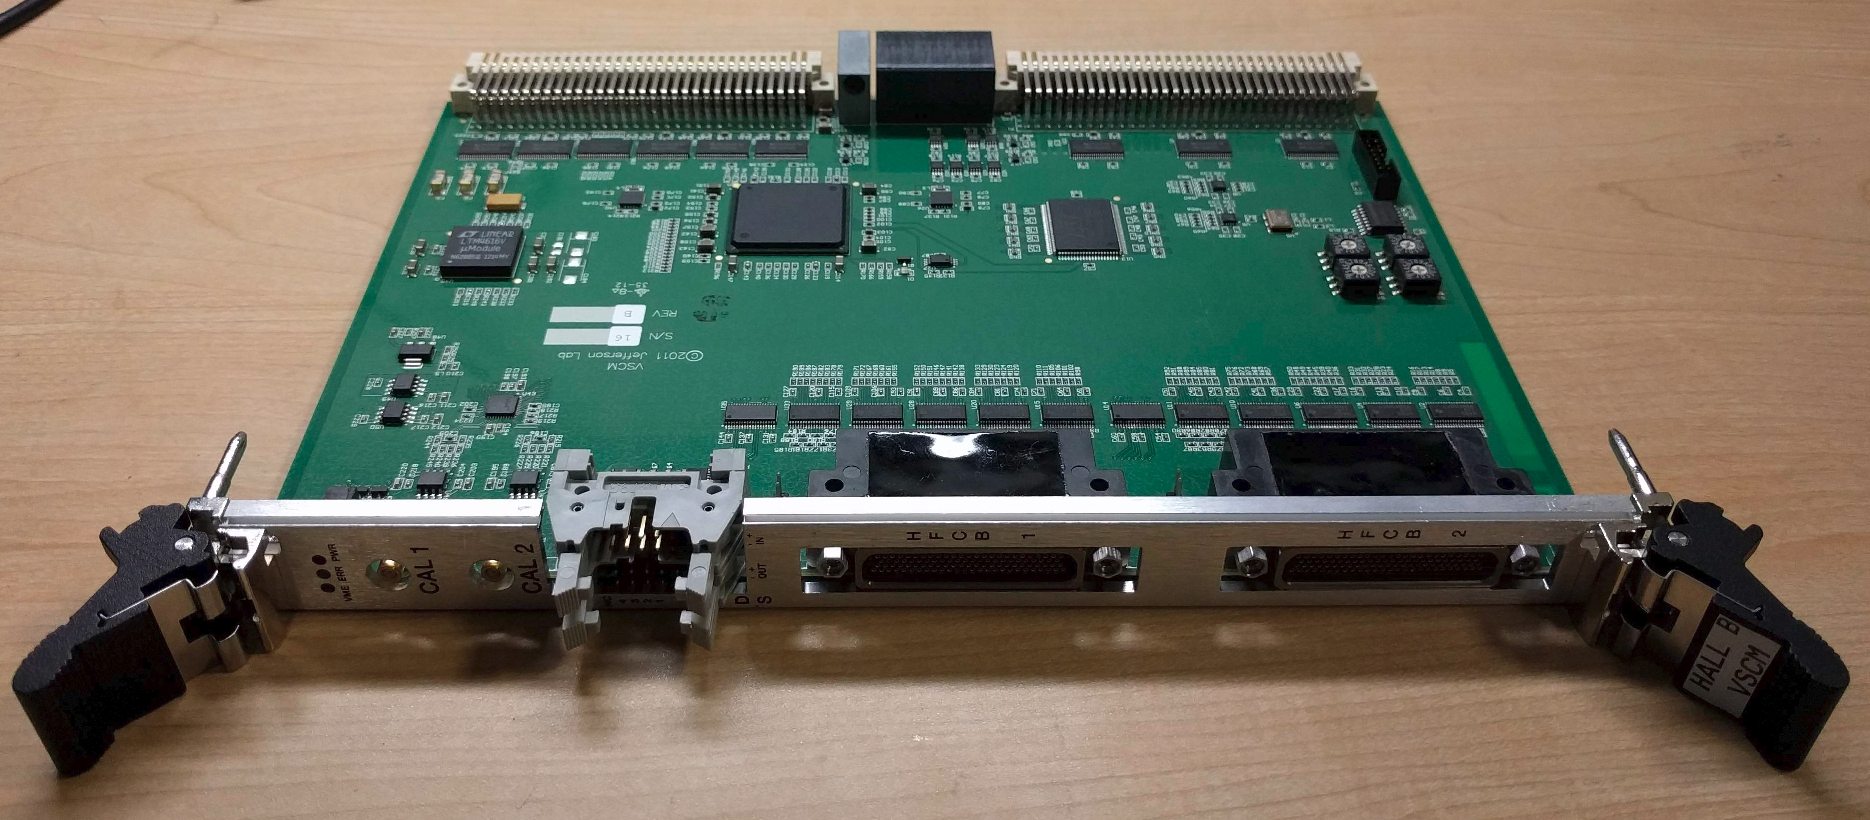
\includegraphics[width=1.0\columnwidth,keepaspectratio]{img/vscm_board.png}
	\caption{VXS Silicon Readout Module (VSCM)}
	\label{fig:vscm_board}
\end{figure}

The main features of the VSCM include:

\begin{itemize}
	\item Receives 8 FSSR2 streams, each at 840~Mbps
	\item De-randomizes hits into an 8~$\mu$s buffer
	\item 512k hit, multi-event buffer
	\item Supports $>$1~MHz trigger rate
	\item Programmable amplitude charge injector
	\item 1~ns resolution time-to-digital converter (TDC)
	\item Per channel hit scaler
	\item FSSR2 synchronization, status, and control
\end{itemize}

\paragraph{Event Builder}
The VSCM deserializes the FSSR2 streams, checks for errors, and decodes the hits, which are stored in an 8~$\mu$s circular memory. The hits are not guaranteed to be time ordered, so the timestamp and channel number are used to form the circular memory address (rather than storing in the order received). The VSCM also implements an 8-channel 1~ns time-to-digital converter (TDC) that measures the logic OR of hits from each FSSR2 ASIC. This high time resolution is significantly better than the FSSR2 serial stream hit time resolution and is required for improved out-of-time hit rejection. The L1A trigger signal time is used to look back a fixed amount of time and extract a time window of hits from the circular memory, which corresponds to the physics event. Non-zero hits are assembled as an event and buffered in a 2~MByte external RAM that is readout through the VME bus using the 2eSST protocol at 200~MB/s.

The event data contains primarily two hit word types that together provide high time resolution and spatial hit resolution while keeping the front-end complexity low.

\begin{center}
	Low time resolution hit word\\
	\begin{tabular}{| l | l |}
		\hline \hline
		Property	& Description		\\
		\hline
		Hit Time	& 128~ns resolution	\\
		Channel		& 0-1023 strip ID	\\
		Charge		& 0-7 threshold		\\
		\hline \hline
	\end{tabular}
\end{center}

\begin{center}
	High time resolution hit word\\
	\begin{tabular}{| l | l |}
		\hline \hline
		Property	& Description		\\
		\hline
		Hit Time	& 1~ns resolution	\\
		Channel		& 0-7 chip ID		\\
		\hline \hline
	\end{tabular}
\end{center}

Fig.~\ref{fig:vscm_blockdiagram} shows the hardware block diagram of the module. Essentially, a single low-cost Xilinx Spartan 6 FPGA was used to implement the deserialization, buffering, event-building, monitoring, front-end configuration, time-to-digital conversion, and monitoring.

\begin{figure}[hbt]
	\centering
	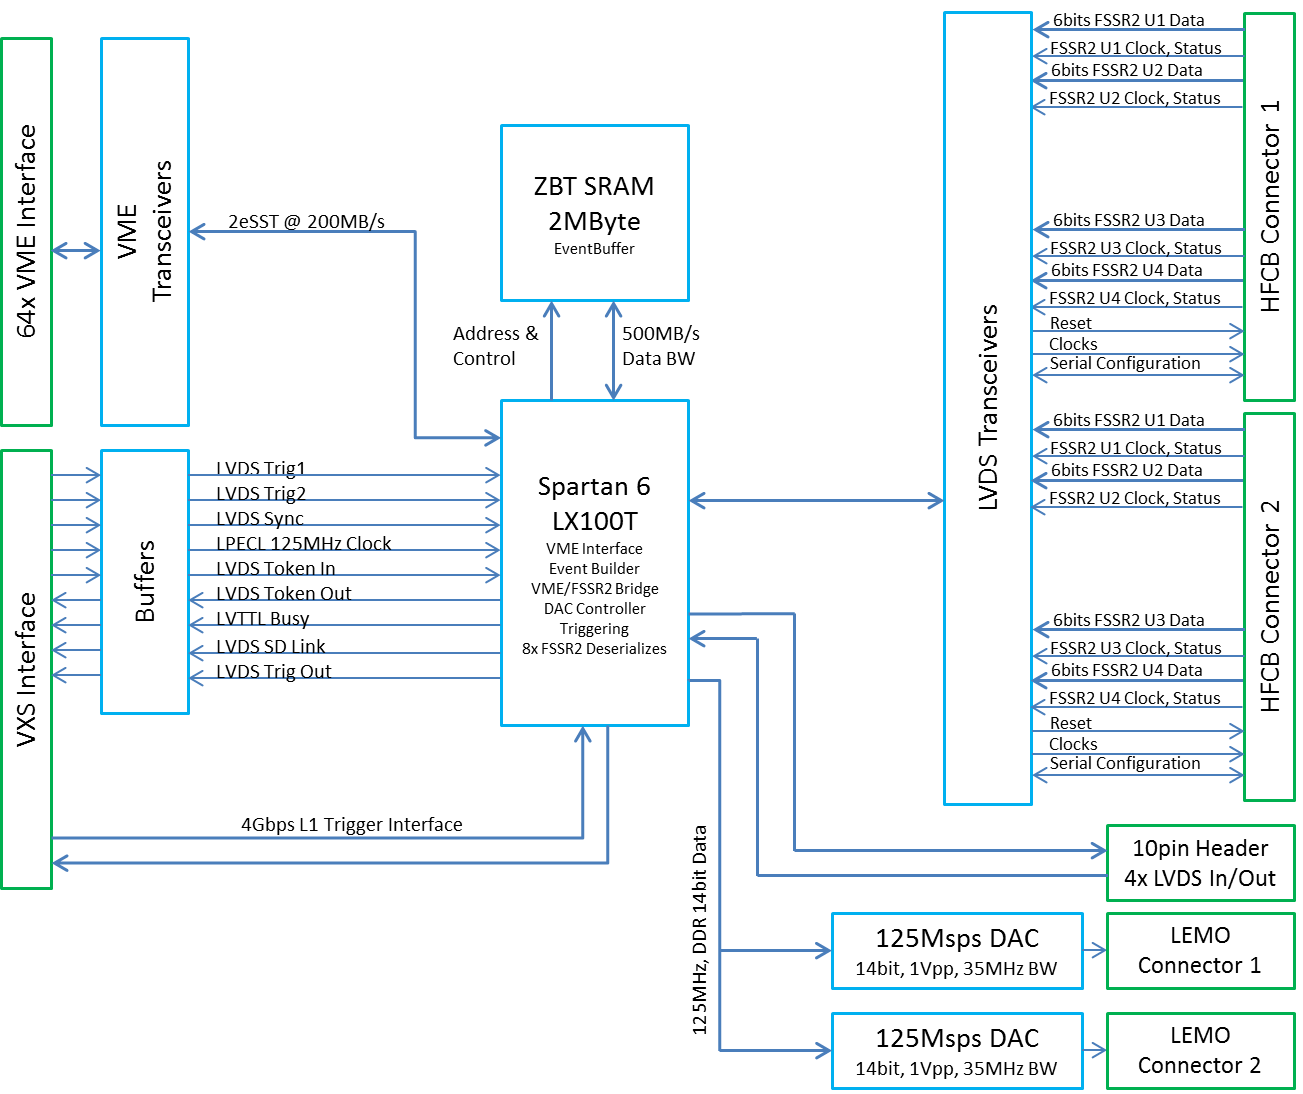
\includegraphics[width=1.0\columnwidth,keepaspectratio]{img/vscm_blockdiagram.png}
	\caption{VSCM Hardware Diagram}
	\label{fig:vscm_blockdiagram}
\end{figure}


\subsection{SSP Board as ffber Readout Module}

The SubSystem Processor (SSP \cite{ssp-ref}) was originally designed to work as part of CLAS12 Trigger System. It is used to readout some front-end electronics in the DAQ system as well. The board description can be found in the CLAS12 Trigger System article \cite{trig-ref}.
\section{Electronics}

The MVT data acquisition system is designed to read out 6,000 channels of the forward station and 18,000 channels of the
barrel station. With the physics background as high as 20~MHz, the strip hit rates are about 60~kHz and 20~kHz in the
forward detectors and in the barrel detectors, respectively. The readout system is compliant with the CLAS12 requirements
of a 20~kHz maximum trigger rate and provides a sufficiently long data pipeline to cope with up to 16~$\mu$s trigger decision
latency. Timing precision of a few ns is sufficient to limit the number of ghost hits compatible with the timing of the trigger
signals. A charge measurement with a 10-bit dynamic range is enough to cover the full span of the Micromegas detector signals
and to discriminate accurately minimum-ionizing particles (MIPs) from noise. Note that the FT-Trk uses the same readout electronics and architecture as the MVT.

\subsection{Readout System Architecture}

The extremely compact and dense design of the CLAS12 Central Detector leaves a very narrow space between the MVT and
its neighbor subsystems, as well as between the Micromegas detectors themselves.  In addition to the stringent space limitations, the
operational conditions of the tracker are harsh in terms of radiation and the high 5~T magnetic field. Keeping a low material budget
is an obvious concern. Consequently, a readout architecture based on off-detector front-end electronics has been adopted.
Lightweight micro-coaxial cable assemblies with low 40~pF/m linear capacitance carry bare, unamplified signals to the Front-End
Units (FEU) housed in crates $\sim$1.5--2~m upstream of the detectors. 

\begin{figure*}[htb]
\begin{center}
 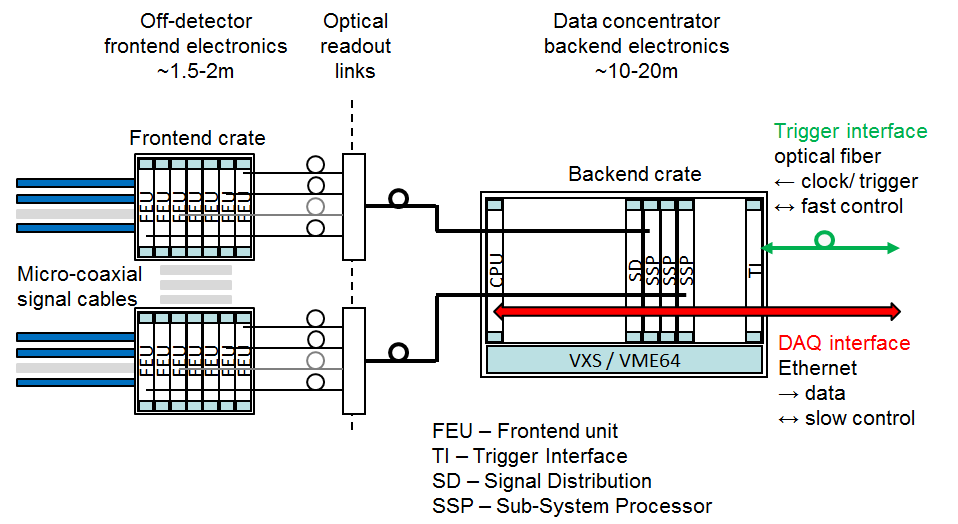
\includegraphics[width=1.6\columnwidth,keepaspectratio]{images/electronics_fig1.png}
\end{center}

 \caption{MVT and FT-Trck readout system.}
 \label{fig:mm-e_1}
\end{figure*}

The front-end electronics are responsible for the amplification and shaping of the detector signals, for holding the latter in a
pipeline waiting for a trigger signal, for the digitization and compression of the selected event data, and for their
delivery to the back-end electronics. The back-end is responsible for data concentration event by event. It provides an interface
with the CLAS12 event building system, ensures a fixed latency path between the CLAS12 trigger system~\cite{trigger-nim} 
and the FEUs, and receives the system clock and trigger from the CLAS12 trigger supervisor and synchronously conveys 
them to the FEUs over bidirectional optical links. A schematic representation of the readout system architecture is 
shown in Fig.~\ref{fig:mm-e_1}.

\subsection{The 64-Channel DREAM ASIC}

Depending on the type and size of the CLAS12 Micromegas detectors, the strip capacitances vary from 60 to 120~pF. The total
capacitance seen by the front-end electronics input is even higher, up to 200~pF due to the contribution from the detector
micro-coaxial cables. To achieve a comfortable signal to noise ratio (SNR) well above 10, the equivalent noise charge (ENC) of the
detection chain should be $\sim2500~e^-$ for the $140-200$~pF range of the total input capacitance. At the time of the
detector development, no existing ASICs could deliver the required performance while, in addition, sustain the 20~kHz readout
rate and provide the 16$~\mu$s deep trigger pipeline required. A new 64-channel ASIC, called DREAM (for Dead-timeless
Readout Electronics ASIC for Micromegas), has been developed~\cite{DRM}. 

\begin{figure*}[htb]
\centering
 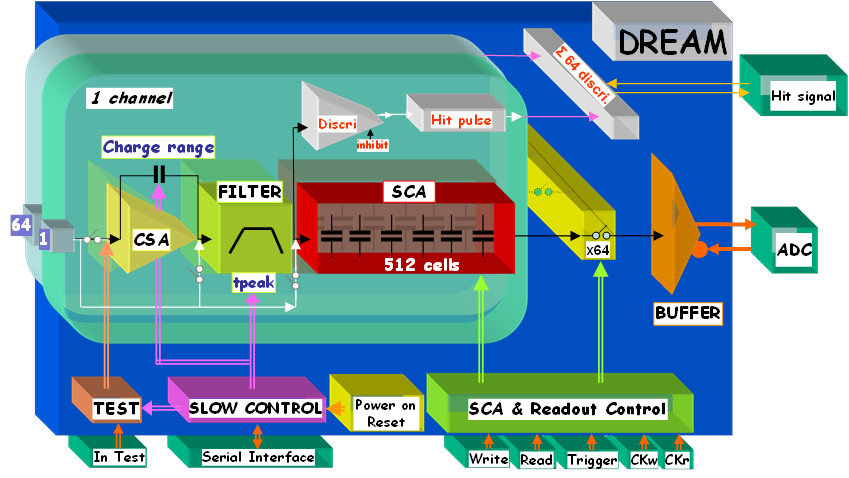
\includegraphics[width=.8\textwidth,keepaspectratio]{images/electronics_fig2.png}
 \caption{Block diagram of the DREAM ASIC.}
 \label{fig:mm-e_2}
\end{figure*}

The DREAM ASIC block diagram is shown in Fig.~\ref{fig:mm-e_2}. Each channel includes a charge sensitive amplifier 
(CSA) adapted to a wide spread of detector capacitances (up to 1~nF) and
four selectable charge measurement ranges (from 50 to 600~fC), a shaper with programmable peaking times (from 75~ns to
1~$\mu$s), and 512-cell deep Switched Capacitor Array (SCA) used as the trigger pipeline memory and a de-randomization buffer.

The input signals are continuously sampled and stored in the SCA at a rate of up to 50~MHz. Upon reception of the trigger signal,
a programmable number of samples of all channels, corresponding in time to the event, is read out serially through a differential
analog buffer capable of driving an external ADC at a frequency of up to 28~MHz. The sampling is not stopped during the readout
process, which allows nearly dead-timeless operation. Other features, such as the ability to operate with both signal polarities,
the possibility to inject input signals directly into the SCA memory bypassing the filter and/or CSA, and integrated per-channel
discriminators (useful to form trigger primitives), make the chip extremely versatile. The integrated circuit is manufactured in
the AMS CMOS 0.35~$\mu$m technology and is encapsulated in the 128-pin LQFP square package with a 1~mm side and a
0.4~mm pitch.

\subsection{The 512-Channel Front-End Unit (FEU)}

The FEU is a mixed analog-digital electronics board. The analog section comprises eight input connectors, protection circuits,
DREAM ASICs, and an 8-channel flash ADC (see Fig.~\ref{fig:mm-e_3}). The protection circuits are optional.  They are installed
on the FEUs to protect the DREAMs from the sparks of the standard Micromegas detectors. When working with resistive
detectors, the input channels of the DREAM ASICs can be directly connected to the detector strips, improving the signal to
noise ratio. The protected or non-protected type of FEUs are determined during their manufacturing.

\begin{figure}[htb]
 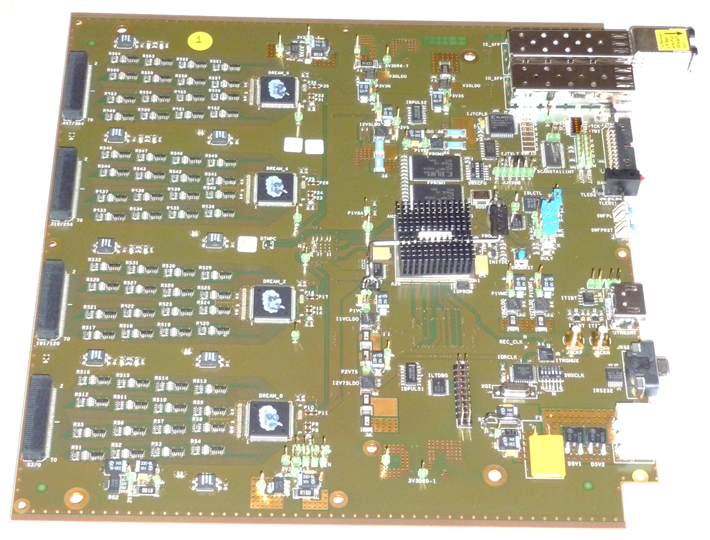
\includegraphics[width=1.0\columnwidth,keepaspectratio]{images/electronics_fig3.png}
 \caption{Photograph of the 512-channel Front-End Unit.}
 \label{fig:mm-e_3}
\end{figure}

As described above, the pre-amplification, shaping, and trigger pipeline functionality is implemented in the DREAM chips. The
analog samples from the eight DREAMs are digitized by an 8-channel 40~MHz 12-bit flash ADC AD9222 from Analog Devices
\cite{ADC}. The eight serial streams of digital data are delivered to the on-board FPGA. The digital section of the board
comprises an xc6vlx75t-2-ff748 FPGA from the Xilinx Virtex-6 device family~\cite{XIL}, its configuration memory, a 2~Mbyte
synchronous SRAM, small form-factor pluggable (SFP) transceivers, an on-board clock synthesizer, and an auxiliary trigger
interface circuit.

The FPGA controls the DREAM integrated circuits and the ADC, producing the sampling and readout clocks, as well as various
required control signals. One of the SFP cages is populated with an optical transceiver module that is used to establish a
synchronous communication channel with the back-end electronics over a 2.5~Gbit/s link. In the downstream direction, the link
encodes the 125~MHz system clock, trigger signals, and fast synchronous commands.

Upon accepting the trigger signal, the FPGA reads the corresponding samples from the DREAMs and optionally applies the
following digital data processing steps. First, after serial to parallel conversion, the pedestals are equalized. Next, for each
sample, the coherent noise affecting the DREAM inputs is estimated and subtracted on a chip-by-chip basis. This greatly
improves the noise immunity of the MVT readout system. Finally, the per-channel zero suppression is performed. The retained
samples describe the signal development in the channel. Fitting their values with a known function allows an accurate estimation of
deposited charge and of signal timing. For each accepted trigger, the FPGA forms an event fragment from the retained channel
data and delivers it to the back-end electronics via the optical channel. The optical channel is also used for setting and monitoring
the run control parameters.

The FEU is a 6U (266~mm) high, 220~mm deep, and 5HP (25.4~mm) wide module. The thickness of its 12-layer PCB is 1.6~mm. It
can be powered from either a 4.3~V or 5~V source and consumes slightly less than 20~W when all eight DREAMs operate in their
most power-hungry mode. The FEUs have been operated in a magnetic field of up to 1.5~T without any perceptible change of their
power consumption or functionality.

\subsection{The Back-End Unit (BEU)}

The back-end of the data acquisition system of the MVT is based on the JLab standard VME/VXS hardware including a trigger
interface (TI), a signal distribution (SD) and a sub-system processor (SSP) board, and a crate controller single board computer
(SBC)~\cite{daq-nim}. The flow of the trigger, data, and control messages is shown in Fig.~\ref{fig:mm-e_1}. 

% \begin{figure*}[htb]
% \begin{center}
%  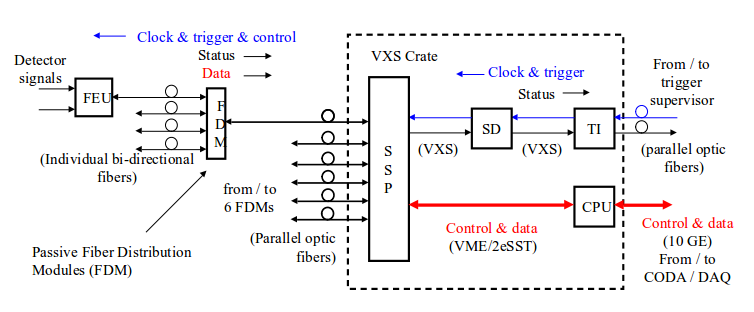
\includegraphics[width=1.6\columnwidth,keepaspectratio]{images/electronics_fig4.png}
% \end{center}
% 
%  \caption{MVT back-end unit and dataflow.}
%  \label{fig:mm-e_4}
% \end{figure*}

The TI receives a low jitter 250~MHz system clock and fixed latency trigger signals from the CLAS12 trigger supervisor. It
also delivers to the trigger supervisor the status information (e.g. busy) of the MVT readout system. The physical layer interface
is based on a parallel optic technology. The clock and trigger signals are delivered to the SD board over the VXS backplane. The
SD board conveys properly delayed and aligned clock and trigger signals to the SSP boards. It also gathers their status
information, and then combines and sends it to the TI board. These communications happen over the VXS backplane.

The SSP board was primarily designed to be a part of the hardware level trigger logic of the JLab experiments. Given the
massive resources it provides (notably a Virtex-5 TX150T Xilinx FPGA, 32 multi-gigabit transceivers (GTX) routed to the
front panel, 4 Gbyte DDR2 memory), it was considered for the readout of the MVT front-end electronics. The SSP firmware
has been modified to fit the needs of the MVT Back-End Unit (BEU).

An SSP can distribute the global system clock, trigger, and synchronous commands to up to 32 FEUs. In practice, there are
two Back-End Units each serving 24 front-ends. The trigger pulses and fast run control commands are broadcast synchronously
to all FEUs over the synchronized fixed latency 2.5~Gbit/s links. The protocol between the FEUs and the BEU sets an 8~ns
resolution on successive triggers and synchronous commands (125~MHz clock). However, the dispersion of their arrival times
on the FEUs is well under 1~ns.

On each trigger, the SSPs time stamp the event with the synchronous 125~MHz clock and assign it the event counter value. The
48-bit time stamp along with the 60-bit event identification (ID) is used for local event building. This process implies gathering from all FEUs
the event data packets belonging to the same event (matching time stamps, and event IDs). Multi-event buffers, with a
programmable number of events, are constructed in the external DDR2 memory. Upon the request from the crate controller
SBC, the contents of the buffers are transferred to its memory over the VME64 backplane using the 2SST protocol. Transmission
rates of $\sim$200~Mbyte/s are routinely achieved.

The SBC executes the data collection and the run control tasks within the CODA software framework~\cite{daq-nim}. It 
also
completes the data integrity checks performed in the SSP firmware, disentangles multi-event buffers, forms MVT events
concatenating the FEU/SSP data with the corresponding TI data, and sends them to the CLAS12 Event Builder over a 10~GB/s
Ethernet link.

The MVT readout electronics is continuously monitored by the CLAS12 detector monitoring system using the EPICS framework.

\section{Calibration}

Since the SVT modules are designed with a binary readout system, the analog channel response cannot be measured directly. Instead, the analog response is reconstructed by injecting a calibration charge on the channel and measuring the corresponding occupancy over a range of threshold values. 

\begin{figure}[hbt] 
	\centering 
	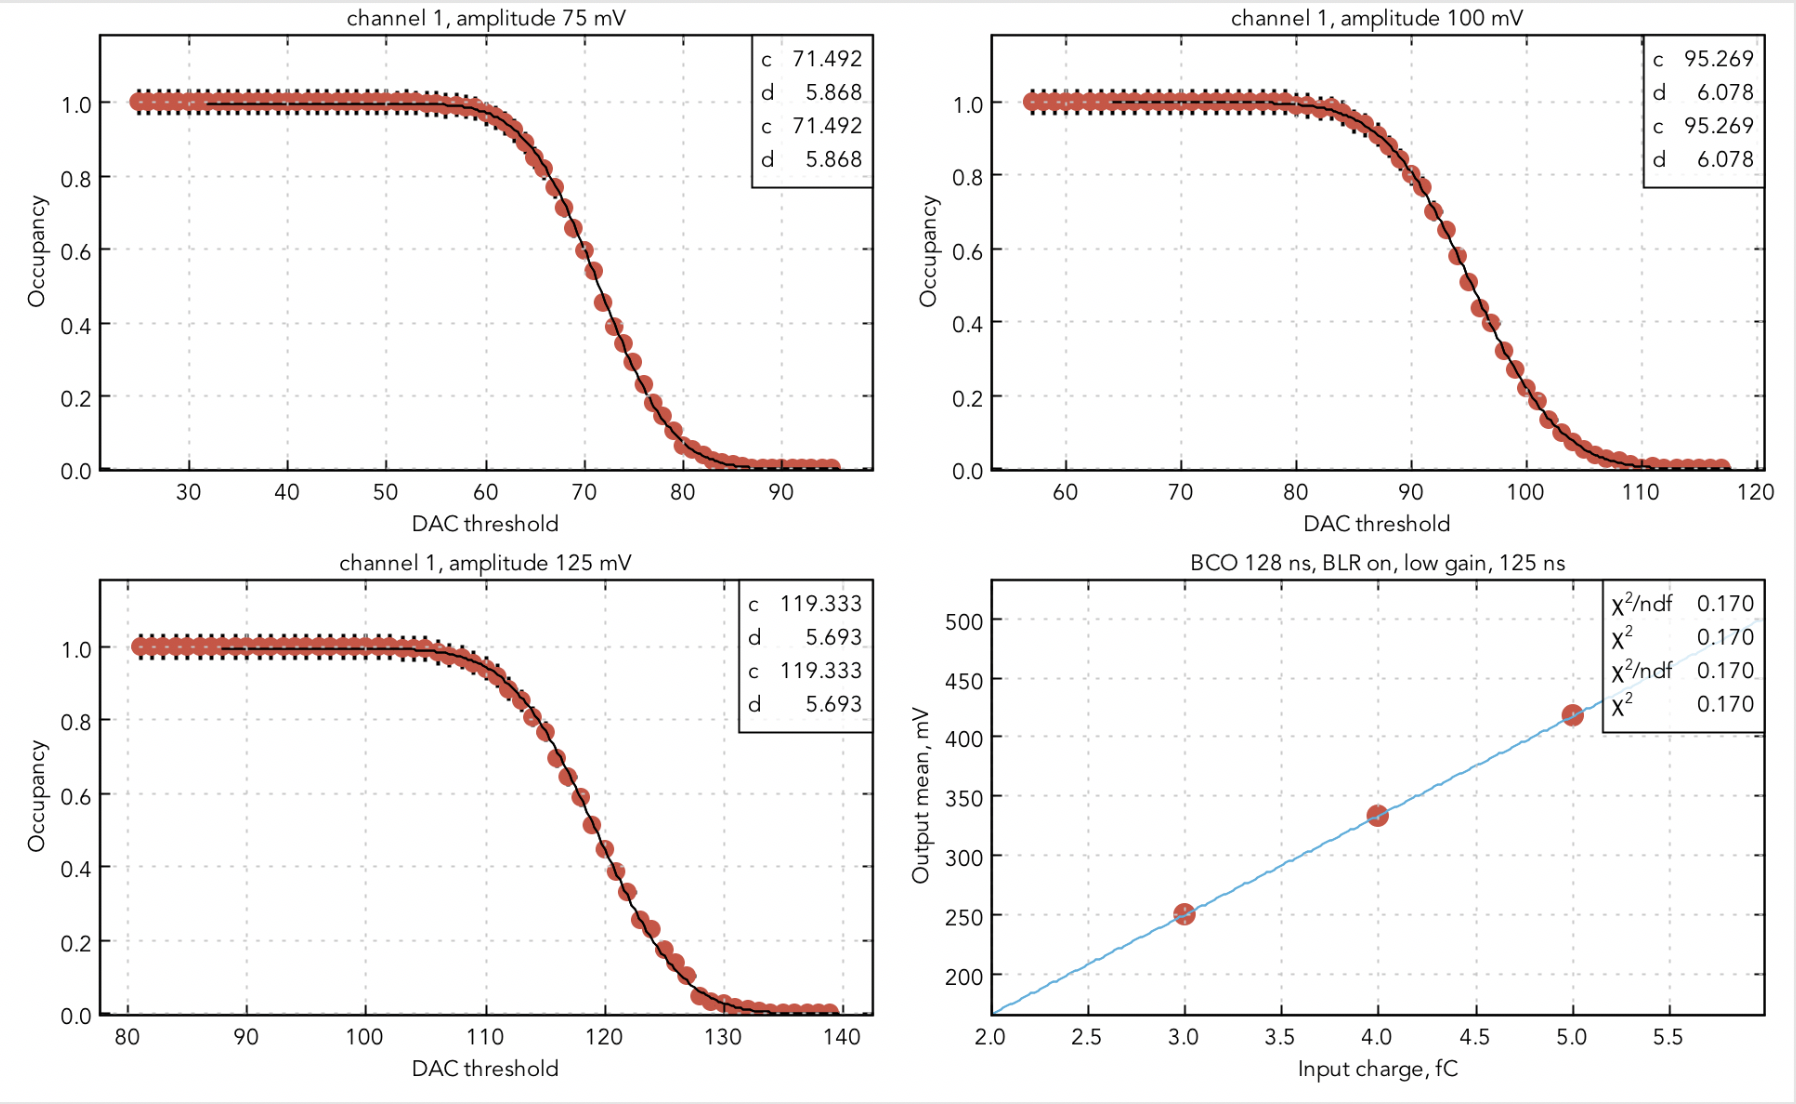
\includegraphics[width=1.0\columnwidth,keepaspectratio]{threshold-scan.png}
	\caption{Threshold scan on a single representative SVT channel.}
	\label{fig:threshold-scan}
\end{figure}

The output signals from the FSSR2 chip can be converted to charge using either internal or external calibration pulses. Because external pulser can be set to higher frequency than internal pulser without affecting the calibration process, external pulser circuit was added to the HBCB and the VSCM. Noise is measured using external, low frequency calibration charge injected in the absence of signal. The injected charge is shaped and amplified in the analog circuitry to form an output signal. The discriminator threshold determines whether or not the output signal corresponded to a hit. The probability that the injected charge produces a hit depends on the setting of the discriminator threshold. The average hit probability is measured by repeating the process of injecting charges and counting the fraction of readout triggers that produced a hit. This measurement is repeated over a range of threshold settings to produce an occupancy plot. 

The occupancy plots are measured setting the pulser amplitude at fixed values and changing the comparator thresholds. Each point of an occupancy plot represents the percentage of times that the comparator fires for a certain value of injected charge. In Fig.~\ref{fig:threshold-scan} presented three occupancy plots taken at different pulser amplitudes and the response plot showing the linear dependence of the output pulse height on the input charge in the operation region of the preamplifier. In between the high and low threshold regions, the occupancy curve is described by an error function, or S-curve, which can be fitted to the occupancy histogram for each channel, producing a mean value (discriminator threshold) and standard deviation (noise). The conversion from mV to electrons is performed considering a nominal value for the FSSR2 injection capacitance of 40~fF. 

\begin{figure}[hbt] 
	\centering 
	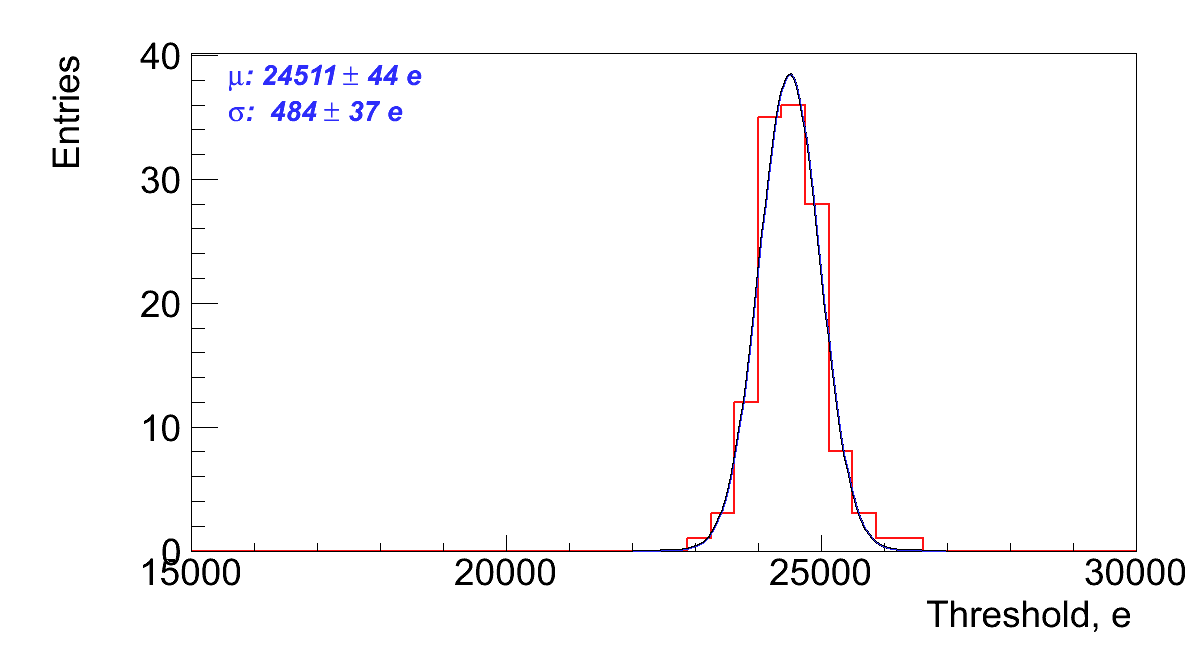
\includegraphics[width=0.8\columnwidth,keepaspectratio]{thrdisp.png}
	\caption{Typical threshold dispersion within a chip.}
	\label{fig:thrdisp}
\end{figure}

Threshold charge must be the same across the channels in a detector, otherwise the track-finding algorithms would be biased by the potential extra hits. Any spread in the response among the different channels of a chip results in a spread of the efficiency and noise occupancy which degrades effective performance. This leads to a requirement that the channel-to-channel variations in threshold and noise are kept to a minimum. Threshold dispersion is defined to be a standard deviation of the distribution of means obtained from the parameters of the complementary error function fit. The noise and threshold dispersion constants for each individual detector channel are measured and the values are used by the zero-suppression algorithms implemented in the core logic of the FSSR2 and by calibration procedures to identify defective channels. A comparison of the noise for 33~cm strips with the threshold spread demonstrates that the threshold spread is negligible compared to the noise and does not affect the efficiency and noise occupancy (see Fig.~\ref{fig:thrdisp}). The threshold dispersion agrees with expectations for the FSSR2 chip for the chosen settings.

SVT calibration data are stored in CLAS12 calibration database. The channel calibration table has columns corresponding to sector, layer, chip ID, mean, channel status (good, noisy, open, dead, or masked), ENC, gain, offset, V$_{t50}$ (threshold at 50$\%$ occupancy), and the threshold. There are 21504 rows in the channel calibration table. The ENC and gain are calculated using a calibration amplitude equal to 100 DAC.
The chip calibration table has columns corresponding to layer, sector, chip ID, ENC (electrons), gain (mV/fC), offset (mV), the threshold at 50$\%$ occupancy (V$_{t50}$, mV), threshold dispersion (electrons), chip gain (low, high), BLR mode (off, on), BCO time (ns), shaper time (ns), 8 ADC thresholds in DAC. There are 168 rows in the chip calibration table. 


\section{Simulation}

%\subsection{Expected physics performance}

%A series MC simulation have been used to calculate the acceptance of the central detector and have reconstructed physics parameters for types of events that are of interest. Fig. ... shows the missing mass resolution expected for MC simulation studies for a number of different reactions. For all cases studied, the results show that it is possible to identify the missing particle for each reaction.
%Figure ... shows the missing mass spectrum expected when pion is detected in the central tracker. There is sufficient resolution to study resonant production and to compare, for example, s, t, and u channel processes.

\subsection{Detector simulation}

A realistic model of the SVT has been developed, describing the location and composition of all modules, with material description based on the engineering drawings and assembly procedures, and confirmed by the survey measurements during integration. The SVT design and module layout were validated by Geant-4-based simulated detector performance studies demonstrating compliance with the technical requirements and engineering models. A 3D view of the simulated geometry of the SVT sensors is shown in Fig.~\ref{fig:svt3dview}. The SVT model is described in the simulation article of this volume. 

\begin{figure}[hbt] 
\centering 
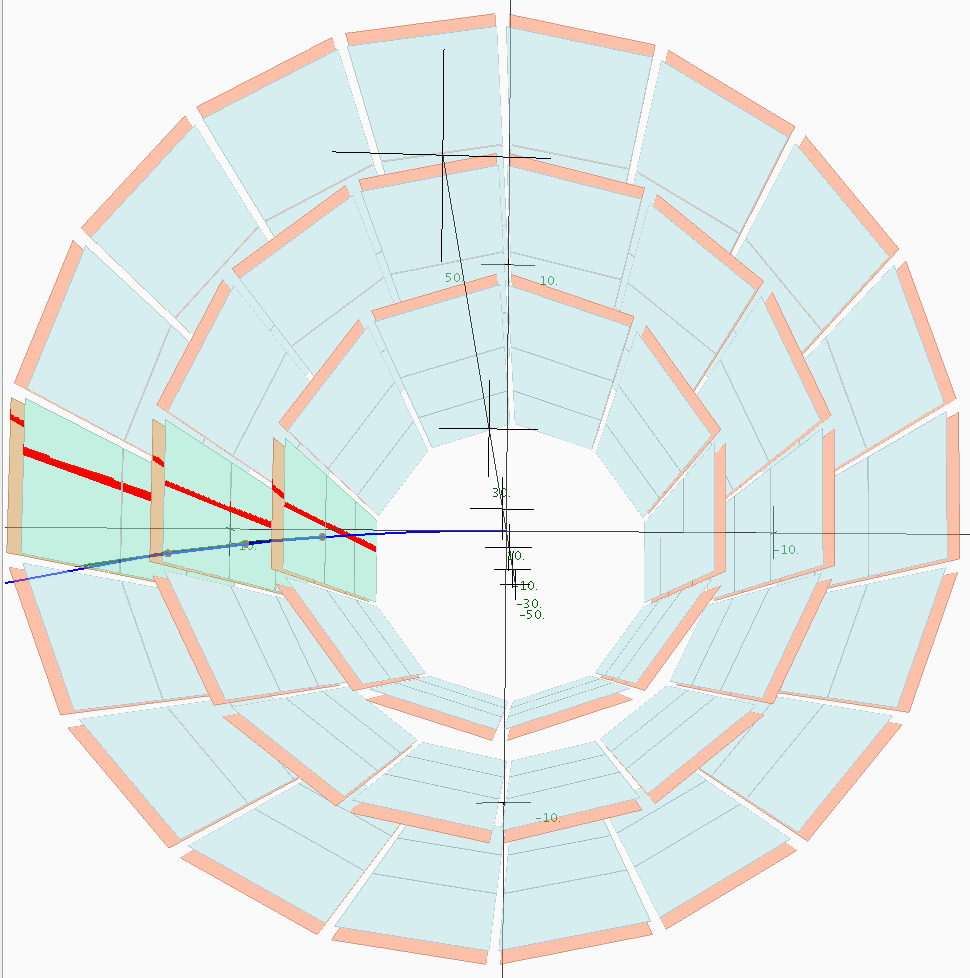
\includegraphics[width=1.0\columnwidth,keepaspectratio]{svt3dview.png}
\caption{3D view of the simulated SVT detector geometry.}
\label{fig:svt3dview}
\end{figure}

According to the results of GEANT simulation of the SVT, a resolution of 50~$\mu$m in the bending plane is needed to measure, with a precision better than 5$\%$, tracks with momentum up to 1~GeV (see Fig.~\ref{fig:PtRes}) \cite{MC1,MC2}. At low momenta the degradation of the resolution is caused by multiple scattering.

\begin{figure}[hbt]
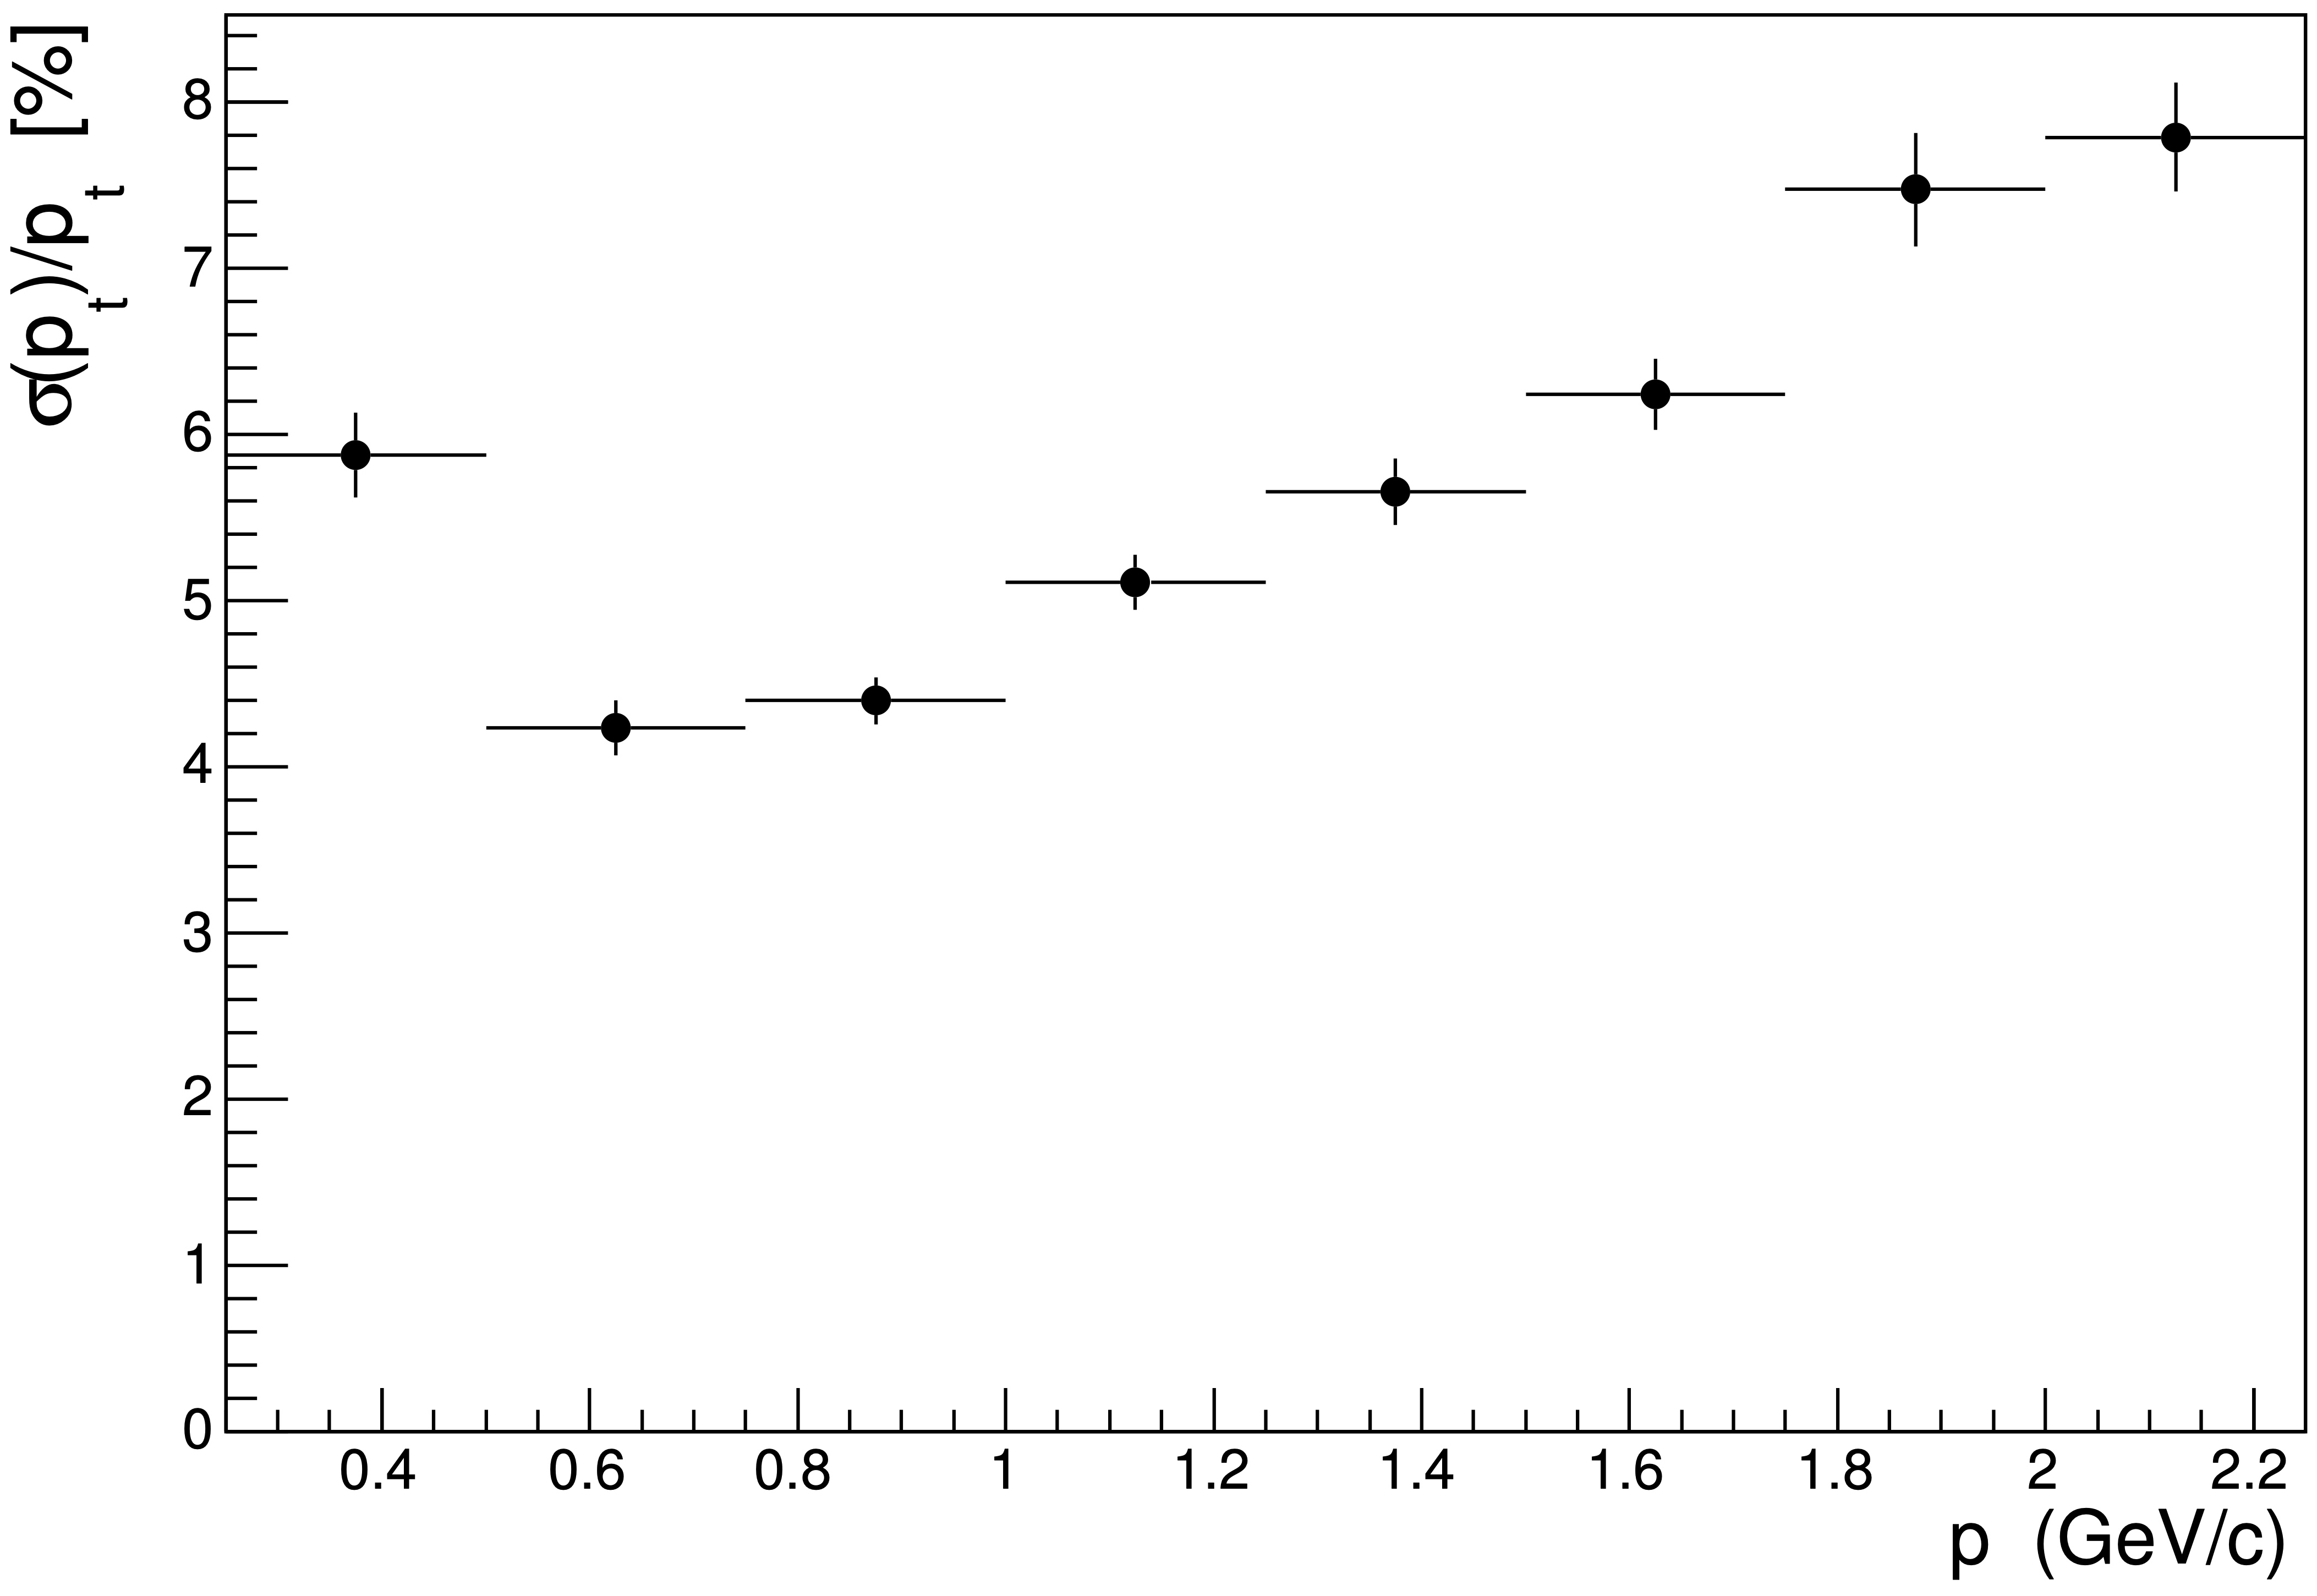
\includegraphics[width=1.0\columnwidth,keepaspectratio]{PtResol.jpg}
\caption{Simulated SVT momentum resolution.}
\label{fig:PtRes}
\end{figure}

Centroid residual distribution for the simulated muon tracks generated in the interval 0.5--2 GeV is shown in Fig.~\ref{fig:centroid-residual-mc}. Cluster centroids were calculated based on the charge weighting method. The spacial resolution of the sensors in the transverse plane using the ideal SVT geometry with no misalignments was found to be about 30~$\mu$m. 

\begin{figure}[hbt]
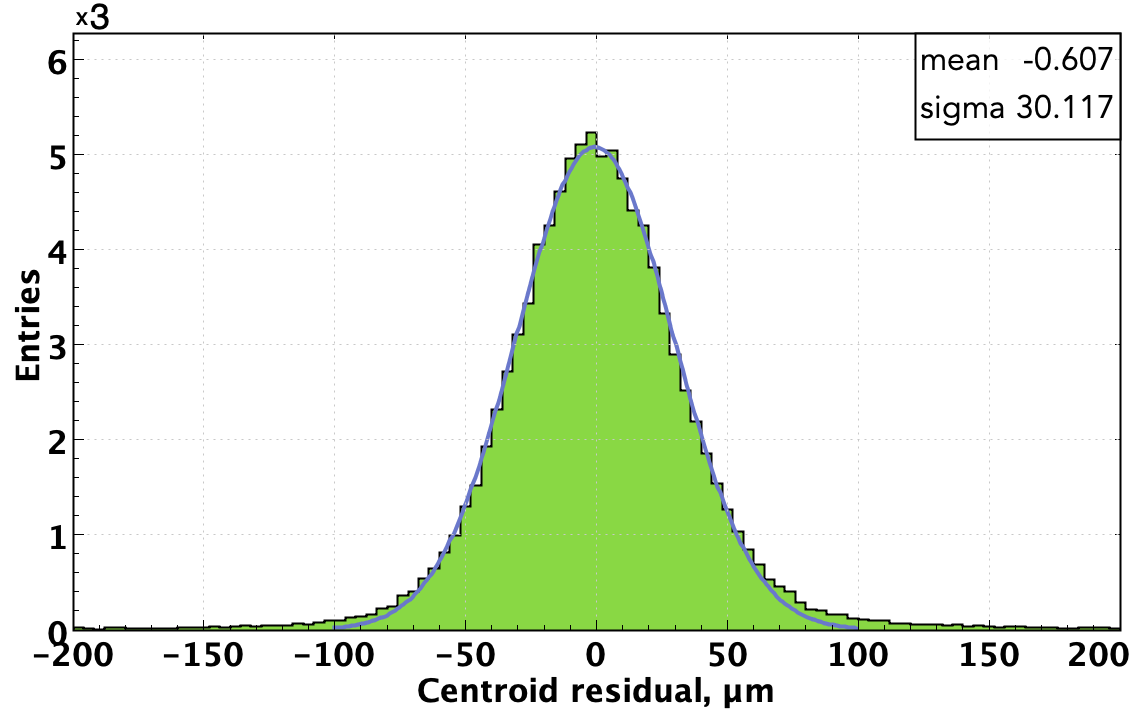
\includegraphics[width=1.0\columnwidth,keepaspectratio]{centroid-residual-mc.png}
\caption{Simulated centroid residual distribution for the SVT module.}
\label{fig:centroid-residual-mc}
\end{figure}

\subsection{Backgrounds, energy deposition, dose rates}

Radiation-induced bulk and surface detector damage studies have been conducted with charged hadrons, leptons, neutrons, and $\gamma$-ray photons. The radiation damage produced by different particles with different energies are scaled under the assumption of the Non-Ionizing Energy Loss (NIEL) hypothesis as the radiation damage in the silicon bulk depends only on the non-ionizing energy loss. The damage caused by different particles is referenced to the damage from 1 MeV neutrons. The standard value for the NIEL of 1 MeV neutrons is 95 MeVmb. 

\begin{figure}[hbt] 
\centering 
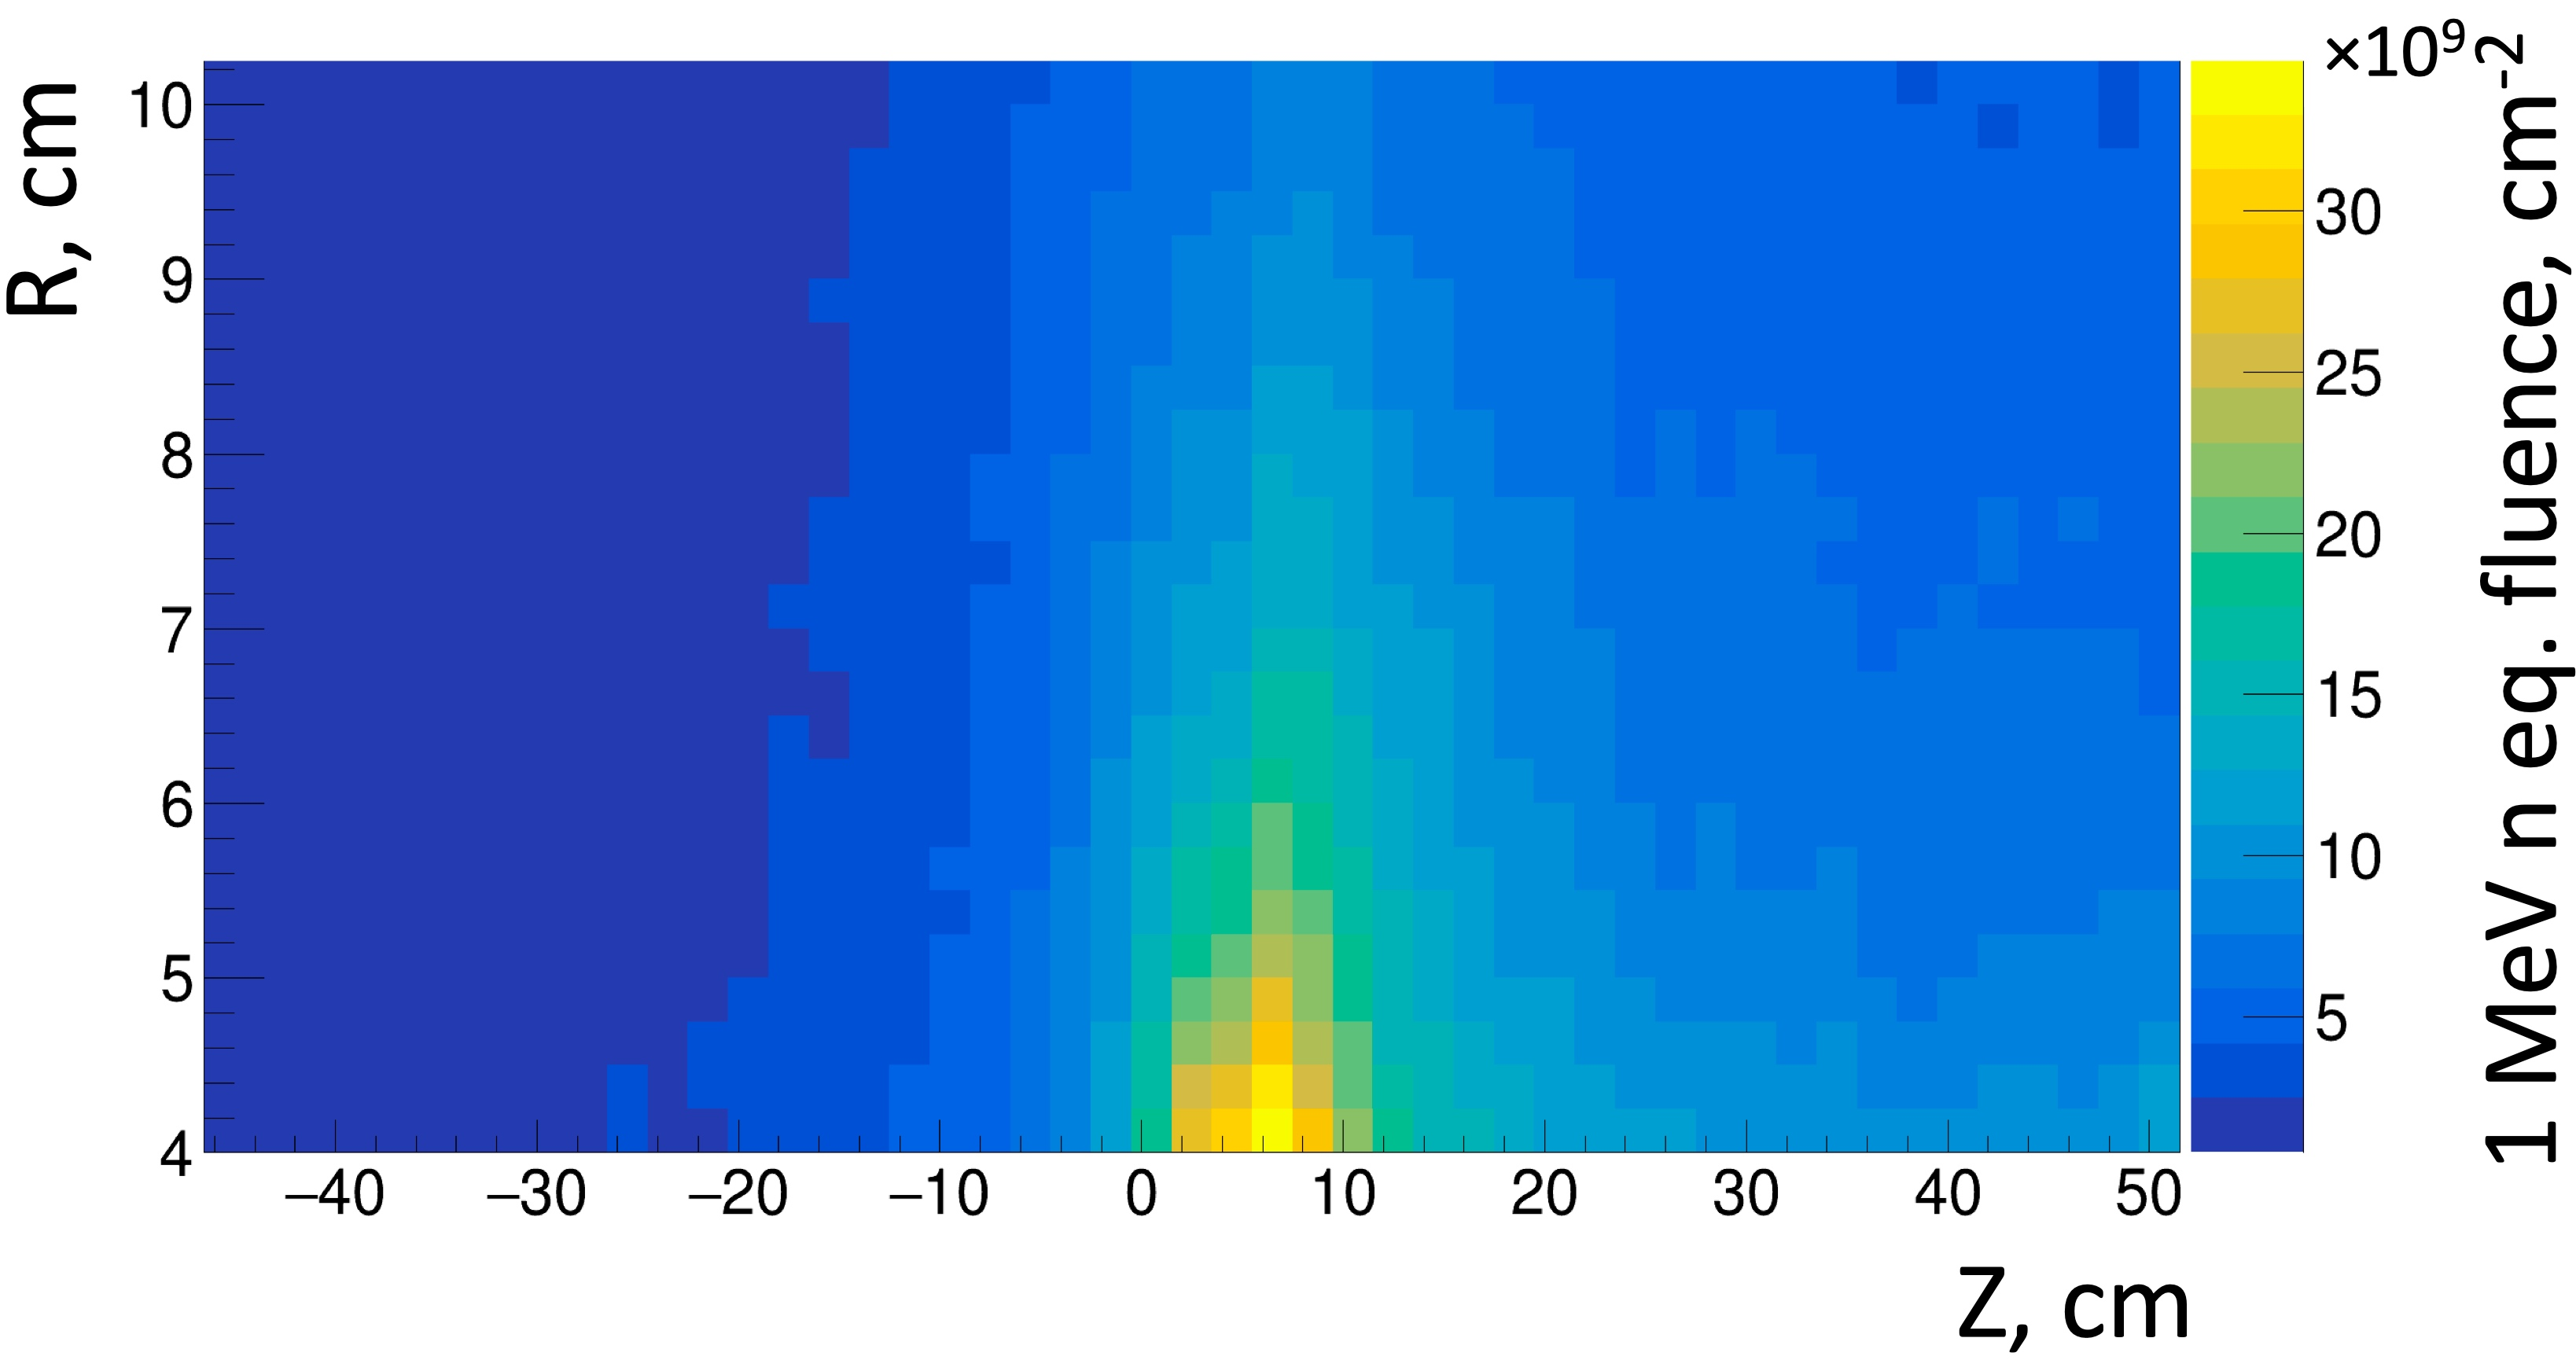
\includegraphics[width=1.0\columnwidth,keepaspectratio]{Pb_1MeVeq.jpg}
\caption{Accumulated 1MeV equivalent neutron fluence for the lead target.}
\label{fig:fluka1}
\end{figure}

To calculate the effects of different target configurations on the SVT detector,  FLUKA~\cite{FLUKA1, FLUKA2} simulations have been performed. In order to include the hadron electro-nuclear production, a dedicated source term has been used to enhance the physics production from the target, since it is a key in radiation estimates for targets with radiation length below 4$\%$. To assess the radiation damage to the SVT, the accumulated 1MeV neutron equivalent fluence has been recorded corresponding to the planned run conditions. For the experiment with lead target, the expected exposure was 240 h at beam current of 38 nA with electron beam energy of 6.6 GeV (Fig.~\ref{fig:fluka1}). For deuterium target, the study has been done for the accumulated charge of 108 mC at 11 GeV (Fig.~\ref{fig:fluka2}). In both scenarios the expected doses should not cause substantial degradation of the silicon sensors.

\begin{figure}[hbt] 
\centering 
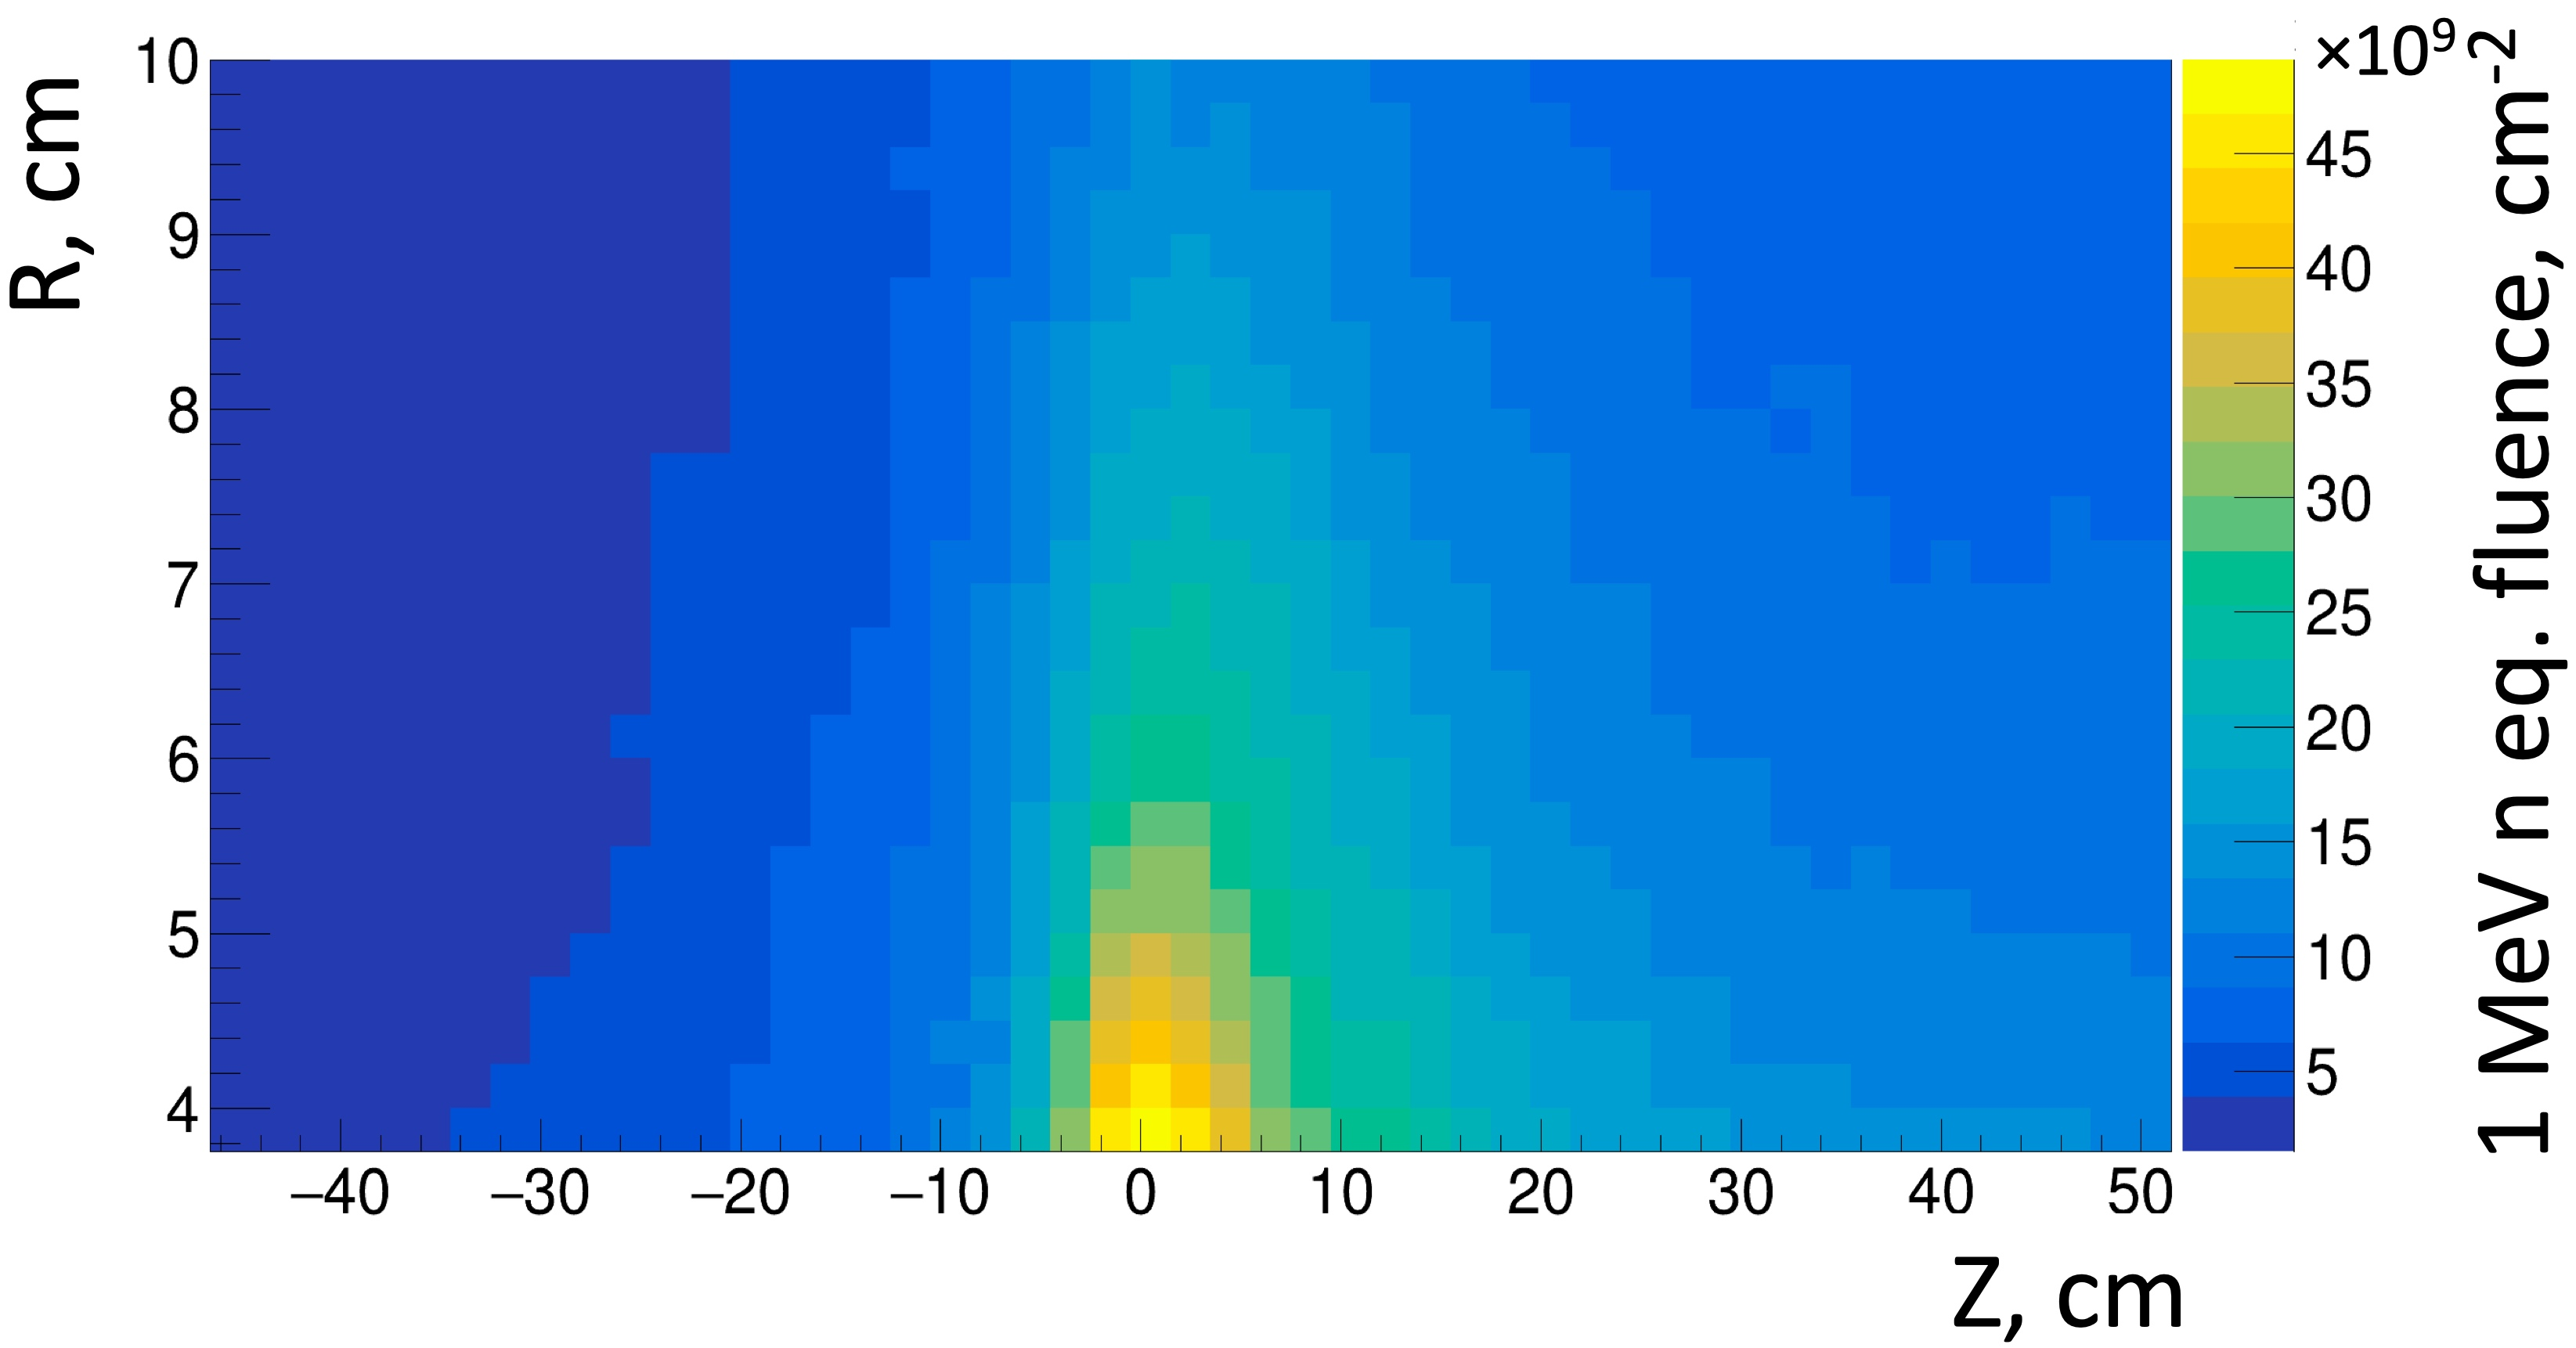
\includegraphics[width=1.0\columnwidth,keepaspectratio]{Deuterium_1MeVeq.jpg}
\caption{Accumulated 1MeV equivalent neutron fluence for the deuterium target.}
\label{fig:fluka2}
\end{figure}

FLUKA simulations of radiation damage levels have been performed in terms of 1MeV equivalent neutron fluence and high energy hadron equivalent fluence which is proportional to the rate of Single Event Effects (SEE)~\cite{FLUKA3}. Estimated levels of radiation damage in radial direction are presented in Fig.~\ref{fig:rad-levels-radial}) for liquid hydrogen and carbon targets at nominal beam currents. Also shown the radiation levels for the tagger magnet yoke during the beam tuning (see the beam line section in this volume).

\begin{figure}[hbt] 
\centering 
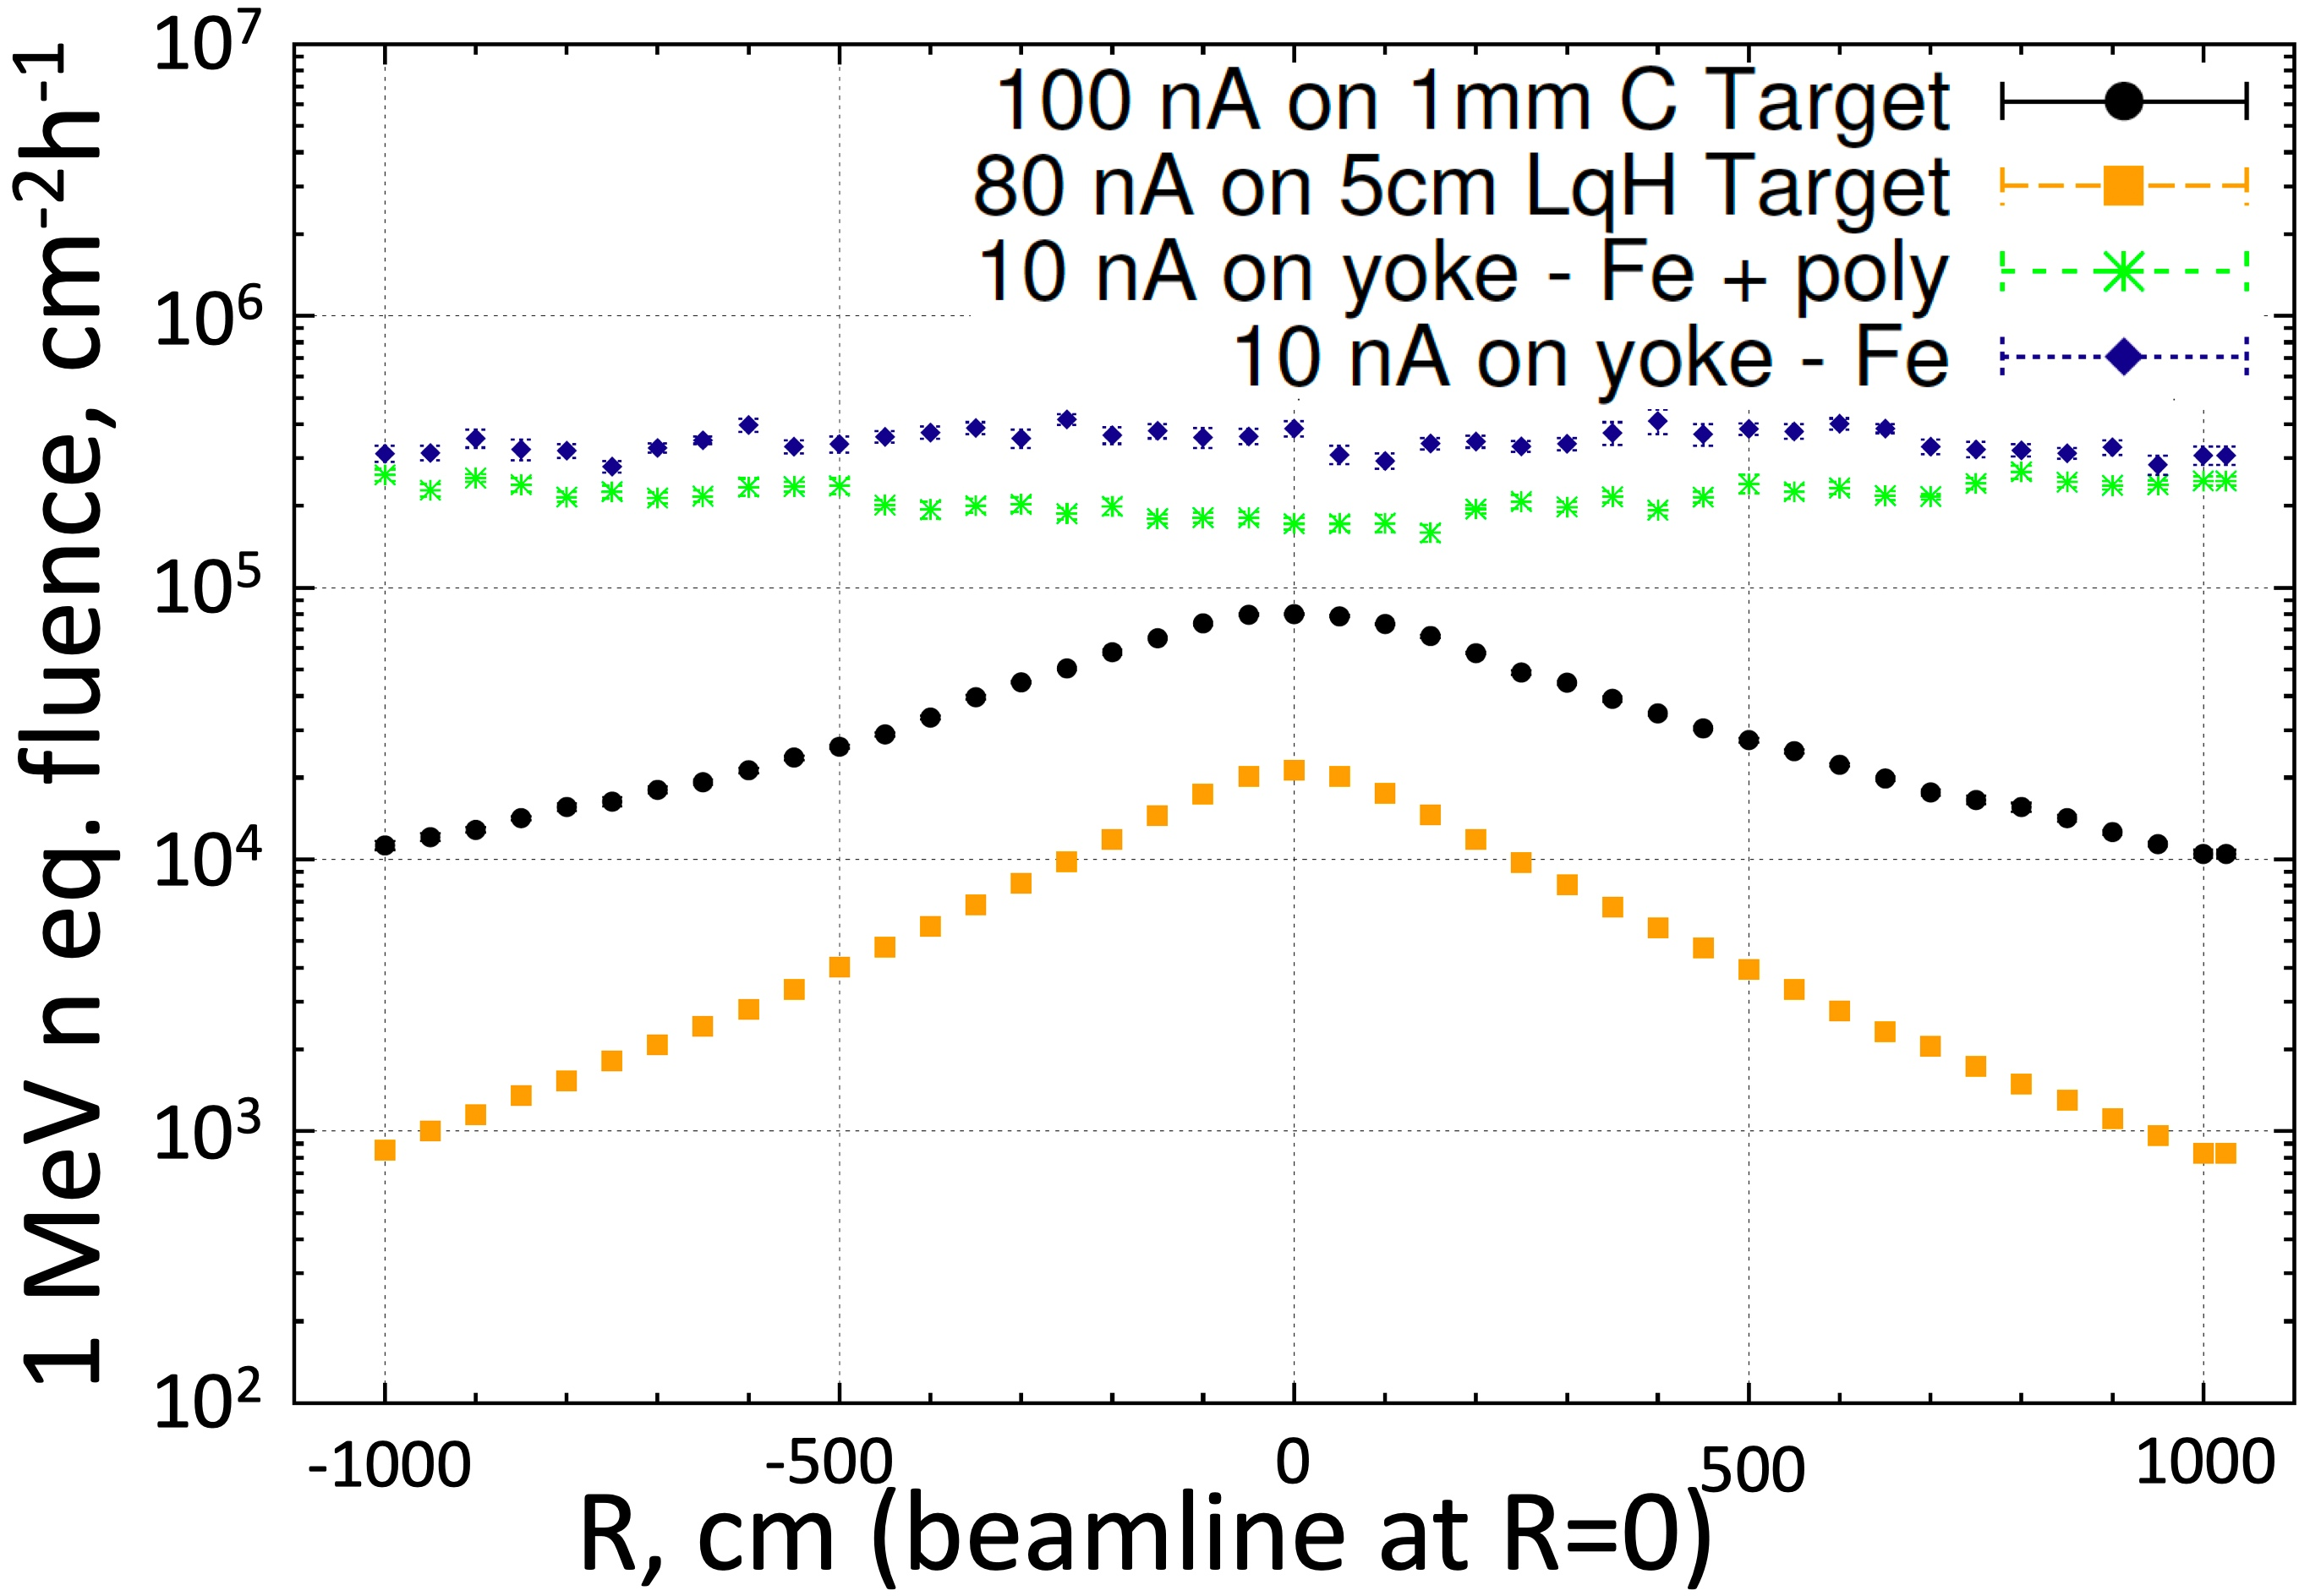
\includegraphics[width=1.0\columnwidth,keepaspectratio]{rad-levels-radial.jpg}
\caption{Estimated levels of radiation damage in radial direction in terms of 1MeV neutron equivalent fluence in silicon.}
\label{fig:rad-levels-radial}
\end{figure}

Simulations of beam-related backgrounds were performed for several thicknesses of a tungsten shielding cylinder around the CLAS12 target covering the first SVT layer. 
 
\begin{figure}[hbt] 
\centering 
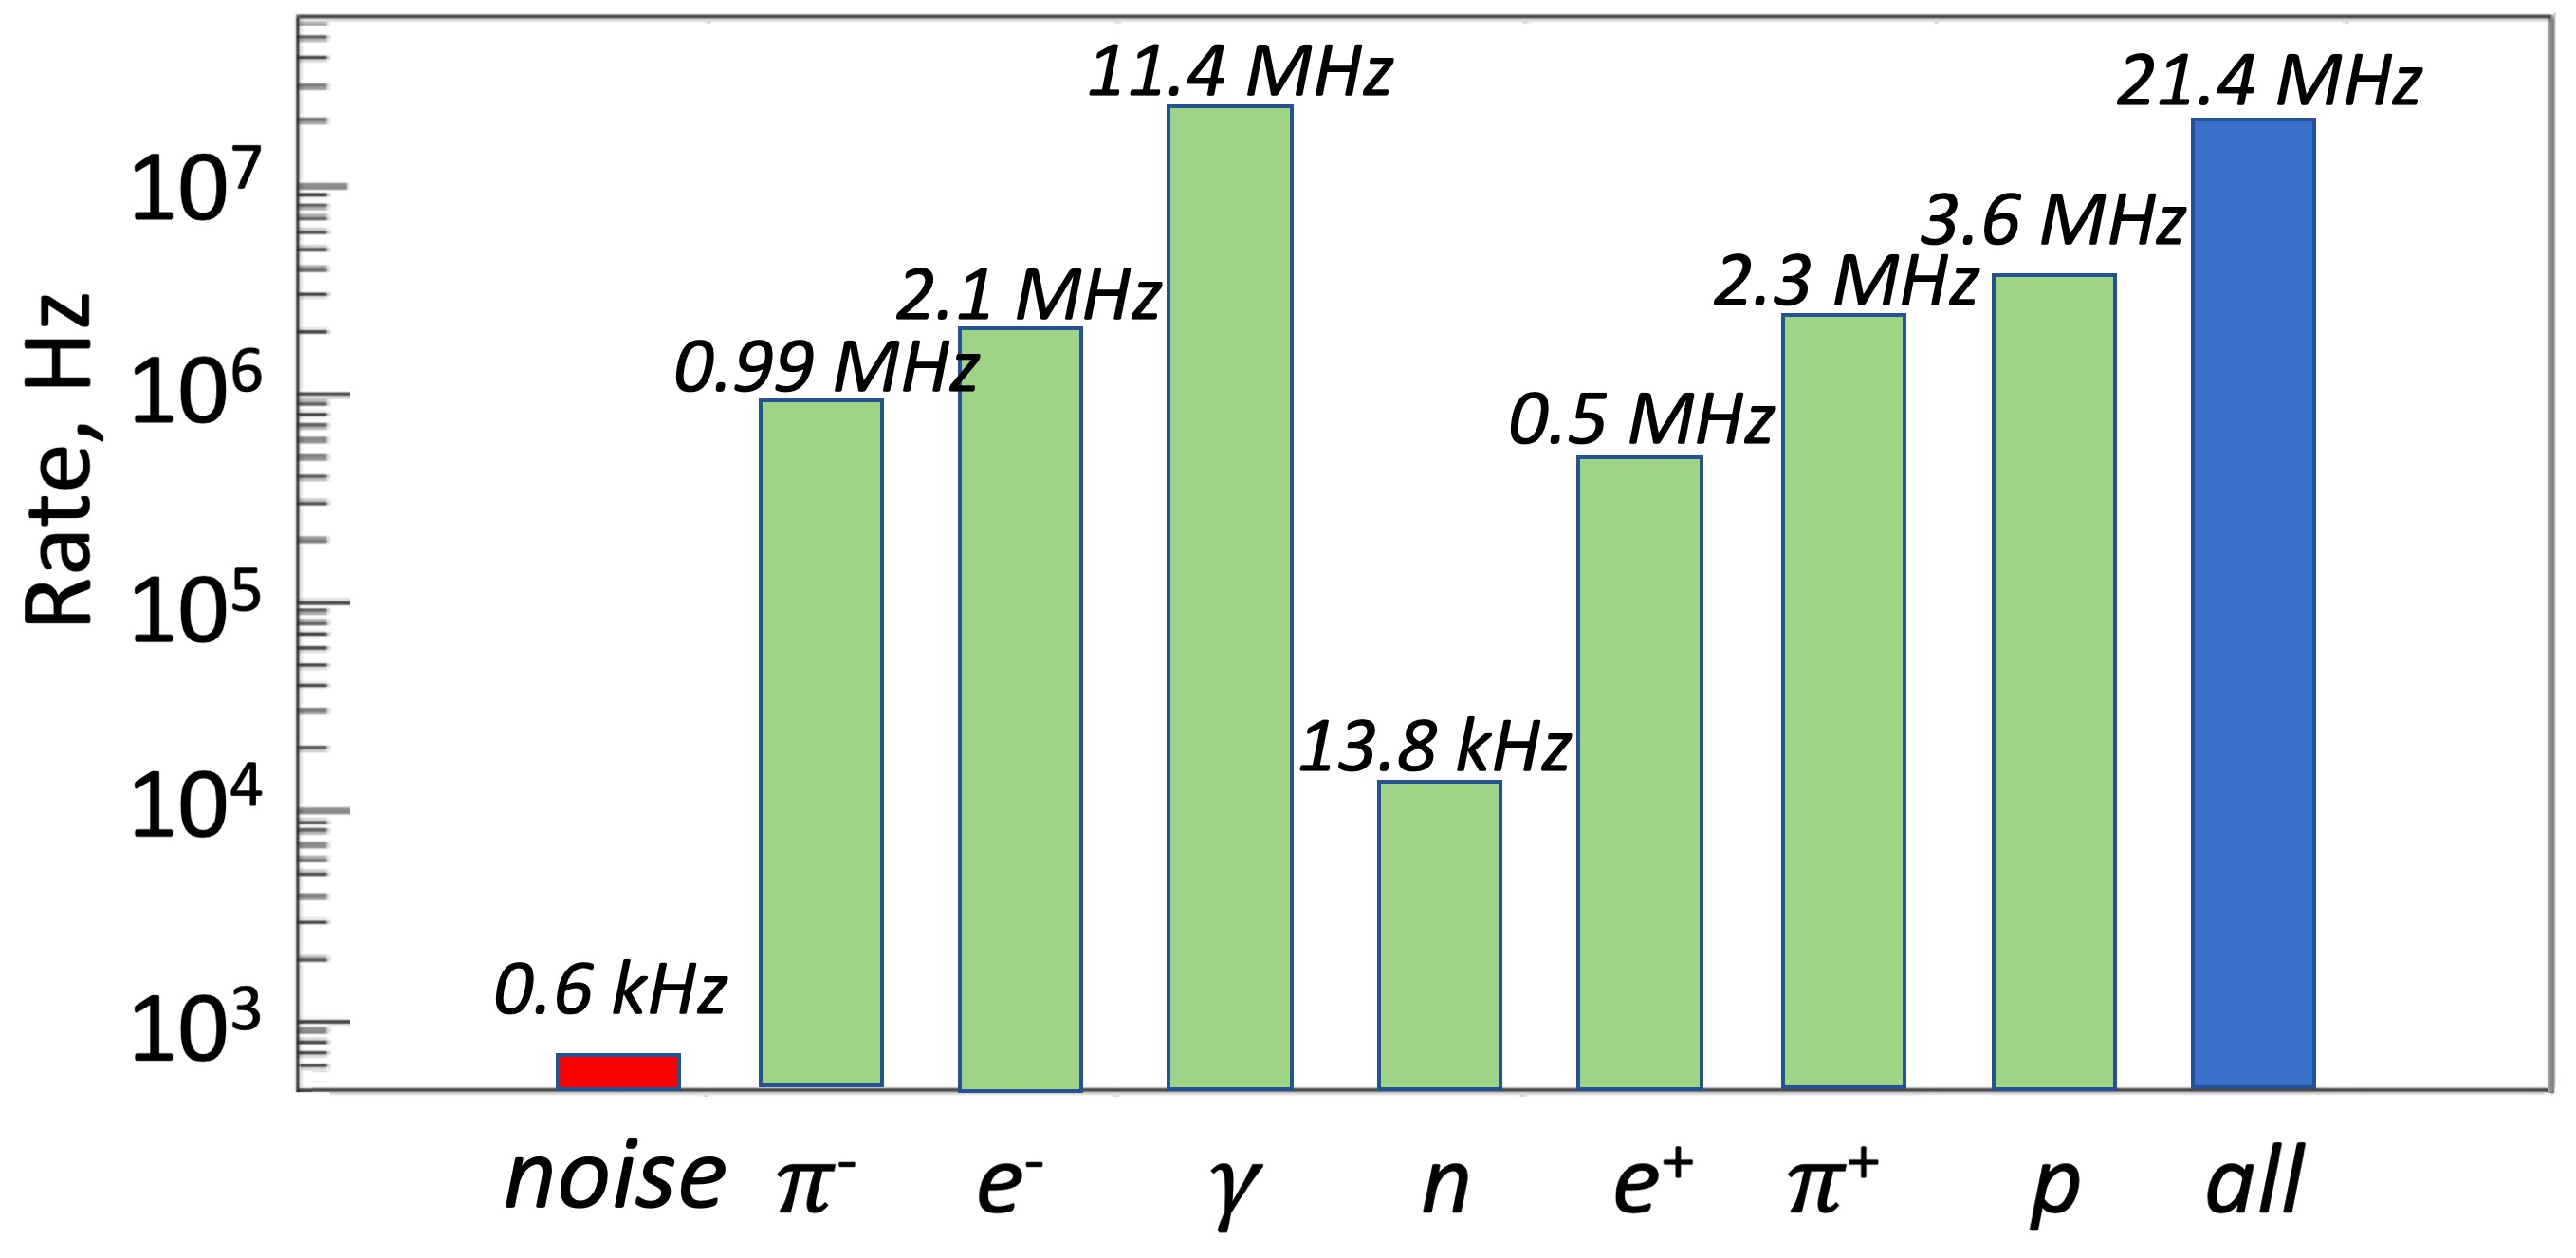
\includegraphics[width=1.0\columnwidth,keepaspectratio]{rates-lh2.jpg}
\caption{Rates in the first SVT layer for a 5-cm long liquid hydrogen target at the nominal CLAS12 operating luminosity of 10$^{35}$cm$^{-2}$s$^{-1}$.}
\label{fig:rates-lh2}
\end{figure}

Fluences, radiation doses, and 1 MeV neutron damage rates in the SVT were calculated for different particles. Rates were estimated for liquid hydrogen, liquid deuterium, carbon, iron, and lead targets. For each event, 124,000 electrons going through the target within a 248.5-ns time window were simulated. This corresponds to the full CLAS12' 10$^{35}$cm$^{-2}$s$^{-1}$ luminosity on a 5-cm-long liquid-hydrogen target at 11 GeV beam energy. Rates in the first SVT layer for a liquid-hydrogen target are shown in Fig.~\ref{fig:rates-lh2}. For carbon target at a threshold of 40 keV the hadronic rate was estimated to be 5 MHz (total rate 40 MHz) with strip hit rates of 3.1 kHz (region 1), 2.2 kHz (region 2), and 1.7 kHz (region 3). The energy deposited in layer 1 for the electromagnetic and the hadronic particles is shown in Fig.~\ref{fig:energy-deposited-l1}. At a threshold of 30 keV, 92$\%$ of the electromagnetic background is rejected while preserving  99.5$\%$ of the signals coming from the hadrons~\cite{TDRSVT}.

\begin{figure}[hbt] 
\centering 
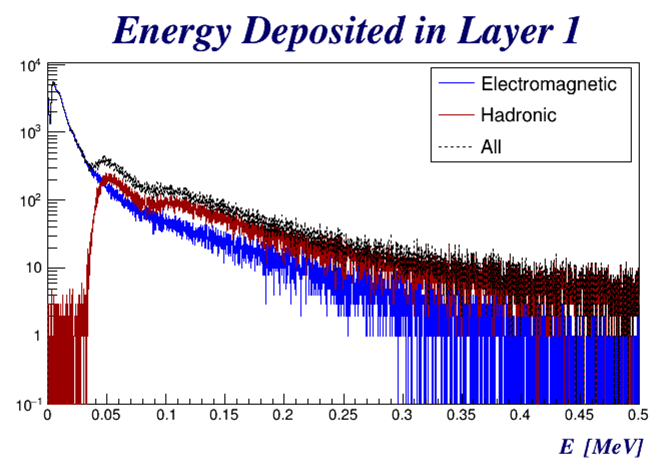
\includegraphics[width=1.0\columnwidth,keepaspectratio]{energy-deposited-l1.png}
\caption{Energy deposited in the SVT layer 1 for electromagnetic and hadronic particles for a liquid hydrogen target at the nominal CLAS12 operating luminosity.}
\label{fig:energy-deposited-l1}
\end{figure}

A tungsten shield 51~$\mu$m thick is installed on the target scattering chamber. The shield consists of 2 sheets mounted over the top and bottom halves of the foam cylinder referenced to the SVT common ground. The SVT rates and radiation damage benefit from the inclusion of the tungsten shield. The rates have been compared with physics run data at several beam currents.

While the gamma fluences / doses show a dramatic decrease with the introduction of shielding, the total fluences and doses decrease significantly for the thinner configuration and do not vary much for thicker tungsten (see Fig.~\ref{fig:rates-l1}). The photon radiation dose becomes negligible for 50 $\mu$m or more of tungsten with total 1 MeV equivalent radiation dose about 65 krad per year on a liquid-hydrogen target. For 15 years of running the experiment on a carbon target the estimated radiation dose for the sensors is 2.5~Mrad (with 50 $\%$ operation) \cite{TDRSVT}. 

\begin{figure}[hbt] 
\centering 
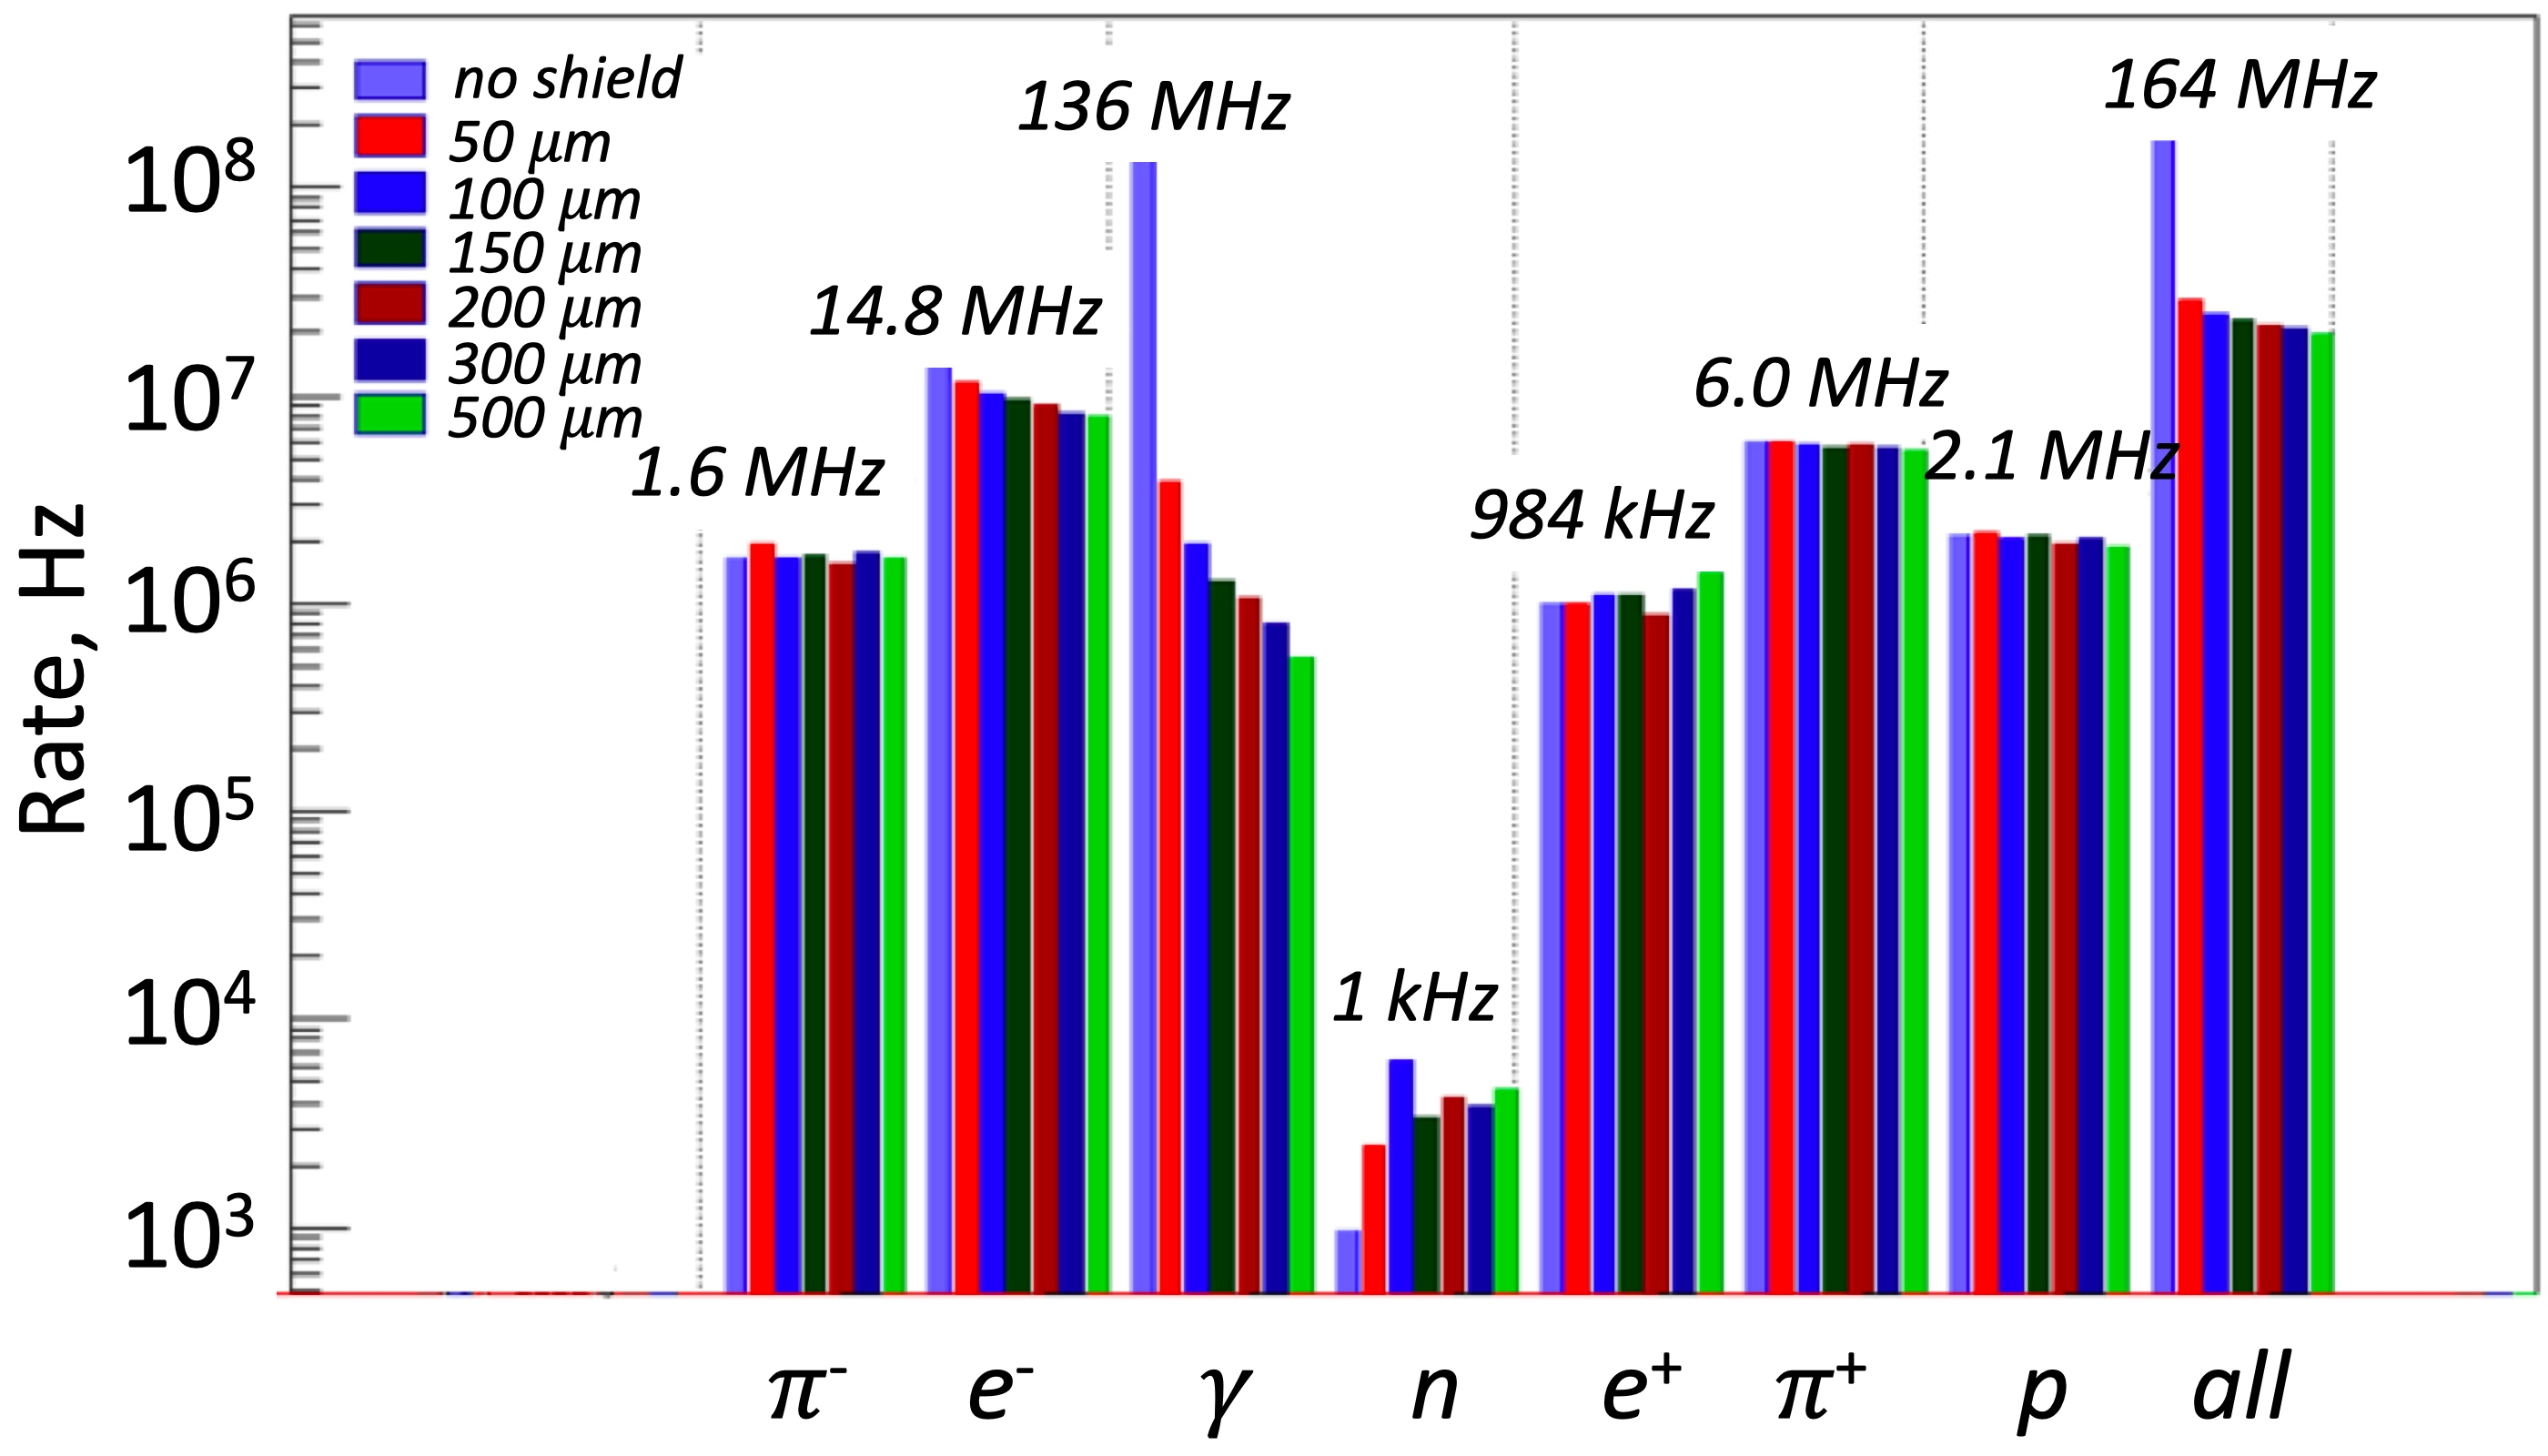
\includegraphics[width=1.0\columnwidth,keepaspectratio]{rates-l1.jpg}
\caption{Rates in the first SVT layer for different tungsten shield thickness from 50 to 500 $\mu$m for a liquid hydrogen target at the nominal CLAS12 operating luminosity. No energy threshold cut applied.}
\label{fig:rates-l1}
\end{figure}

An estimate of the double hit rate was performed. Fig.~\ref{fig:double-hit-rate} shows the probability of the double hits in the inner region of the SVT. The ratio of the double hits to the single hits was found to be about 1$\%$.

\begin{figure}[hbt] 
\centering 
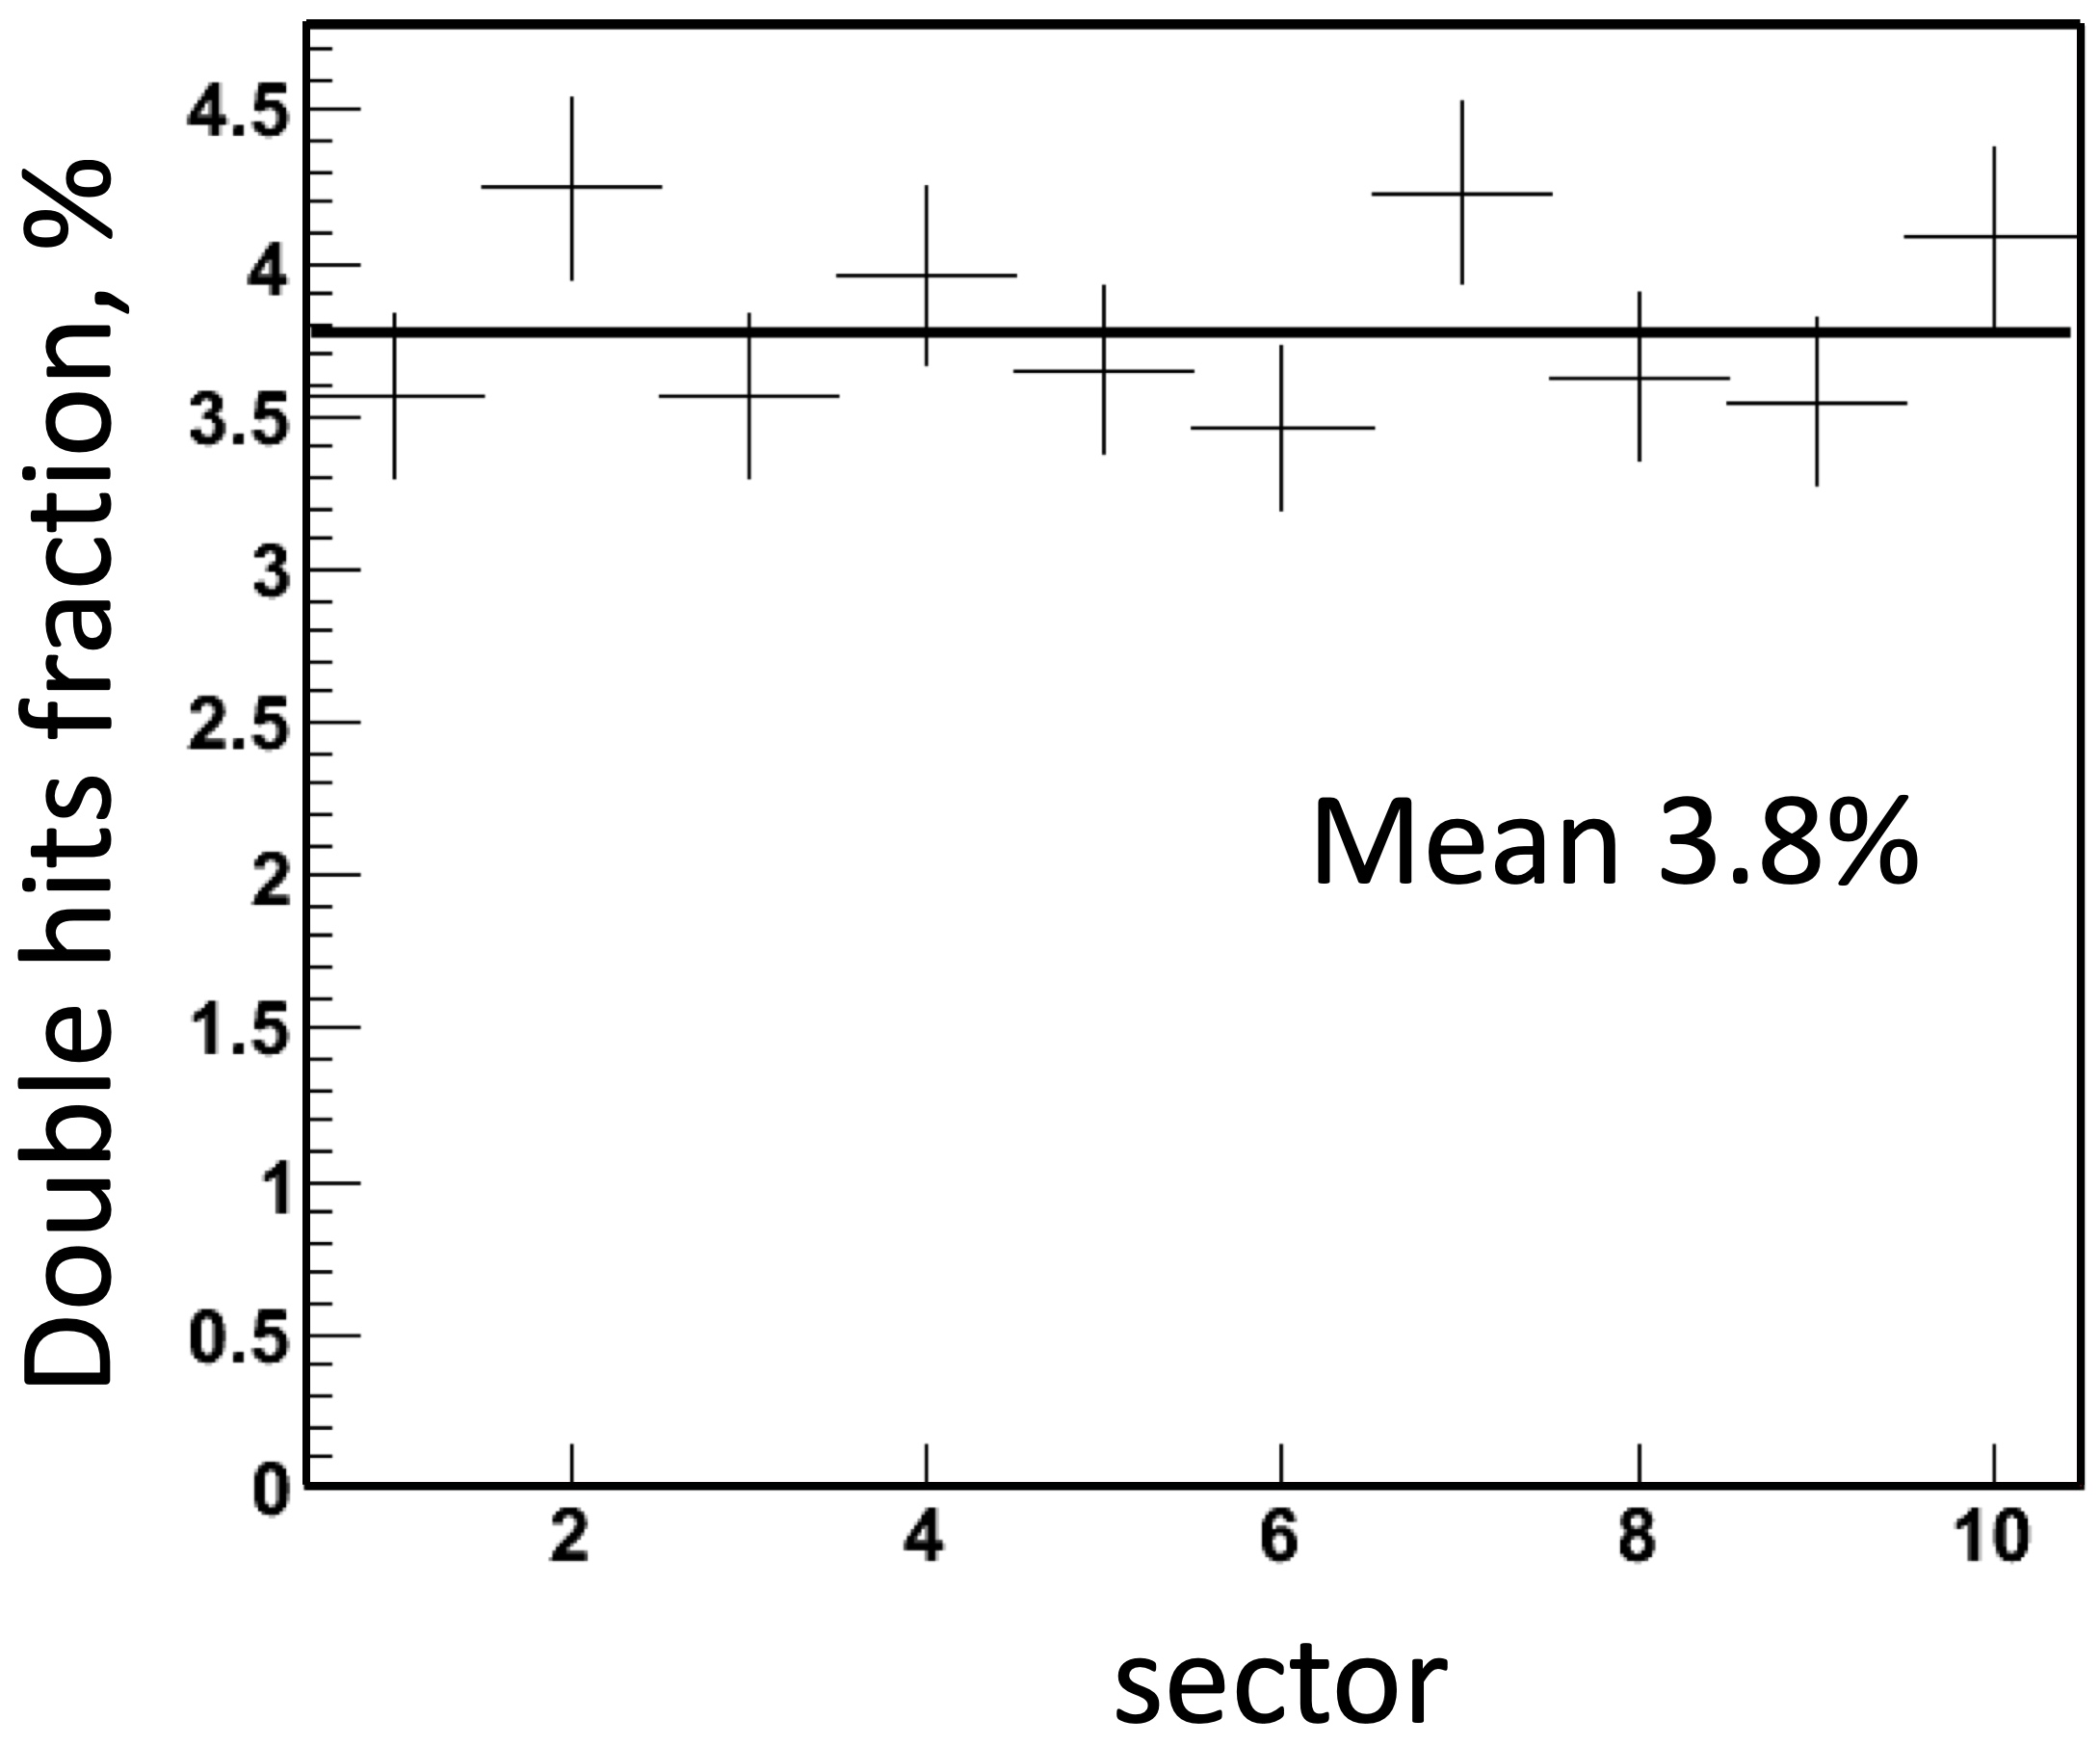
\includegraphics[width=1.0\columnwidth,keepaspectratio]{double-hit-rate.jpg}
\caption{Double hit fraction in the region 1 with liquid hydrogen target.}
\label{fig:double-hit-rate}
\end{figure}

\subsection{Magnetic Field}

Due to the constrains on the maximum length of the cables, the readout, slow controls, and power supply crates are installed on a movable service cart within few meters from the detector. To assess the potential impact of the solenoid field on the SVT DAQ, a magnetic field map was simulated for the location of the power supply and readout crates. Fig.~\ref{fig:solenoid-field}) shows that the maximum strength of the field for the crates is at an acceptable level of 100 G.

\begin{figure}[hbt] 
\centering 
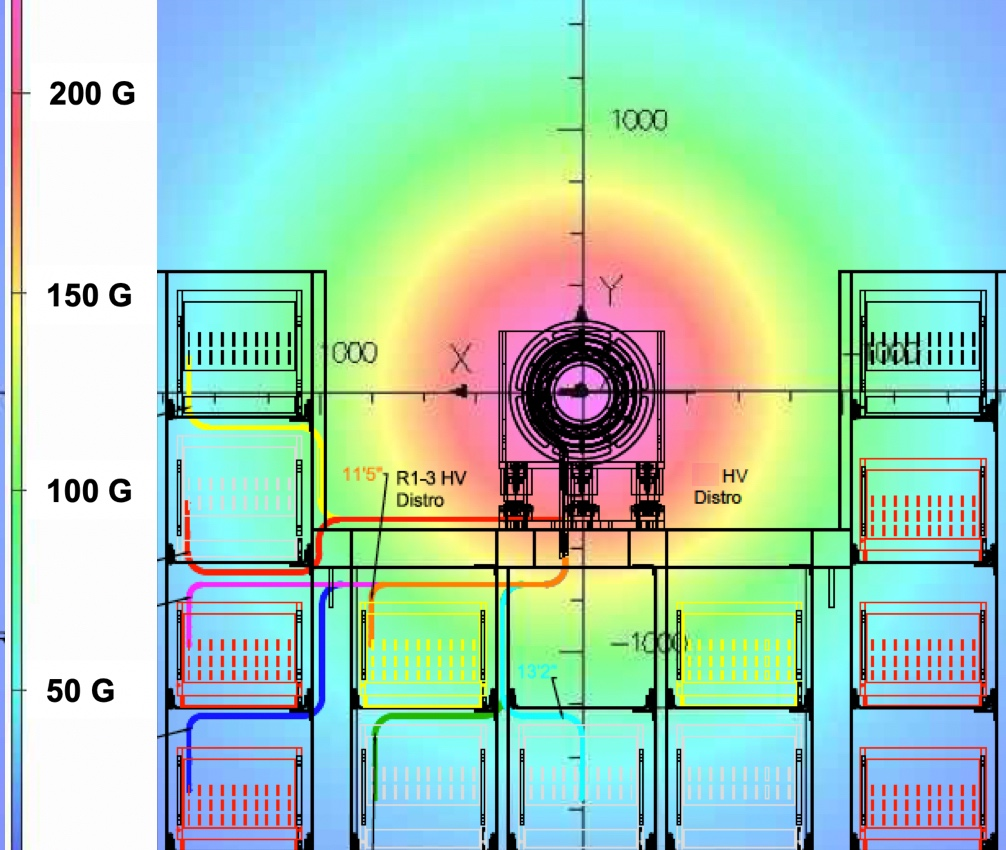
\includegraphics[width=1.0\columnwidth,keepaspectratio]{solenoid-field.jpg}
\caption{Solenoid field map at the location of the SVT service cart.}
\label{fig:solenoid-field}
\end{figure}




\section{Performance}The HTCC is one of the major CLAS12 systems used in experiments with the electron beam. The most important aspects of the HTCC performance are that it provides good timing, high electron detection efficiency, high signal strength, and high rejection factor of charged pions. All these parameters are critical for the quality of the data obtained in experiments since the detector, in combination with the forward calorimeter [ref. to ECAL], provides a fast trigger signal for CLAS12. As shown in section 6 the MC prediction for the HTCC for electrons is $\approx$100\%. Fig.~\ref{fig:RAFO_2GeV}. shows the experimentally measured electron detection efficiency for elastically scattered electrons at 2 GeV. The corresponding thresholds applied were approximately 2.5 photoelectrons. Measurements were performed using a special procedure with a random trigger that was not correlated with the HTCC. There were observed 27 events not detected by the HTCC due to the applied threshold. As shown, the electron detection efficiency is $\eta$ = (99$\pm$0.2)\%, which is in good agreement with the MC estimate. This result can be considered as a conservative estimate due to relatively high threshold used in measurements. Moreover, electrons travel a longer distance in the radiator gas (10 \% to 30 \% difference depending on a scattering angle). For these electrons the signal strength is higher, and therefore the detection efficiency is higher also as compared with the aforementioned efficiency for the elastically scattered electrons.   

\begin{figure}[!ht]
    \centering
    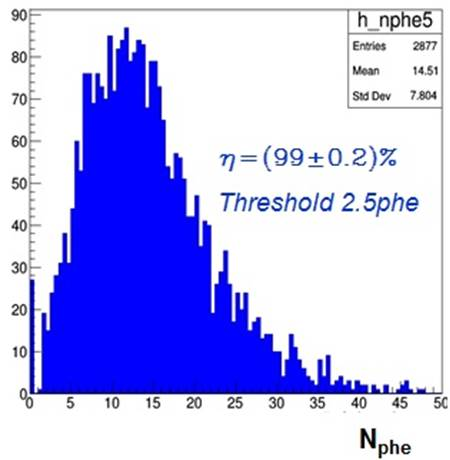
\includegraphics[width=1.0\linewidth,trim={0.0cm 0.0cm 0.0cm 0.0cm},clip]{images/RAFO_2GeV.jpg}
    \caption{Electron detection efficiency for elastically scattered electrons at 2 GeV. Data are obtained with the random trigger not correlated with the HTCC or other detector components of CLAS12.}
    \label{fig:RAFO_2GeV}
\end{figure}

Fig.~\ref{fig:positivePNPEC6595} shows the response of the detector in a wide range of particle momentum. The increase of number of events at high momenta is due to registration of charged pions (above threshold of their registration in the HTCC) and this is clearly illustrated.

\begin{figure}[!ht]
    \centering
    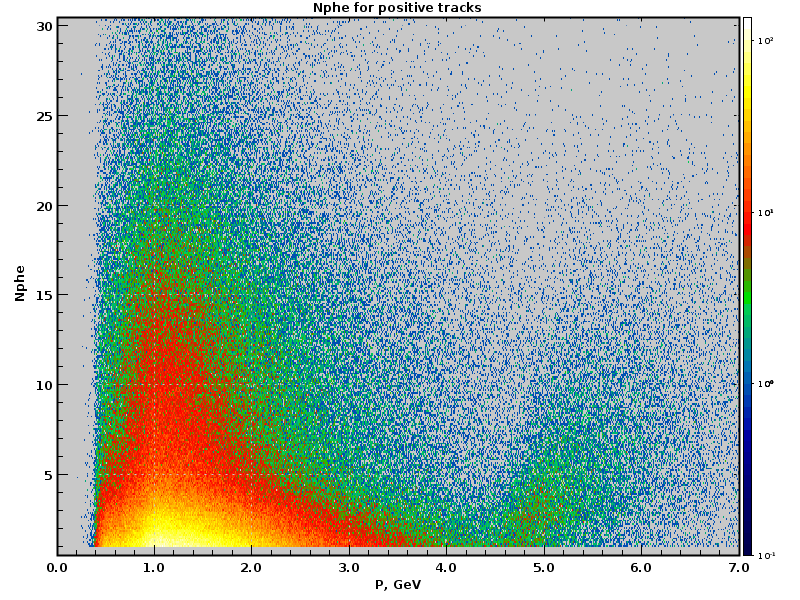
\includegraphics[width=1.0\linewidth,trim={0.0cm 0.0cm 0.0cm 0.0cm},clip]{images/positivePNPEC6595.png}
    \caption{Distributions of the HTCC response in a wide momentum range, including the region beyond the threshold of charged pion registration. Data obtained for positrons and $\pi^{+}$-mesons.}
    \label{fig:positivePNPEC6595}
\end{figure}

\begin{comment}
As shown bellow in the Fig.~\ref{fig:avgNPE_Theta_Phi_Dev_Build-2_NO_HOLES} the signal strength goes up for the utmost mirrors (large electron scattering angles). This is because electrons travel a longer distance in the radiator gas (10\% to 30\% difference depending on angle.) In other words the electron detection efficiency obtained for elastically scattered electrons at 2 GeV can be considered as as a conservative estimate for the efficiency of electron detection at larger angles.
\end{comment} 

The signal strength in the HTCC depends on the actual properties of the mirror facets, such as their final shape and reflectance. The accuracy of the combined mirror assembly and the alignment of the HTCC components (mirror, PMTs, Winston Cones), and the composition of the radiator gas all influence the final results. The FADC histogram of  the typical signal strength distribution obtained in one half-sector \#1 and \#2 of Sector 1 is shown in Fig.~\ref{fig:Signal_S1_HS1_HS2_R1_R2}. The signal strength for scattered electrons averaged over all HTCC channels is shown in Fig.~\ref{fig:Average_HTCC_Signal}. The experimentally measured mean value of 16.3 phe is close to Monte-Carlo simulation results, (see Fig.~\ref{fig:10cm_Targ_5T_Field_Phi}).

\begin{figure}[!ht]
    \centering
    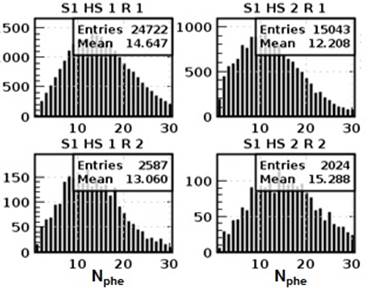
\includegraphics[width=1.0\linewidth,trim={0.0cm 0.0cm 0.0cm 0.0cm},clip]{images/Signal_S1_HS1_HS2_R1_R2.jpg}
    \caption{Typical distributions of the signal strength in channels covering polar angles in the range of $5^\circ$ to $12.5^\circ$ (Ring 1) and $12.5^\circ$ to $20.0^\circ$ (Ring 2) within azimuthal interval of $60^\circ$.}
    \label{fig:Signal_S1_HS1_HS2_R1_R2}
\end{figure}

\begin{figure}[!ht]
    \centering
    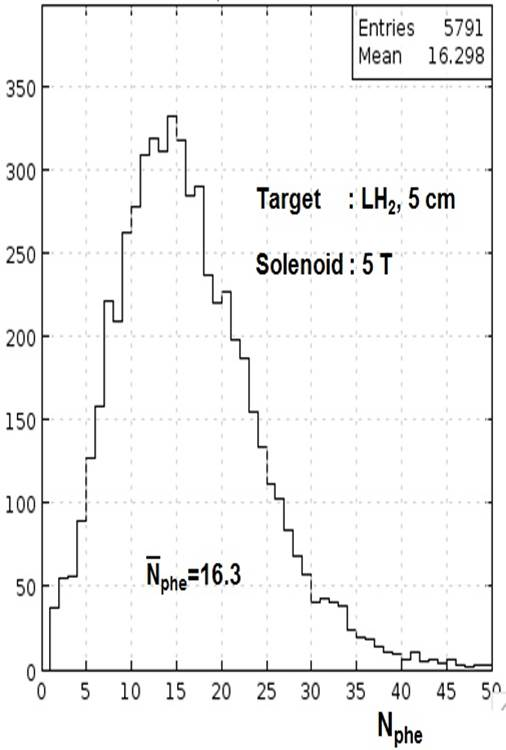
\includegraphics[width=1.0\linewidth,trim={0.0cm 0.0cm 0.0cm 0.0cm},clip]{images/Average_HTCC_Signal.jpg}
    \caption{The HTCC average signal strength for electrons from beam data.}
    \label{fig:Average_HTCC_Signal}
\end{figure}

Fig.~\ref{fig:HTCC_Response_run4013} shows the HTCC response for different electron momenta. Fig.~\ref{fig:avgNPE_Theta_Phi_Dev_Build-2_NO_HOLES}  shows the distribution of the HTCC response over the entire face of the mirror in the $x-y$-plane. Similar distribution is shown in Fig.~\ref{fig:avgNPE_XY_Dev_Build_02npe} obtained at the lower electron detection threshold of 0.2 photoelectrons. At the large electron scattering angles in range of 27.5$^\circ$ to 35$^\circ$, the statistics is lower. Fig.~\ref{fig:statistics_Theta_Phi_Dev_Build_NO_HOLES} shows the distribution of statistics in all 6 sectors. The data shows that the integrated signal strength is about 16.5 photoelectrons.

\begin{figure}[!ht]
    \centering
    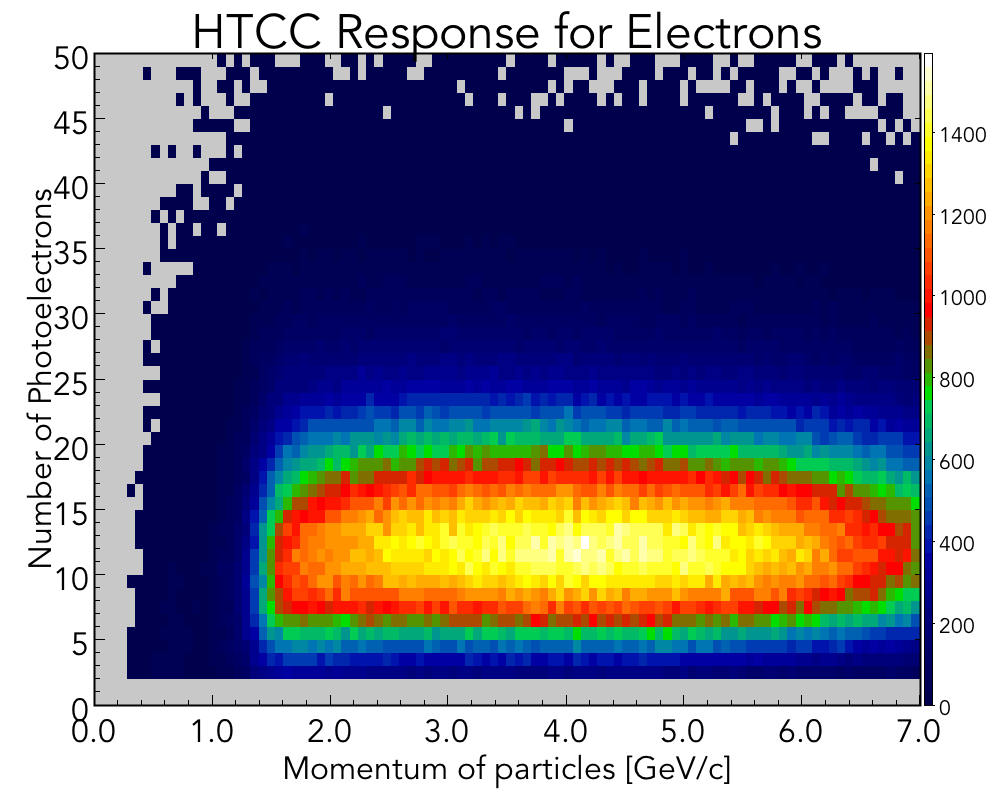
\includegraphics[width=1.0\linewidth,trim={0.0cm 0.0cm 0.0cm 1.73cm},clip]{images/HTCC_Response_run4013.png}
    \caption{The HTCC response for electrons: signal strength vs. momentum at 10.6 GeV energy.}
    \label{fig:HTCC_Response_run4013}
\end{figure}

\begin{figure}[!ht]
    \centering
    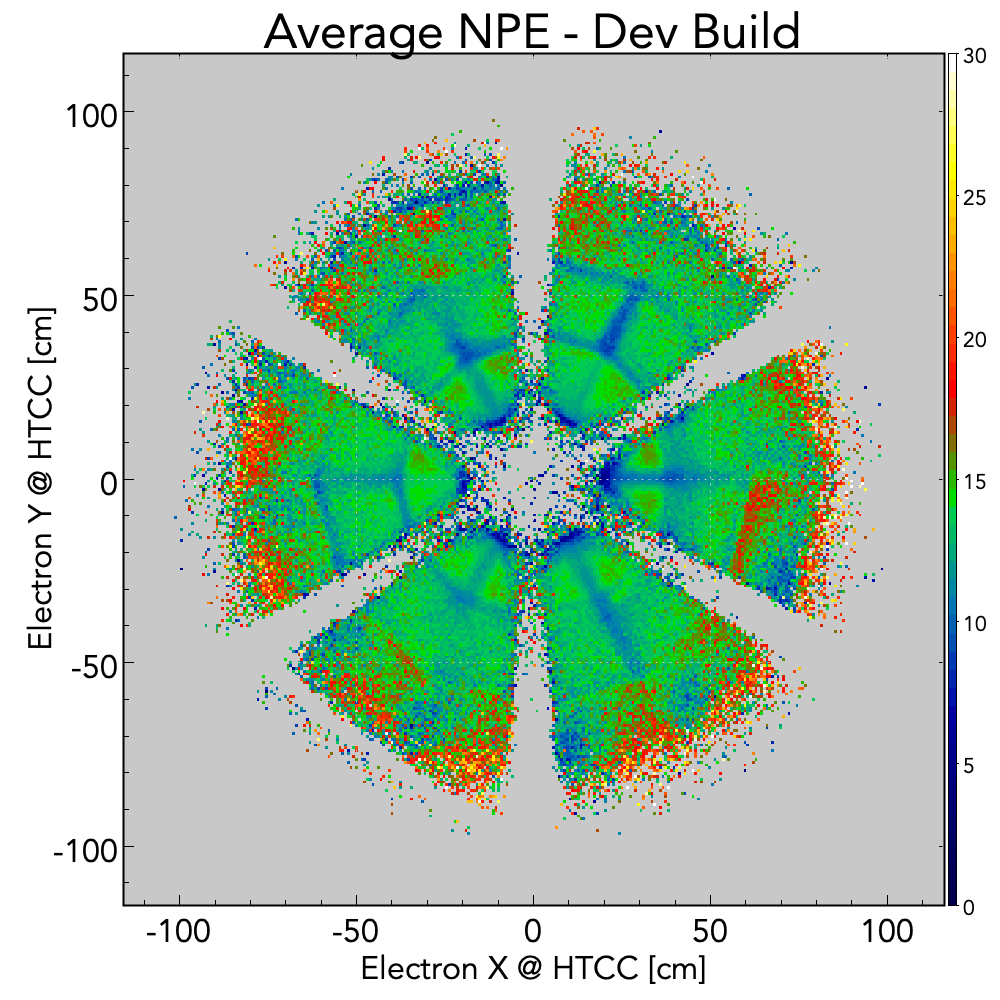
\includegraphics[width=1.0\linewidth,trim={0.0cm 0.0cm 0.0cm 1.67cm},clip]{images/avgNPE_Theta_Phi_Dev_Build-2_NO_HOLES.png}
    \caption{The HTCC response (in $N_{phe}$) for electrons in $x-y$-plane of the mirror.}
    \label{fig:avgNPE_Theta_Phi_Dev_Build-2_NO_HOLES}
\end{figure}

\begin{figure}[!ht]
    \centering
    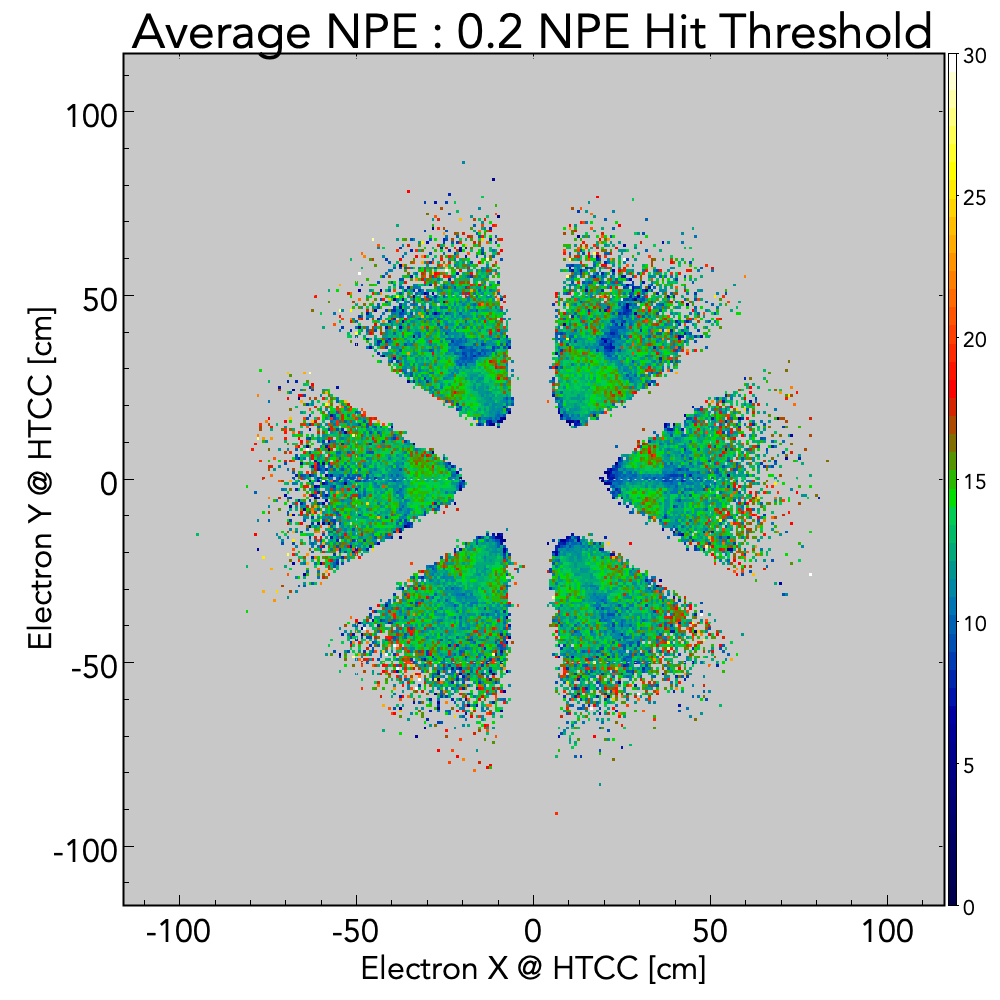
\includegraphics[width=1.0\linewidth,trim={0.0cm 0.0cm 0.0cm 1.67cm},clip]{images/avgNPE_XY_Dev_Build_02npe.png}
    \caption{The HTCC response (in $N_{phe}$) for electrons in $x-y$-plane of the mirror at the electron detection threshold of 0.2 photoelectrons.}
    \label{fig:avgNPE_XY_Dev_Build_02npe}
\end{figure}

\begin{figure}[!ht]
    \centering
    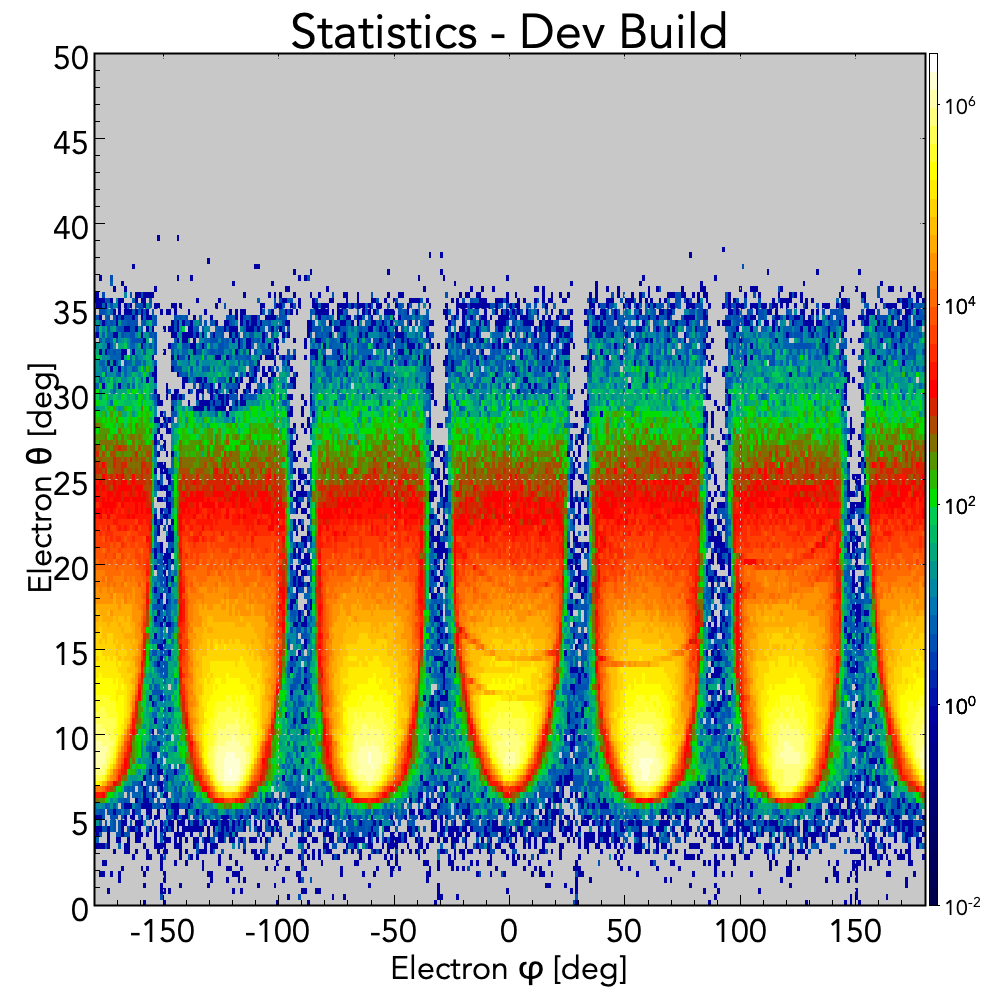
\includegraphics[width=1.0\linewidth,trim={0.0cm 0.0cm 0.0cm 1.67cm},clip]{images/statistics_Theta_Phi_Dev_Build_NO_HOLES.png}
    \caption{Distribution of statistics in all 6 sectors.}
    \label{fig:statistics_Theta_Phi_Dev_Build_NO_HOLES}
\end{figure}

We also note that in cases when the electrons cross the mirror close to its edges (at approximately at 5$^\circ$ and 35$^\circ$) one should expect unavoidable losses in the signal strength: some part of the Cherenkov light just passes by the mirror. As far as the internal borders between adjacent mirrors are concerned, there are similar losses that take place and are finally partially compensated due to the complete azimuthal symmetry of the detector, see Fig.~\ref{fig:avgNPE_Theta_Phi_Dev_Build-2_NO_HOLES}. The width of that area along internal boundaries that is deformed in the direction normal to the mirror face due to the shrinkage of the glue is estimated between $\sim$5 to $\sim$10 mm. This area includes the technological zone ~0.5 mm of width that is not reflecting the light at all. As a result these regions (width up to $\sim$10 mm) along internal boundaries between mirror facets defuse the light impinging the area, and therefore the signal strength is reduced. this edge effect is normal for the given design of the detector.


\section{Acknowledgements}

We appreciate the contribution of J.  Andresen, C. Britton, S. Chappa, A. Dyer, J. Hoff, V. Re, and T. Zimmerman to the design of the HFCB. We are grateful to administrative, engineering, and technical staff of Fermilab Silicon Detector Facility for excellent work on module assembly.

\section{Conclusions}

The SVT is installed in the CLAS experimental hall, performance of modules measured during detector integration has been confirmed. No channels were lost during the installation. SVT barrel has been electrically  tested with number of defective channels 0.1$\%$, well within the specification. The chip average ENC noise is uniform $\sim$1600 e in normal operating conditions. There is no evidence of coherent noise between the modules and other components. The tracker has been commissioned with cosmic rays and integrated as part of  CLAS central detector. Tracking performance was confirmed with beam data and matches physics requirements. 





\section{References}

\nocite{*}
\bibliography{bibfile}
\bibliographystyle{elsarticle-num}

\end{document}








